\documentclass[]{book}
\usepackage{color}
\usepackage{graphicx}
\usepackage{pifont}
\usepackage{mathtools}
\usepackage{amssymb}
\usepackage{amsmath}
\usepackage{siunitx}
\usepackage{algorithm}
\usepackage[noend]{algpseudocode}
\usepackage{listings}
	\lstset{language=C,
			basicstyle=\ttfamily,
			morekeywords={node, RGBColor, Point3D, Vector3D, Flag}}
\usepackage{booktabs}
\usepackage{blindtext}
\usepackage{caption}
\usepackage{subcaption}
\usepackage{geometry}
	\geometry{ a4paper, total={154mm,250mm}, left=28mm, top=20mm }
\setlength{\parskip}{0.4em}
\usepackage[backend=bibtex,maxcitenames=1]{biblatex}
	\addbibresource{ref.bib}
\usepackage{lettrine}
\usepackage[hidelinks=true]{hyperref}

\renewcommand{\figurename}{\textcolor{blue}{Fig.\ }}

% Title Page
\title{A Survey of Caching Techniques in Global~Illumination}
\author{Jinfeng Guo}

\begin{document}
\maketitle

\tableofcontents
\addcontentsline{toc}{chapter}{Contents}

% List of figures
\listoffigures
\addcontentsline{toc}{chapter}{List of Figures}

% List of algorithms
\listofalgorithms
\addcontentsline{toc}{chapter}{List of Algorithms}

\chapter{Introduction}
\label{chap:intro}
\lettrine{I}{n} Computer Science, caching is an old technique.
Generally speaking, caching means to store certain type of data for faster future (re)use.
From the perspective of computing hardware, caching serves as a bridge between hardwares running at different speeds.
Data to be cached can be either a copy of an existing piece of data or previously calculated.
In the field of global illumination, caching is widely used.
Some techniques use caches as an approximation to ground truth, while others use caches as guides for more accurate results.

In this survey, we discuss different types of caching techniques in the field of global illumination.
We do not merely focus on techniques with the word \textit{caching} in their name, but ones that we categorize as caching in general.
We discuss the problem each technique trying to solve, what kind of data they are storing, how is the data represented, calculated and stored, and finally how are they used to get the final results.

In chapter \ref{chap:GI}, we present the problem of global illumination, along with foundations and formulations of the problem.
Following that, we discuss five different caching techniques.
In chapter \ref{chap:ir-radiance}, we talk about irradiance caching and radiance caching, which is considered to be the pioneering caching techniques in the filed of rendering.
Chapter \ref{chap:photon_mapping} is about photon mapping.
In chapter \ref{chap:vis_cache}, we discuss visibility caching.
Chapter \ref{chap:imp_cache} is about importance caching.
Finally, we conclude this survey in chapter \ref{chap:conclusion}.

%% Optional
%\chapter{Mathematical Backgrounds}

%%%%%%%%%%%%%%%%%%%%%%%%%%%%%%%%%%%%%%%%%%%%%%%%%%%%%%%%%%%%%%%%%%%%%%%%%%%%%%%%%%%%%%%%%%%%%%%%%%%%%%%%%%%%%%%%%%%%%%%%%%%%%%%%%%%%%%%%%%%%%%%%%%%%%%%%%%%%

\chapter{Global Illumination}
\label{chap:GI}
\lettrine{G}{lobal} illumination is a term used in realistic image synthesis.
The goal of global illumination is to capture both direct illumination from light sources as well as indirect illumination scattered from non-emissive surfaces or media in the scene.
An example of direct and indirect illumination is shown in \figurename \ref{fig:GI:directVSindir}.

There are two major families of methods solving the global illumination problem \cite{AdvancedGI}, viz.\ \textit{ray tracing} and \textit{radiosity}.
Within the ray tracing family, there are shooting based methods, gathering based methods and hybrid methods.
We will only focus on the ray tracing based methods, since many good features of radiosity based methods make it computationally expensive, even infeasible.
One exemplary good feature thereof is view independence.
However, the gap between the two are becoming unclear, as many finite element techniques in shooting based methods of the ray tracing family are brought from radiosity.

\begin{figure}
	\centering
	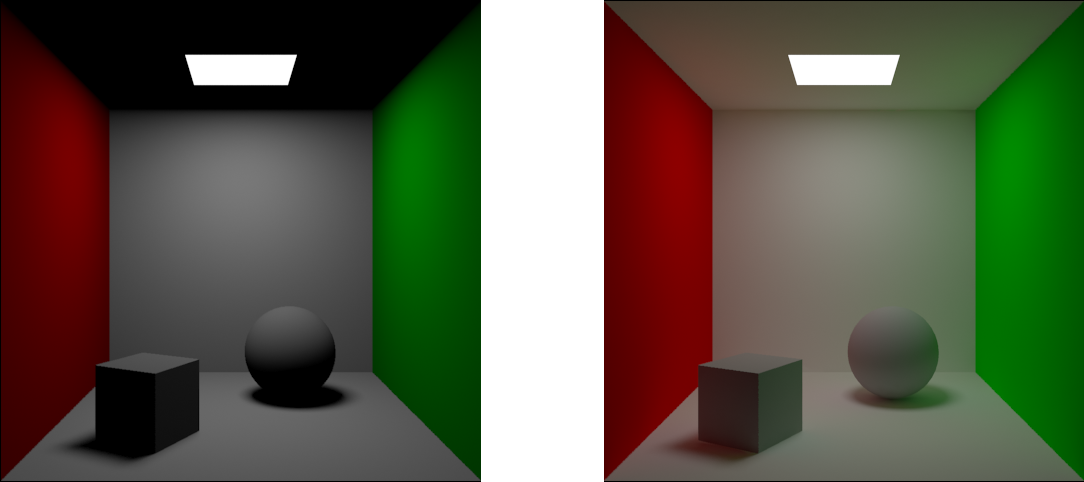
\includegraphics[width=3.0in]{img/GI-directAndIndirect.png}
	\caption[A global illumination example]{An example of global illumination. Left: direct illumination only. Right: direct plus indirect illumination. Scene: \textit{Cornell Box}. Notice the color bleeding effects with indirect illumination.}
	\label{fig:GI:directVSindir}
\end{figure}

\section{The Problem}
\label{sec:GI:problem}
The input of any renderer is a description of a virtual scene, with geometry information, light emitting information, surface material information, and possibly participating media information.
The output is, of course, imagery.
For the output to be realistic, the way each pixel is computed should reflect the true physics processes of light transport in the scene.

In the context of realistic image synthesis, many essentially identical concepts are often presented using different terminologies.
Light is a typical example, with names such as \textit{photon}, \textit{particle} or simply \textit{energy}.
For now we will simply call a single unit of light that we are interested in \textit{light}.
In this section, we will follow the path of \textit{light} from light sources all the way to the camera/eye/sensor.

The light source \textit{light} emitted from could be modeled in numerous ways.
It could be a point source, emitting light in all directions.
It could be a directional light source such that all peers are going in the same direction prior to initial bounce.
Most often light sources have an area, and emit light towards certain direction with a statistical distribution.
The way light sources are modeled affects the amount of energy each \textit{light} carries, thus the final distribution of energy in the scene.

After \textit{light} is emitted from a light source, it carries certain amount of energy.
The scene contains geometries and possibly participating media.
It is possible that \textit{light} will hit nothing and vanish.
In this case, it is a waste the resources allocated to compute \textit{light}.
More probably is that \textit{light} will hit a surface or reach a certain point in the participating media.
In this case, \textit{light} interacts with the surface or media.

The surface or media usually has a scattering model, or \textit{albedo}, which gives the distribution of outgoing direction given the incident direction of \textit{light}, as well as the fraction of the original energy that \textit{light} can get away with.
Take a red diffuse reflective surface for example.
The outgoing direction distribution is uniform in the upper hemisphere.
The fraction is determined by the \textit{albedo} of the surface.
After this scattering, \textit{light} will leave the surface carrying a bit of red in a random direction.

If by any chance, \textit{light} reaches the camera/eye/sensor only after first bounce, \textit{light} is contributing to direct illumination.
If not, it will continue traversing the scene.
After certain amount of bounces, \textit{light} may carry multiple information from previously visited surfaces and reach the camera/eye/sensor.
In this case, \textit{light} is contributing to indirect illumination.
It is probable that \textit{light} will not make it to the camera/eye/sensor.
In that case, it would be a potential waste.

Above process is illustrated in \figurename \ref{fig:GI:MrLight}.

\begin{figure}
	\centering
	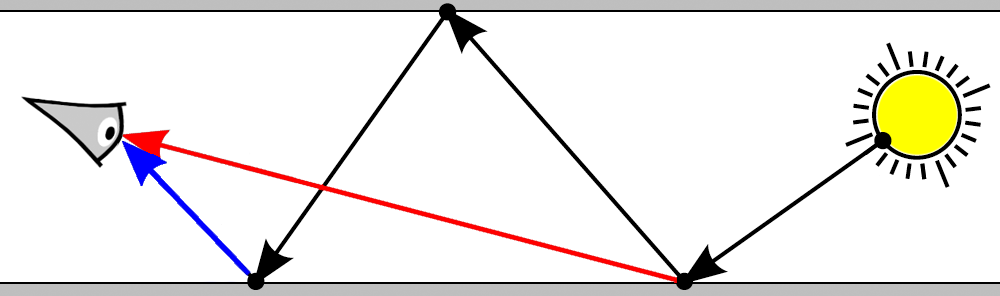
\includegraphics[width=3.0in]{img/GI-MrLight.png}
	\caption[Travel of \textit{light}]{The travel of \textit{light} from the light source to eye. The red arrow represents direct illumination, while the blue arrow represents indirect illumination.}
	\label{fig:GI:MrLight}
\end{figure}

\section{The Foundation}
\label{sec:GI:foundation}
Before we can formulate the above physical process, we need to lay some foundations.
In this section, we will briefly give the physical models of light, transport assumption and scattering models.

\subsection{Light Models}
\label{sec:GI:foundation:light}
Light, in its essence, is electromagnetic radiation \cite{PBRT3e}.
For human beings, the fraction that is perceived as visible light ranges approximately from \SI{380}{\nano \meter} to \SI{780}{\nano \meter} in wavelength.
\figurename \ref{fig:GI:SPD} gives an illustration of above description.

\begin{figure}[b]
	\centering
	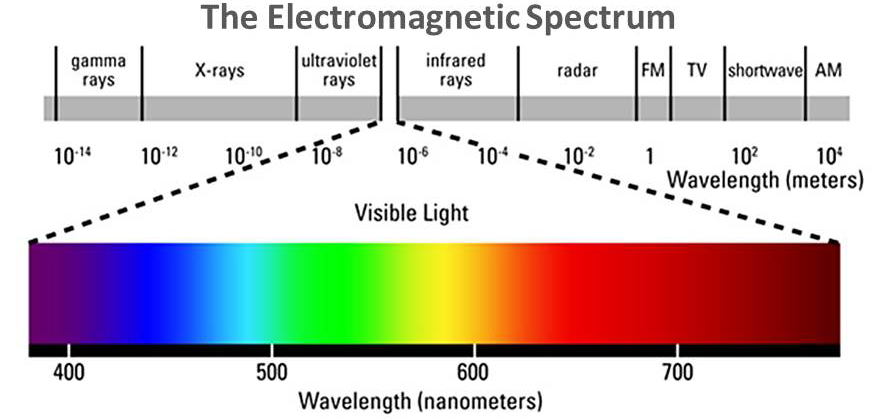
\includegraphics[width=4.0in]{img/GI-SPD.png}
	\caption[Visible Light Spectrum]{An illustration of visible light wavelength range in the electromagnetic radiation spectrum. (Image courtesy of \textit{Wikipedia})}
	\label{fig:GI:SPD}
\end{figure}

Visible lights are perceived as colors, which have unique \textit{spectral power distribution}s (SPDs).
Each SPD represents a histogram information over the whole visible frequency/wavelength range.
There are many successful color models with different application purposes.
Among those are \textit{CIE XYZ} color space, \textit{RGB} color model and \textit{CMYK} color model.

In real world, light have finite speed, even in vacuum.
With no participating media, light can travel \SI{299792458}{\meter \per \second}, or $1$ \textit{Planck unit}.
However, given the scope of scenes and application purposes, light in computer graphics are usually modeled to have infinite speed.
Furthermore, in real world, magnetic waves have effects such as diffraction and polarization when viewed at scales comparable to its wavelength.
This is far from feasible given modern computing hardware.
Geometric optics is the \textit{de facto} model of light used in computer graphics, for its simplicity.
In this model, light travels in straight lines with no energy loss, until a scattering event happens when light hits a surface or reach certain point in the participating media.

\subsection{Transport Simulation}
\label{sec:GI:foundation:transport}
\subsubsection*{Flux}
Flux, or radiant power, is a term used to measure how much energy is passing through a spatial region per unit time.
It is denoted as $\Phi$, with units in $watts$ (W, joules per second).

\subsubsection*{Irradiance and Radiance Exitance}
Irradiance (E) is the incident flux arriving at a surface, per unit area.
Radiance exitance (M) is the exitant radiant power leaving a surface, per unit area.
Both units are in $watts/m^2$.
\begin{equation}
	\label{eq:irradiance}
	E = \dfrac{d\Phi}{dA},\space M = \dfrac{d\Phi}{dA}.
\end{equation}

\subsubsection*{Solid Angle}
Solid angle is the 3D extension of \textit{planar angle}.
It is denoted as $\Omega$, with units in \textit{steradians} (sr).
While planar angle is the projected arc length onto a unit circle, solid angle is the projected area onto a unit sphere.
As shown in \figurename \ref{fig:GI:solidAngle}.
For example, the solid angle of a full sphere is $4\pi$ \textit{sr}.

In spherical coordinates, the differential solid angle is defined as

\begin{equation}
	\label{eq:solidAngle}
	d\Omega = \sin \theta d\theta d \varphi,
\end{equation}
where $\theta$ is the colatitude and $\varphi$ is the longitude.
Thus the solid angle can be calculated using the integral

\begin{equation}
	\Omega = \iint\limits_S \sin \theta d \theta d \varphi .
\end{equation}

\begin{figure}
	\centering
	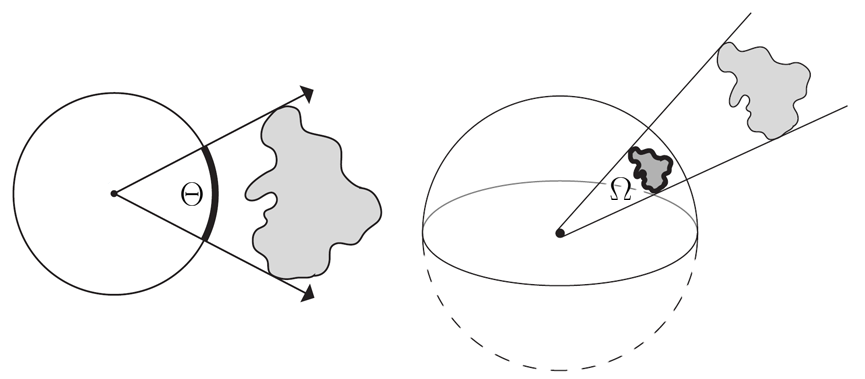
\includegraphics[width=3.0in]{img/GI-solidAngle.png}
	\caption[Solid angle]{Planar angle and its 3D analogue, solid angle. (Images courtesy of \citeauthor{PBRT3e})}
	\label{fig:GI:solidAngle}
\end{figure}

Notice that there is a mis-conception about how \eqref{eq:solidAngle} is derived.
It is usually considered to be an approximation of the area using a rectangle with differential edges.
However, in \textit{Riemannian Geometry}, there is solid derivation for \eqref{eq:solidAngle}.
The steps are beyond the scope of this survey, please refer to \cite{solidAngleDerivation} for more details.

\subsubsection*{Radiance}
Radiance (L) is the radiant power per unit projected area per unit solid angle.
The unit of radiance is in \textit{watts} / ($steradian \times m^2$ ).
Radiance can be incident or exitant power.

\begin{figure}
	\centering
	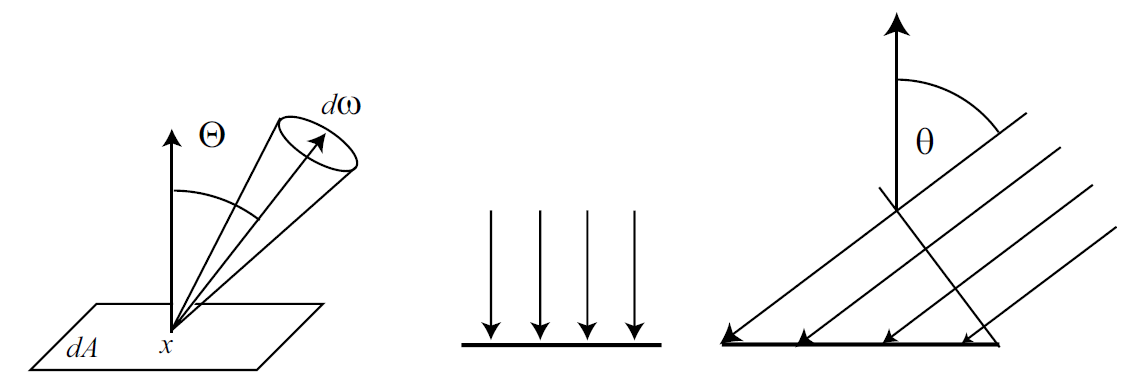
\includegraphics[width=4.0in]{img/GI-radiance.png}
	\caption[Definition of radiance]{The definition of radiance. (Images courtesy of \citeauthor{AdvancedGI})}
	\label{fig:GI:radiance}
\end{figure}

Radiance is a function of position and direction, see \figurename \ref{fig:GI:radiance}.
The definition of radiance is given by

\begin{equation}
	\label{eq:radiance}
	L(x, \Theta) = \frac{d^2 \Phi}{d \omega d A^\perp} = \frac{d^2 \Phi}{d \omega d A \cos \theta}.
\end{equation}

\subsection{Surface Scattering}
\label{sec:GI:foundation:scattering}
When light emitted from light sources hit a surface, or reach a certain point in the participating media, a scattering event happens.
Different materials have different scattering properties.
For example a perfect specular surface like the mirror only reflects light towards a direction that is uniquely determined by incident direction and surface normal.
A perfect diffuse surface reflects light towards all directions uniformly distributed in the upper hemisphere.
Glossy surfaces behaves somewhere in between.
\figurename \ref{fig:GI:BRDFs} illustrates how above three types of surfaces work.

\begin{figure}[b]
	\centering
	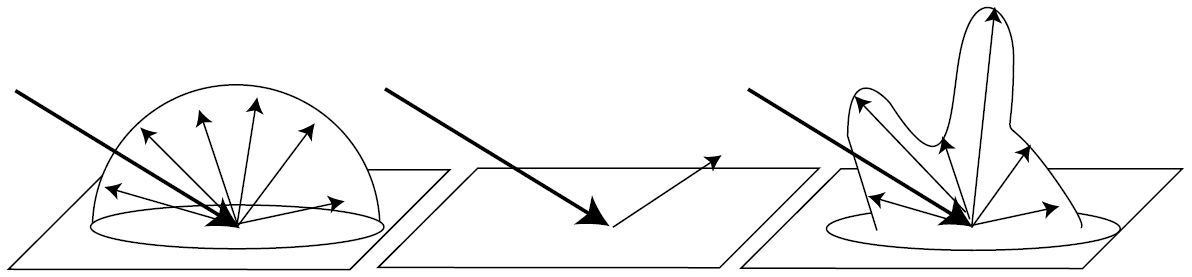
\includegraphics[width=4.0in]{img/GI-BRDFs.png}
	\caption[Surface Scattering]{Three different scattering models. Left: perfect diffuse reflection. Middle: perfect specular reflection. Right: glossy reflection. (Images courtesy of \citeauthor{AdvancedGI})}
	\label{fig:GI:BRDFs}
\end{figure}

\subsubsection*{BRDFs}
\textit{Bi-Directional Reflectance Distribution Functions} (BRDFs), are functions that model the fraction of incident flux that is reflected towards a specific direction.
This function usually takes as input incident direction, surface point, and outgoing direction.
The function is usually defined in the form of
\begin{equation*}
	f_{r}(\Psi, x, \Theta)
\end{equation*}
where $\Psi$ is the incident direction, $x$ is the scattering point, $\Theta$ is the outgoing direction.
This is often referred to as the hemispherical formulation.
BRDF can also be written in the form of
\begin{equation*}
	f_{r}(x_{i-i} \leftarrow x_{i} \leftarrow x_{i+1})
\end{equation*}
where $x_{i}$ is the scattering point, while $x_{i+1}$ and $x_{i-1}$ are previous point and next point along current path.
This is referred to as the area formulation or three point formulation.
Two formulations are essentially identical, but the latter proves more convenient for path space based techniques.

If we extend the model of BRDF to refractive surfaces, the function remains pretty much unchanged.
The only difference is that the outgoing direction now lies in the lower hemisphere.
This function is called \textit{Bi-Directional Transmittance Distribution Function}, or BTDF.
The generalization of BRDF and BTDF is BSDF, \textit{Bi-Directional Scattering Distribution Function}.
Notice that current model assumes the incident light and the outgoing light have a common point, the scattering point.
That is, the ending point of the incident light is the starting point of the outgoing light.
If we extend this further, and make the outgoing light initiating from a different point, we get the \textit{subsurface scattering effect}.

There are many BSDF models, and details of those are not the focus of this survey.
Please refer to \cite{AdvancedGI} and \cite{PBRT3e} for more information.

\subsubsection*{Physically Based Models}
One property to notice about BSDF models is that for a model to be physically based, it has to be energy conservative.
That is, the energy of all scattered outgoing light combined has to be no larger than the incident energy.
Expressed using the hemispherical formulation
\begin{equation}
	\int_{\Omega}f_{s}(\Psi, x, \omega) d\omega \leq 1
\end{equation}

Apart from energy conservation, a physically based model has to be reciprocal, i.e.\ $f_{s}(\Psi, x, \Theta) = f_{s}(\Theta, x, \Psi)$, thus the name \textit{bidirectional}.

\section{The Formulation}
\label{sec:GI:formulation}
Before we go into the details, we first briefly recap the history along the path.

The most classical style ray tracer is called \textit{Whitted-style}, which is named after \citeauthor{whitted1979improved} for he introduced the concept of using recursive ray tracing to solve reflection and refractions in \citeyear{whitted1979improved} \cite{whitted1979improved}.
However, Whitted-style ray tracers has its limitations, for it can only handle lighting in simple scenes with limited effects.

\citeauthor{cook1984distributed} introduced distributed ray tracing in \citeyear{cook1984distributed} \cite{cook1984distributed}, which can handle glossy reflections, area light sources, depth of field and motion blur with no additional work than regular Whitted-style.
This is achieved by randomly distributing samples in the BRDF, on the area light, on the camera lens and in time, respectively.

In \citeyear{kajiya1986rendering}, \citeauthor{kajiya1986rendering} formulated the global illumination problem as the rendering equation \cite{kajiya1986rendering}.
The equation, which is an integral in the form of a Fredholm equation of the second kind, has no deterministic solutions but the Monte Carlo numerical methods (see section \ref{sec:GI:formulation:MC}).
Interestingly enough, Monte Carlo methods was first applied in global illumination by the researchers in the Radiosity family.
Since Monte Carlo method is a stochastic process, the method \citeauthor{kajiya1986rendering} introduced is also called \textit{stochastic ray tracing}.
However, people favor the other name for this method, \textit{path tracing}, although it only appeared once in the original paper.

\citeauthor{ward1988IC} introduced the concept of irradiance caching in \citeyear{ward1988IC} \cite{ward1988IC}.
\citeauthor{krivanek2005radiance} build the concept of radiance caching \cite{krivanek2005radiance} on top of the work of \citeauthor{ward1988IC} in \citeyear{krivanek2005radiance}.
Irradiance caching and radiance caching are two methods that will be discussed in detail in chapter \ref{chap:ir-radiance}.

After this the border between gathering based and shooting based methods became unclear.
Many hybrid methods were introduced, such as \textit{bidirectional path tracing} (BDPT) \cite{lafortune1993bi, veach1995BDPT}, independently developed by \citeauthor{lafortune1993bi}, and \citeauthor{veach1995BDPT} and \textit{photon mapping} (PM) \cite{jensen1996global} by \citeauthor{jensen1996global}.
Photon mapping will be talked about in chapter \ref{chap:photon_mapping}.
In \citeyear{keller1997VPL}, \citeauthor{keller1997VPL} introduced \textit{instant radiosity} by using \textit{virtual point lights} (VPLs) to represent direct and indirect illumination.

The path towards efficient and robust solutions for global illumination problem has not yet come to an end.
The best from different sides can be eventually brought together, as we saw the recent advancement of combining photon mapping with bidirectional path tracing in \textit{vertex connection and merging} (VCM) \cite{georgiev2012light} or \textit{unified path sampling} (UPS) \cite{hachisuka2012path}, independently developed by \citeauthor{georgiev2012light} and \citeauthor{hachisuka2012path}.

\subsection{The Rendering Equation}
\label{sec:GI:formulation:equation}
The rendering equation is also known as the \textit{light transport equation}, which is essentially a \textit{Boltzmann transport equation}.
The original rendering equation is expressed in three-point formulation.
We will first present the hemispherical formulation, since it is easier to understand.
The rendering equation in hemispherical form is

\begin{gather}
\label{eq:renderEquation:hemisphere}
\begin{aligned}
	L(x \rightarrow \Theta) &= L_{e}(x \rightarrow \Theta) + L_{s}(x \rightarrow \Theta) \\&= L_{e}(x \rightarrow \Theta) + \int\limits_{\Omega_{x}} f_{s}(\Theta, x, \omega) L(x \leftarrow \omega) \left | \cos(N_{x}, \omega)\right | d\omega
\end{aligned}
\end{gather}
where:
\begin{itemize}
	\item[-] $L(x \rightarrow \Theta)$ is the radiance from surface point $x$ towards direction $\Theta$
	\item[-] $L_{e}(x \rightarrow \Theta)$ is the emitted radiance from surface point $x$, if the surface is non-emissive, this term is simply \textbf{0}
	\item[-] $L_{s}(x \rightarrow \Theta)$ is the scattered radiance from surface point $x$, which is intuitively the combination of all scattered incoming radiance from $\Omega_{x}$, thus the expansion
	\item[-] $\Omega_{x}$ is the hemisphere or sphere where incoming radiance may come from
	\item[-] $f_{s}(\Theta, x, \omega)$ is the BSDF
	\item[-] $L(x \leftarrow \omega)$ is the incoming irradiance from direction $\omega$
	\item[-] $\cos(N_{x}, \omega)$ is the cosine term for computing radiance coming from direction $\omega$.
\end{itemize}

Notice that in this formulation, we need to trace rays to get the radiance to be scattered, i.e.\ $L(x \leftarrow \omega)$.
The hemispherical form is intuitive, yet it is less convenient for path space based methods, for which paths containing vertices need to be constructed from the camera to light sources, or \textit{vice versa}.
The path vertices correspond to points in the three-point formulation, or area formulation.
This brings us to the three-point, or area form of the rendering equation, which is

\begin{gather}
\label{eq:renderEquation:threePoint}
\begin{aligned}
	L(x \leftarrow x') &= L_{e}(x \leftarrow x') + L_{s}(x \leftarrow x') \\ &= L_{e}(x \leftarrow x') + \int\limits_{A} f_{s}(x \leftarrow x' \leftarrow x'') L(x' \leftarrow x'') G(x' \leftrightarrow x'') dA(x'') \\
	G(x' \leftrightarrow x'') &= V(x' \leftrightarrow x'') \frac{\left| \cos\theta \right| \left| \cos{\theta}'\right|}{{\left\| x'' - x' \right\|}^2}
\end{aligned}
\end{gather}
where:
\begin{itemize}
	\item[-] $G(x' \leftrightarrow x'')$ is the geometry term between surface point $x'$ and $x''$
	\item[-] $A$ is all the surfaces that $x''$ could locate
	\item[-] $V(x' \leftrightarrow x'')$ is the visibility between $x'$ and $x''$, which is $1$ if they are mutually visible and $0$ otherwise
	\item[-] $\cos\theta$ and $\cos{\theta}'$ are cosine terms of $\vec{x'x''}$ with $N_{x'}$ and $\vec{x''x'}$ with $N_{x''}$
	\item[-] $\cos{\theta}'$ together with $\frac{dA(x'')}{{\left\| x'' - x' \right\|}^2}$ forms the differential solid angle
\end{itemize}

This is essentially identical to the hemispherical form, with only a few minor differences.
The first difference is that the integral transform from a integral over the (hemi)sphere to a integral over all surface points.
This is a different perspective to the same question.
The problem that comes along is that not all points are visible from current surface point, $x'$.
Thus the geometry term is introduce to handle both the solid angle issue and the visibility issue.

It is sometimes useful to explicitly write the equation in a form such that direct illumination and indirect illumination are separated.
In the three-point form, it is
\begin{gather}
\label{eq:renderEquation:dirIndir}
\begin{aligned}
	L(x_0 \leftarrow x') &= L_{e}(x_0 \leftarrow x') + L_{s}(x_0 \leftarrow x') \\ & = L_{e}(x_0 \leftarrow x') + L_{direct} + L_{indirect} \\
	L_{direct} &= \int\limits_{A_{e}} f_{s}(x_0 \leftarrow x' \leftarrow x'') L_{e}(x' \leftarrow x'') G(x' \leftrightarrow x'') dA(x'') \\
	L_{indirect} &= \int\limits_{A_{e^c}} f_{s}(x_0 \leftarrow x' \leftarrow x'') L_{s}(x' \leftarrow x'') G(x' \leftrightarrow x'') dA(x'')
\end{aligned}
\end{gather}
where $A_{e}$ is the set of all light source surfaces and $A_{e^c}$ is the set of all non emissive surfaces.

\subsection{Monte Carlo Methods}
\label{sec:GI:formulation:MC}
As mentioned earlier, the rendering equation, whether in hemispherical form or in three-point form, is a Fredholm equation of the second kind.
This means the term we are trying to solve also appears on the right side of the equation, hence a recursive nature.
For non-toy scenes, it is basically impossible to solve analytically.
The only practical solution is to use numerical methods.

\subsubsection*{Randomized Algorithms}
There are two families of randomized algorithms, viz.\ \textit{Las Vegas methods} and \textit{Monte Carlo methods} \cite{motwani1995randomized}.

If an algorithm can always gives correct result every time it is run, the only variation from one run to another is the running time, such an algorithm is called a \textit{Las Vegas method}.
A typical example is the \textit{Quicksort} algorithm.

If an algorithm can sometime output incorrect results, but the the probability of incorrect results can be bounded, such an algorithm is called a \textit{Monte Carlo method}.
This means that given enough runs with independent random inputs each time, the probability of producing incorrect results can be made arbitrarily small, i.e.\ the average results are statistically close to correct results.
The \textit{Min-cut} algorithm is a typical Monte Carlo method.

\subsubsection*{Monte Carlo integration}
For integration problems in real world applications, it usually turns out to be infeasible to compute analytically.
Monte Carlo integration is a technique based on the spirit of Monte Carlo methods to solve such problems.
The spirit is to use the expected value of some random samples to approximate the true integral.
To get the necessary Probability Theory background, please refer to the chapter on same topic in \cite{PBRT3e}, or \cite{MChandbook}.

Suppose we want to solve the integral for function $f(x)$ over domain $x\in \left [ a, b \right ]$
\begin{equation*}
	I = \int_{a}^{b} f(x) dx = \int_{a}^{b} \frac{f(x)}{p(x)} p(x) dx
\end{equation*}
where we can evaluate $f(x)$ but not the integral itself.
In Monte Carlo integration, an estimator is used to compute an estimation.
The estimator is denoted as $\widehat{I}$ and expressed as
\begin{equation*}
	\widehat{I} = \frac{1}{N} \sum_{i = 1}^{N}\frac{f(x_i)}{p(x_i)} 
\end{equation*}
where $p(x)$ is some \textit{probability density function} (PDF) from which $N$ random samples $x_i$ are sampled.

The strength of Monte Carlo integration is that it can handle complex integrals regardless of dimension or the presence of discontinuities.
Traditional numerical methods usually fail to converge at acceptable rates or even fail to converge at all when facing integrals in high dimensions or with discontinuities.
However, the downside of Monte Carlo method itself is that its convergence rate is of $O(1/\sqrt{n})$.
This means we have to evaluate four times more samples if we want to cut the variance in half.

\subsubsection*{Random Samples}
The way random samples are generated is very important for Monte Carlo integration.
The techniques we are about to discuss in later sections require that we could sample random variables according to an arbitrary distribution.

There are two basic ways to sample random variables given a specific PDF.
The first is to uniformly sample the inversed \textit{cumulative density function} (CDF).
The other is to reject a sample when the evaluated result of the sample is not what we want.
Full details are beyond the scope of this survey, please refer to \cite{PBRT3e} for details about inversed sampling and rejection methods, and \cite{MChandbook} for more sampling methods.

\subsubsection*{Importance Sampling}
Given the integral $\int f(x) dx$ as in \figurename \ref{fig:GI:importanceSampling}, if we were to sample according to the PDF in the left image, we might end up putting too many samples where values of $f(x)$ are low.
If we were to use the PDF in the middle image, we will get better results, but still lower than correct result.
Ideally, we would want to sample according to a PDF like the one in the right image.
Intuitively, the optimal PDF is
\begin{equation*}
	p(x) = \frac{\left| f(x) \right|}{\int f(x_i)dx_i},
\end{equation*}
but this is almost impossible since the denominator is the integral we are trying to solve.
\begin{figure}
	\centering
	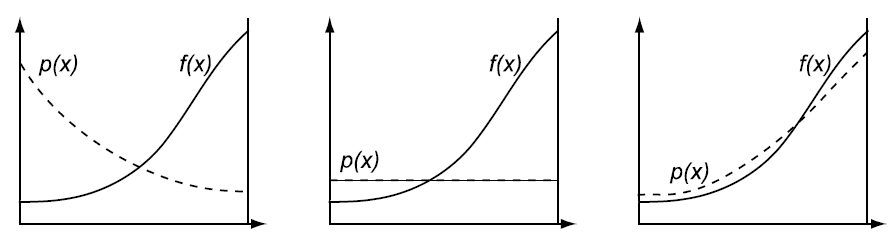
\includegraphics[width=4.0in]{img/GI-importanceSampling.png}
	\caption[Importance Sampling]{Three different sampling PDFs and the integral. (Images courtesy of \citeauthor{AdvancedGI})}
	\label{fig:GI:importanceSampling}
\end{figure}
This process is called \textit{importance sampling}, which is a major \textit{variance reduction} technique.
The core idea is to put more samples where the contribution is higher.
Many other variance reduction techniques also share the same spirit.

\subsubsection*{Markov Chain Monte Carlo}
A \textit{Markov Chain} is a sequence random events $\{X_1, X_2, \dots \}$ where the conditional probability of event $X_{i+1}$ given $\{X_1, X_2, \dots, X_i\}$ only depends on $X_i$.
The space of $X_i$ is called \textit{state space}, in which each element or event is called a \textit{state}.

\textit{Markov Chain Monte Carlo} (MCMC), like the original Monte Carlo method, also has a origin in the making of nuclear weapons \cite{MCMChandbook}.
It was introduced to simulate thermodynamic equilibrium by the same group of people who introduced Monte Carlo shortly after the introduction of Monte Carlo.
The Markov Chain Monte Carlo method is also called the \textit{Metropolis} algorithm, named after the researcher who invented it, or the \textit{Metropolis-Hastings} algorithm, joint-named after the research who generalized the original algorithm.

The core idea of MCMC is to start randomly in the state space.
In each step of the following steps, a new state is proposed by mutating current state.
A transition probability $p_t$ is calculated, together with the evaluation of the proposed state.
Then a random number $\xi$ is used to reject or accept the proposed state by comparing $\xi$ and $p_t$.
If the proposed state is rejected, current state along with its evaluation is recorded (again).
Otherwise the proposed state along with its evaluation is recorded.
The algorithm keeps running in this way until reaching equilibrium.

The power of MCMC is that it can guarantee \textit{ergodicity}.
Take the integral of $\int f(x) dx$ for example, MCMC could always give the correct evaluation without any \textit{a priori} knowledge of $f(x)$.
This property is referred to as \textit{perfect sampling}.
The original MCMC has the issue of \textit{startup bias}, which was solved by throwing away results from fist few pilot runs. 

The application of MCMC in global illumination is the \textit{Metropolis Light Transport} (MLT).
It was first introduced by \citeauthor{veach1997MLT} in \citeyear{veach1997MLT} \cite{veach1997MLT}.
The original MLT was implemented on top of BDPT, where the state space corresponds to the path space.
Please refer to the PhD thesis of \citeauthor{veach1997robust} for details \cite{veach1997robust}.
MLT has a number of variants, including \textit{primary sample space MLT} (PSSMLT), in which the state space corresponds to the space of random numbers that are used to generate path samples.
MLT is very good at handling difficult lighting situation, as it can explore important regions by its nature.
This can be seen in \figurename \ref{fig:GI:MLT}.

\begin{figure}
	\centering
	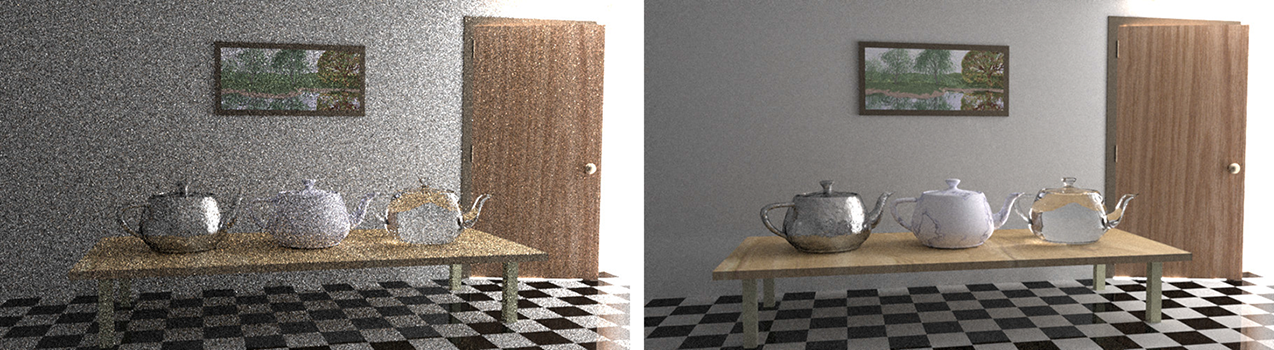
\includegraphics[width=4.0in]{img/GI-MLT.png}
	\caption[Metropolis Light Transport]{A difficult lighting scene \cite{veach1997robust}. The scene is lighted by a light source behind the door. All lights come through the gap. The left image is the result of regular BDPT, while the right image is the result of MLT with same rendering time. (Images courtesy of \citeauthor{veach1997robust})}
	\label{fig:GI:MLT}
\end{figure}

\section{The Trend}
\label{sec:GI:trend}
In \citeyear{veach1995MIS}, \citeauthor{veach1995MIS} introduced \textit{Multiple Importance Sampling} (MIS) into global illumination.
It was originally used to combine the contribution of different sampling strategies in importance sampling.
The Monte Carlo estimator with MIS is expressed as
\begin{gather}
\begin{aligned}
\widehat{I} &= \frac{1}{N} \sum_{i = 1}^{N} w(x_i) \frac{f(x_i)}{p(x_i)} \\
&= \frac{1}{N_f} \sum_{i = 1}^{N_f}w_f(x_i)\frac{f(x_i)}{p_f(x_i)} + \frac{1}{N_g} \sum_{j = 1}^{N_g} w_g(x_j)\frac{f(x_j)}{p_g(x_j)} \\
w_s(x_i) &= \frac{ (n_s p_s (x))^\beta}{(\sum_i n_i p_i (x))^\beta}
\end{aligned}
\label{eq:GI:MIS}
\end{gather}
where $p_f$ and $p_g$ are two sampling PDFs, $w_s(x)$ is a weighting function for strategy $p_s$, and $\beta$ is the exponent for the \textit{power heuristic}, which, according to \citeauthor{veach1995MIS}, gives good result when $\beta = 2$.
An example of MIS is shown in \figurename \ref{fig:GI:MIS}.

\begin{figure}[b]
	\centering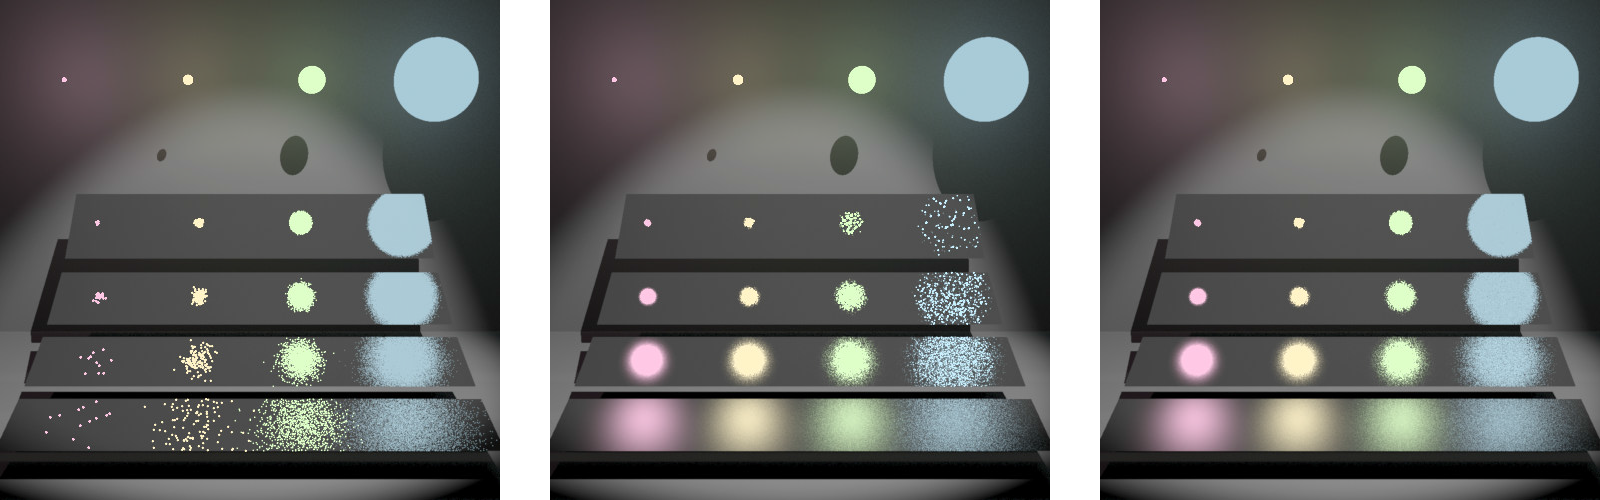
\includegraphics[width=4.0in]{img/GI-MIS.png}
	\caption[Multiple Importance Sampling]{An example of MIS \cite{veach1995MIS}. The left image is sampling the BSDF. The middle image is sampling lights. The right image is the combination of the two using MIS ($\beta = 2$). Surface properties vary from highly specular (1st board) to highly glossy (4th board). (Images courtesy of \citeauthor{veach1997robust})}
	\label{fig:GI:MIS}
\end{figure}

MIS is a bridging tool that brings together different powerful techniques.
The only problem is to solve the weighting function as different techniques typically do not belong to the same system, and it only makes sense to compute weights using probabilities when they lie in the same system.

Recent work of \citeauthor{georgiev2012light} and \citeauthor{hachisuka2012path} brings photo mapping and BDPT together using MIS \cite{georgiev2012light, hachisuka2012path}.
The work of \citeauthor{vsik2016robust} explores the combination of MLT and BDPT with VCM/UPS \cite{vsik2016robust}.
MIS is playing important roles in these new trends.

%%%%%%%%%%%%%%%%%%%%%%%%%%%%%%%%%%%%%%%%%%%%%%%%%%%%%%%%%%%%%%%%%%%%%%%%%%%%%%%%%%%%%%%%%%%%%%%%%%%%%%%%%%%%%%%%%%%%%%%%%%%%%%%%%%%%%%%%%%%%%%%%%%%%%%%%%%%%

\chapter{Irradiance and Radiance Caching}
\label{chap:ir-radiance}
\lettrine{I}{ndirect} illumination, as mentioned in the previous chapter, adds to the crucial part of realism for rendered images with global illumination.
From the knowledge of the previous chapter, we know that indirect illumination usually takes up the majority of the computation time, since we need to average many samples to get the result.
However, many research find that indirect illumination tend to vary smoothly over surfaces, as shown in \figurename \ref{fig:IC:coherence}.

\begin{figure}[!ht]
	\centering
	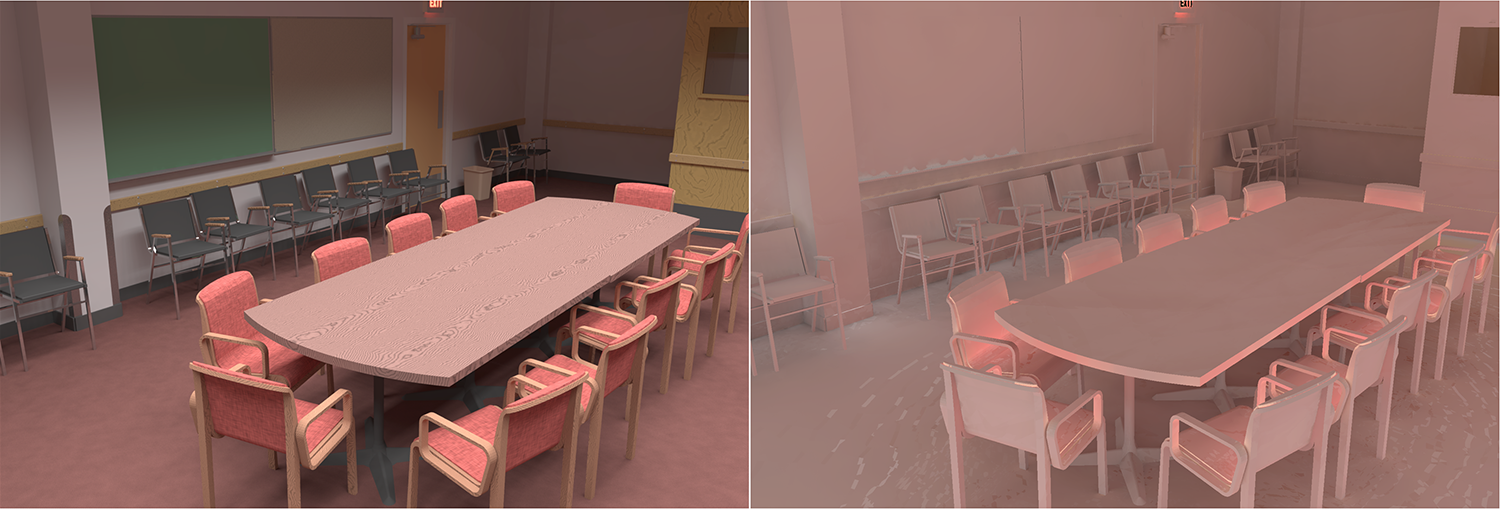
\includegraphics[width=5.0in]{img/IC-coherence.png}
	\caption[Indirect Illumination Coherence]{The rendering of the \textit{conference hall} scene. Left image shows global illumination. Right image shows indirect illumination only. Notice the slow changes of indirect illumination for points on the same surface. (Images courtesy of \citeauthor{ward1988IC})}
	\label{fig:IC:coherence}
\end{figure}

The core idea of irradiance caching is to exploit this smoothness and only evaluate irradiance using sampling at a sparsely distributed set of points on scene surfaces and store them for later use.
Irradiance at later points are evaluated by interpolating between caches of available records.
New cache records are created when no caches are available.
\citeauthor{ward1988IC} first introduced this idea in \citeyear{ward1988IC} \cite{ward1988IC}.

Since irradiance is the incident flux at surfaces, irradiance caching is limited to outgoing direction independent surfaces only, i.e., diffuse surfaces.
Radiance caching is introduced by \citeauthor{krivanek2005radiance} in \citeyear{krivanek2005radiance} \cite{krivanek2005radiance}.
Radiance caching is a generalization of irradiance caching by augmenting caches with complex directional incident distribution.
The result is that glossy surfaces can also work with caching scheme.

In this chapter, we first discuss the details of irradiance caching and then present the modification of radiance caching to irradiance caching.
In section \ref{sec:IC:icoverview}, we present the algorithm overview.
In section \ref{sec:IC:data}, we discuss what data to store, how to calculate them and the data structure to store them.
Section \ref{sec:IC:usingdata} is about the way caches are used during the rendering process.
Finally, we present the addition and modification of radiance caching to irradiance caching in section \ref{sec:IC:radiance}.

\section{Irradiance Caching Overview}
\label{sec:IC:icoverview}
The overall algorithm of irradiance caching is shown in \textcolor{blue}{Algorithm \ref{alg:IC:overview}}.
An illustration of one demonstration process is given in \figurename \ref{fig:IC:overview}.

\begin{algorithm}[t]
\caption[Irradiance Caching]{Pseudo code for Irradiance Caching.}
\addtocontents{loa}{\vskip 4pt}
\label{alg:IC:overview}
\begin{algorithmic}[1]
\Procedure{IrradianceCaching}{\textbf{p}}
	\State query \textbf{p} in the data structure
	\If{one or more records available for interpolation around point \textbf{p}}
		\State interpolate using values and gradients from available records
		\State \Return interpolated irradiance value
	\Else
		\State calculate irradiance value and irradiance gradients using hemispherical sampling
		\State store new value and gradients as a new record in the data structure
		\State \Return new irradiance value
	\EndIf
\EndProcedure
\end{algorithmic}
\end{algorithm}

\begin{figure}[b]
	\centering
	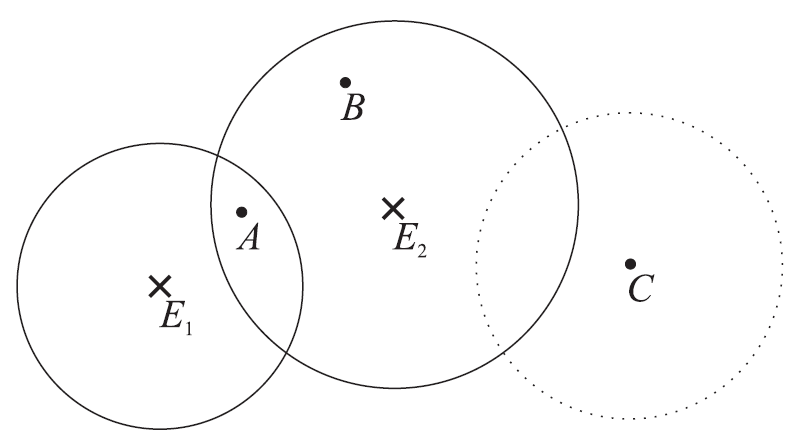
\includegraphics[width=3.0in]{img/IC-overview.png}
	\caption[Irradiance Caching]{The overall scheme of irradiance caching. Two existing records $E_1$ and $E_2$. For point $A$, irradiance value is the interpolation between $E_1$ and $E_2$. For point $B$, irradiance value is the interpolation of $E_2$. For point $C$, a new record has to be calculated and inserted into the data structure. (Image courtesy of \citeauthor{ward1988IC})}
	\label{fig:IC:overview}
\end{figure}

When no records are available, irradiance values and gradients are calculated at each point using Monte Carlo techniques, i.e.\ sampling.
Otherwise an interpolated result is returned.
\textit{Irradiance Gradients} \cite{ward1992irradiance} is a piece of geometric information at \textbf{p} that can be calculated along with the irradiance value without additional cost.
It is used in the interpolation phase.

In \textcolor{blue}{Algorithm \ref{alg:IC:overview}}, line $2$ and $8$ correspond to section \ref{sec:IC:data:structure}.
Line $3$ corresponds to section \ref{sec:IC:usingdata:determine}.
Line $4$ corresponds to section \ref{sec:IC:usingdata:interpolate}.
Line $7$ corresponds to section \ref{sec:IC:data:represent} and \ref{sec:IC:data:compute}.

\section{Cache Data and Data Structure}
\label{sec:IC:data}
During stochastic ray tracing, we only sample one secondary ray per bounce per iteration and average the results of many iterations to get the final result.
This progressive style calculation is prohibitive for calculating cached data, as the later use of caches is based on the assumption that they are accurate enough as a reference.
This means, for each cache record, we need to capture irradiance from all directions arriving at current point before we store it as a valid record
\begin{equation}
\label{eq:IC:irradiance}
E(\textbf{p}) = \int_{H^+} L_i(\textbf{p}, \omega) \cos\theta d\omega
\end{equation}
where $H^+$ is the upper hemisphere over \textbf{p}, $L_i(\textbf{p}, \omega))$ is the incoming radiance from direction $\omega$, and $\theta$ is the absolute angle formed by $-\omega$ and surface normal $N_{\textbf{p}}$.

\subsection{Data Representation}
\label{sec:IC:data:represent}
Since the surfaces irradiance caching are dealing with are diffuse surfaces, plus the fact that no \textit{a priori} knowledge is given about the scene, the only importance sampling technique we could use is \textit{cosine weighted hemispherical sampling}, as the irradiance are weighted by the cosine term.
The PDF for hemispherical sampling is
\begin{equation}
\label{eq:IC:PDF}
	p(\theta, \phi) = \frac{\cos(\theta)}{\pi}
\end{equation} 
where $\pi$ exists so that $\int_{0}^{\pi / 2}p(\theta, \phi)d\theta = 1$.

\textit{Stratification} is used to make the hemisphere better covered.
The hemispherical coordinate $\theta$ and $\phi$ are stratified into $M$ and $N$ strata respectively.
Within each stratum, one sample is generated.
The estimator for irradiance at point \textbf{p} is
\begin{equation*}
	\widehat{E}(\textbf{p}) = \frac{1}{MN} \sum_{j=0}^{M-1} \sum_{k=0}^{N-1} \frac{f(\theta_{j, k}, \phi_{j, k})}{p(\theta_{j, k}, \phi_{j, k})},
\end{equation*}
where $\theta_{j,k}$ and $\phi_{j,k}$ are each determined by two random numbers $\xi_{j, k}^{1}$ and $\xi_{j, k}^{2}$ using following equation
\begin{gather}
\label{eq:IC:hemisphericalCoord}
\begin{aligned}
	\theta_{j,k} &= \arccos \sqrt{1 - \frac{j + \xi_{j, k}^{1}}{M}}, \\
	\phi_{j,k} &= 2\pi\frac{k + \xi_{j, k}^{2}}{N}.
\end{aligned}
\end{gather}

With reference to Equation \ref{eq:IC:irradiance}, where $f(\theta, \phi) = L_i(\textbf{p}, \omega) \cos\theta$ and Equation \ref{eq:IC:PDF}, we get
\begin{equation}
\label{eq:IC:irradianceEstimator}
	\widehat{E}(\textbf{p}) = \frac{\pi}{MN} \sum_{j=0}^{M-1} \sum_{k=0}^{N-1} L_{j, k} (\textbf{p}, \theta_{j, k}, \phi_{j, k}).
\end{equation}

\subsubsection*{Irradiance Gradients}
During the rendering phase, irradiance values are interpolated.
To better weight available records, it is better to have few geometric information.
Intuitively, point position and surface normal information are necessary.
Irradiance gradients are introduced by \citeauthor{ward1992irradiance} to provide more information than merely position and normal \cite{ward1992irradiance}.
It provides the first-order approximation of irradiance changes, c.f.\ derivatives of functions.

Two gradients are defined to capture above information, viz.\ \textit{rotation gradient} and \textit{translation gradient}.
Usually different channels in color models have different gradients.

Rotation gradient gives the rotational axis vector about which the irradiance changes most quickly.
The magnitude of the gradient vector denotes the slope in that direction, i.e.\ how quick is the change.
Rotation gradient is calculated along with the calculation of irradiance value, since no additional information is required.
It is denoted as $\nabla_{r}E$ and is expressed as
\begin{equation}
\label{eq:IC:rotation}
	\nabla_r E \approx \frac{\pi}{MN} \sum_{k=0}^{N-1}\left({\textbf{v}}_k \sum_{j-0}^{M-1} - \tan \theta_j L_{j,k}\right)
\end{equation}
where ${\textbf{v}}_k$ is a vector in the tangent plane at \textbf{p} in direction $\phi_k + \frac{\pi}{2}$, $L_{j,k}$ is the sampled incoming radiance for stratum $(j,k )$, same as the radiance term in Equation \ref{eq:IC:irradiance}.
%where ${\textbf{v}}_k$ is a vector in the tangent plane at \textbf{p} in direction $(\pi/2, \phi_k + \frac{\pi}{2})$, $L_{j,k}$ is the sampled incoming radiance for stratum $(j,k )$, same as the radiance term in Equation \ref{eq:IC:irradiance}.

Translation gradient is an analogue of rotation gradient, only the domain is smaller, as we only care about the change along the surface.
For this reason, translation gradient only take into account the changes in the tangent plane. 
Translation gradient is denoted as $\nabla_{t}E$ and expressed in a much more complex way as
\begin{equation}
\begin{split}
	\nabla_{t}E \approx \sum_{k=0}^{N-1} \Bigg[ &\textbf{u}_k \frac{2\pi}{N} \sum_{j=1}^{M-1} \frac{\cos^2\theta_{j_-}\sin\theta_{j_-}}{\textup{min}(r_{j,k}, r_{j-1,k})} \left( L_{j,k}-L_{j-1,k} \right ) + \\
	&\textbf{v}_{k_-} \sum_{j=0}^{M-1} \frac{\cos\theta_j \left( \cos\theta_{j_-} - \cos\theta_{j_+} \right )}{\sin\theta_{j,k} \textup{min}(r_{j,k}, r_{j,k-1})} \left( L_{j,k}-L_{j,k-1} \right ) \Bigg]
\end{split}
\end{equation}
where:
\begin{itemize}
	\item[-] $r_{j,k}$ is the distance the sample ray in stratum $(j,k)$ travels before hitting something
	\item[-] $\theta_{j_-} = \arccos\sqrt{1-\frac{j}{M}}$
	\item[-] $\theta_{j_+} = \arccos\sqrt{1-\frac{j+1}{M}}$
	\item[-] $\textbf{u}_k$ is a vector in the tangent plane at \textbf{p} in direction  $(\pi/2, \phi_k)$, $\phi_k = 2\pi\frac{k+0.5}{N}$
	\item[-] ${\textbf{v}}_{k_-}$ is a vector in the tangent plane at \textbf{p} in direction $(\pi/2, \phi_{k_-} + \pi/2)$, $\phi_{k_-} = 2\pi\frac{k}{N}$
\end{itemize}

Just like rotation gradient gives the rotational axis information w.r.t.\ irradiance changes, translation gradient gives the direction in the tangent plane along which the irradiance changes the fastest.
The magnitude of translation gradient represents how fast the change is.

Data to be stored includes irradiance value, rotation gradient, translation gradient and point position and normal.
The first term is a vector valued color, e.g.\ RGB color.
The gradients are three-dimensional vectors.

\subsection{Data Calculation}
\label{sec:IC:data:compute}
The way data calculated is a typical Monte Carlo process.
The only difference from regular rendering is that at each diffuse bounce, the incoming radiance from the full hemisphere is calculated using Equation \ref{eq:IC:irradianceEstimator} instead of only one sample per iteration.
In each of the $M\cdot N$ strata, a ray is shot towards a direction according to Equation \ref{eq:IC:hemisphericalCoord}, which can be easily mapped to world space from local space.
Given the equations in the previous section, all necessary data can be calculated in a straightforward way.
An example of stratified hemisphere with incoming radiance calculated is shown in \figurename \ref{fig:IC:hemisphere}.

There is a matter of style in caching schemes, two-pass or progressive.
The original irradiance caching algorithm as shown in \textcolor{blue}{Algorithm \ref{alg:IC:overview}} shows a progressive nature.
However, n{\"a}ive implementation would lead to artifacts.

Consider a surface point like point $B$ in \figurename \ref{fig:IC:overview}.
The only available cache record is $E_2$.
If no more records were to be created and added in the empty region around $E_2$, many vicinity points within the affective radius of $E_2$ would be only affected by $E_2$.
This is a major cause of artifacts.
Many methods have been proposed to handle this, such as the \textit{Best Candidate Pattern} \cite{PBRT3e}, which resembles a \textit{Poisson process}.

Ideally, we would like to render with many cache records already available and distributed in such a way that the surfaces in the scene are covered well enough.
This leads to the most popular way of doing irradiance caching, a two-pass style.
In the first pass, cache records are created and stored in the data structure.
Typically one cache record per pixel to better cover the image.
In the second pass, cache records are interpolated to generate final render.
One good feature of the two-pass style is that we can still add new records in the second pass.
This can be done by simply setting the search radius smaller, so that gaps will appear between existing cache records.

\begin{figure}
	\centering
	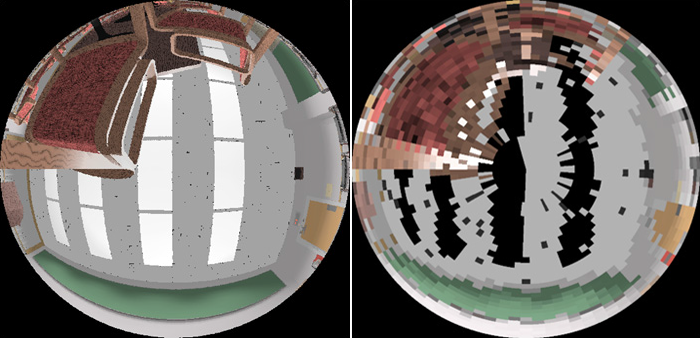
\includegraphics[width=4.0in]{img/IC-hemisphere.png}
	\caption[Irradiance Cache Data]{Left: a fish-eye view of a point on the floor in \figurename \ref{fig:IC:coherence}. Right: stratified view of indirect illumination from the same point. Notice the black areas in the right image. This is because all direct illumination are ignored and these strata corresponds to lights. Values from all strata are averaged to approximavicinityte the incoming radiance of the full hemisphere. (Images courtesy of \citeauthor{ward1988IC})}
	\label{fig:IC:hemisphere}
\end{figure}

\subsection{Data Structures}
\label{sec:IC:data:structure}
The whole point of using caching in the first place is that it should be faster than direct computation.
Therefore the data structure should be efficient at handling cache queries.
Apart from queries, one other important task for a spatial structure is to update the structure by inserting new records.
Even though record deletion is not used in this case, it turns out to be useful for other caching techniques, as we will see in later chapters.

Intuitively, it should be a spatial structure, since the query entry is point position and normal information.
One way is to directly store cache records at surfaces, i.e.\ via storing at vertices or texturing.
However, this makes query for nearest points from different objects hard and adds to the complexity of the scene geometry query structure.
Therefore, a better way is to maintain a separate spatial structure for irradiance caches.
As we will shortly see in Section \ref{sec:IC:usingdata:interpolate}, each usable cache record is assigned a weight value during interpolation.
This requires usable records to be within certain radius.
Each record also possesses a spatial extent as defined in gradients, i.e.\ a cache record has a radius.

Give the requirements above, the optimal structure is a k-dimensional tree (k-d tree) or an octree.
In the original paper, an octree is used to store records.
Each record is referenced by a node in the octree.
The node contains record position information and the size of the node is proportional to the radius of the record, which is determined by record gradients.
The pseudo code for query in the octree is given in \textcolor{blue}{Algorithm \ref{alg:IC:octreeSlow}}, where $w_i(\textbf{p})$ is a weighting function used to assign each usable record a weight.
Details will be shortly presented in Section \ref{sec:IC:usingdata:interpolate}.

\begin{algorithm}[!ht]
\caption[Slow Octree Query]{Pseudo Code for Cache Octree Query - Slow}
\addtocontents{loa}{\vskip 4pt}
\label{alg:IC:octreeSlow}
\begin{algorithmic}[1]
\Procedure{CacheOctreeSlowQuery}{\textbf{\textit{node}}, \textbf{p}}
	\ForAll{cache records $\textbf{r}_i$ in \textbf{\textit{node}}}
		\If{$w_i(\textbf{p})>0$ \textbf{and} $\textbf{p}_i$ not in front of \textbf{p}}
			\State report $\textbf{r}_i$
		\EndIf
	\EndFor
	\ForAll{children \textbf{\textit{child}} of \textbf{\textit{node}}}
		\If{\textbf{p} is no further away than half the cube size of \textbf{\textit{child}} from its boundary}
			\State \textsc{CacheOctreeSlowQuery}(\textbf{\textit{child}}, \textbf{p})
		\EndIf
	\EndFor
\EndProcedure
\end{algorithmic}
\end{algorithm}

\textsc{CacheOctreeSlowQuery} is named \textit{slow} because all children are recursively examined under relevant nodes.
An improvement could be made by referencing a record to all overlapping nodes within a valid distance.
The improved query algorithm is given in \textcolor{blue}{Algorithm \ref{alg:IC:octreeFast}}.
2D illustrations of octree structure are given in \figurename \ref{fig:IC:octree}.

\begin{algorithm}[!ht]
\caption[Fast Octree Query]{Pseudo Code for Cache Octree Query - Fast}
\addtocontents{loa}{\vskip 12pt}
\label{alg:IC:octreeFast}
\begin{algorithmic}[1]
	\Procedure{CacheOctreeFastQuery}{\textbf{\textit{node}}, \textbf{p}}
		\State \textbf{\textit{node}} $\gets$ \textbf{\textit{root}}
		\While{\textbf{\textit{node}}$\neq$NULL}
			\ForAll{cache records $\textbf{r}_i$ in \textbf{\textit{node}}}
				\If{$w_i(\textbf{p})>0$ \textbf{and} $\textbf{p}_i$ not in front of \textbf{p}}
					\State report $\textbf{r}_i$
				\EndIf
			\EndFor
			\State \textbf{\textit{node}} $\gets$ child node containing \textbf{p}
		\EndWhile
	\EndProcedure
\end{algorithmic}
\end{algorithm}

\begin{figure}[!ht]
	\centering
	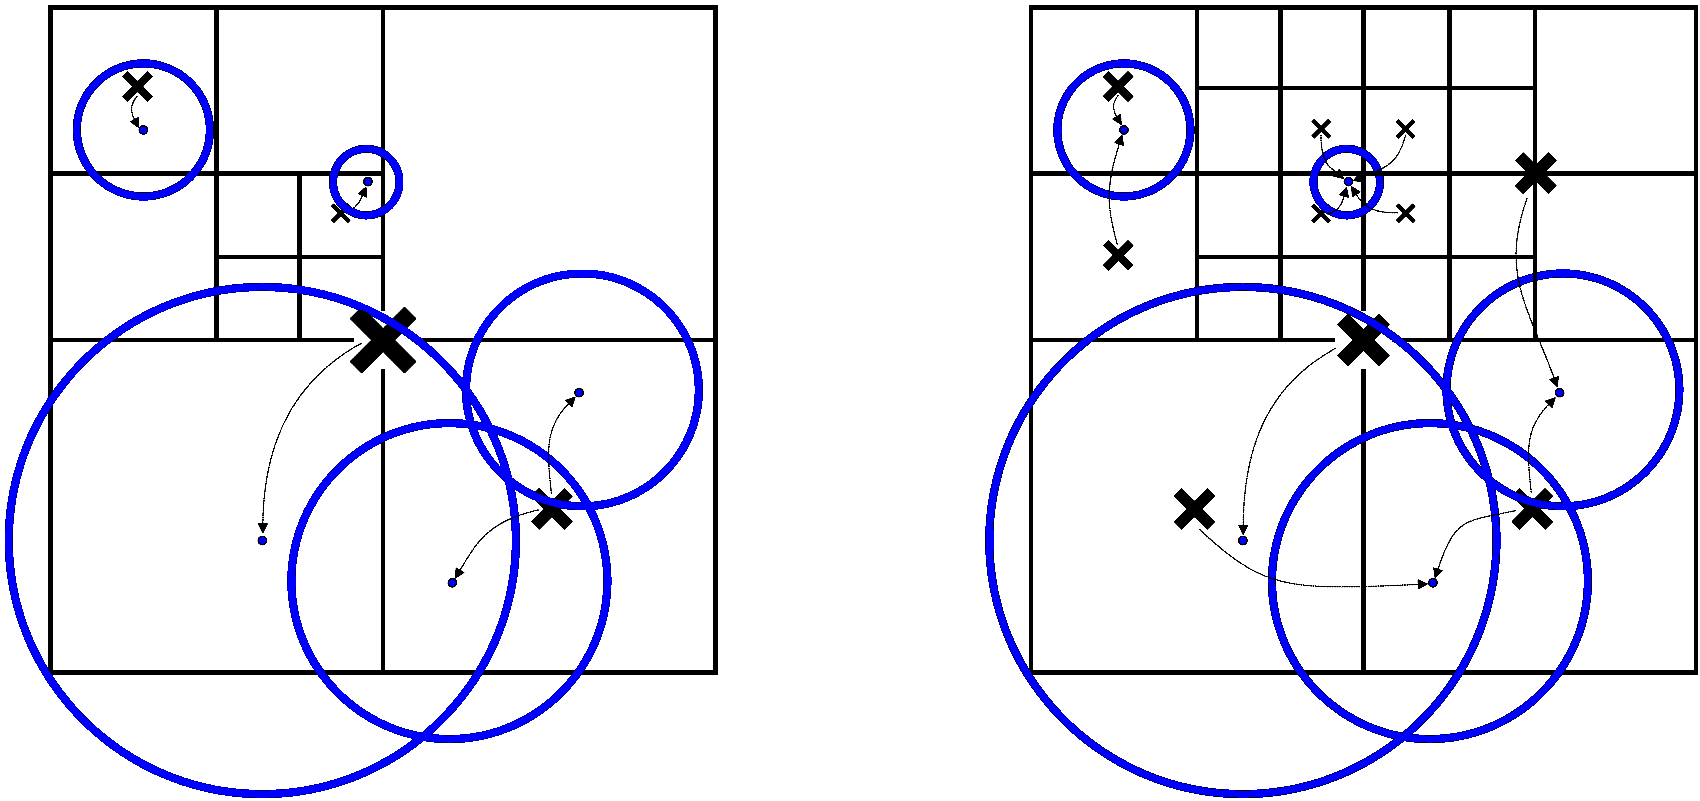
\includegraphics[width=3.0in]{img/IC-structure.png}
	\caption[Irradiance Cache Octree]{2D illustrations of record reference assignment for an octree. Left: single referenced octree. Right: multiple referenced octree. (Images courtesy of \citeauthor{ward1992irradiance})}
	\label{fig:IC:octree}
\end{figure}

\section{Rendering Using Cache Data}
\label{sec:IC:usingdata}
As shown in \textcolor{blue}{Algorithm \ref{alg:IC:overview}}, during rendering, usable records, if any, are queried and interpolated to get the final result.
Given the query structure, i.e.\ octree, we need to further define some terms before completion.

\subsection{Determine Usable Records}
\label{sec:IC:usingdata:determine}
As in line 3 of \textcolor{blue}{Algorithm \ref{alg:IC:octreeSlow}} or line 5 of \textcolor{blue}{Algorithm \ref{alg:IC:octreeFast}}, a weighting term need to be defined for a record to be considered \textit{usable}.
The weighting term $w_i(\mathbf{p})$ of record $\mathbf{r}_i$ for query point \textbf{p} is expressed as
\begin{equation}
\label{eq:IC:weight}
	w_i(\mathbf{p})=\frac{1}{\frac{\left \| \mathbf{p} - \mathbf{p}_i \right \|}{R_i} + \sqrt{1-\mathbf{n}\cdot \mathbf{n}_i}}-\frac{1}{\alpha}
\end{equation}
where:
\begin{itemize}
	\item[-] $\mathbf{p}$ and $\mathbf{p}_i$ are positions for point and record $\mathbf{r}_i$
	\item[-] $\mathbf{n}$ and $\mathbf{n}_i$ are normals for point and record $\mathbf{r}_i$
	\item[-] $R_i$ is a distance calculated along with irradiance value and gradients, which is the average distance to visible surfaces
	\item[-] $\alpha$ is a user specified value to tweak for error
\end{itemize}

All records with non-zero weight are considered usable records, only their contribution are scaled by different weights.

\subsection{Advanced Interpolation}
\label{sec:IC:usingdata:interpolate}
The final irradiance at point \textbf{p} is calculated as the weighted average of all usable records.
Rotation and translation gradients are exploited here to yield a better result.
The final irradiance value $E(\mathbf{p})$ is calculated as
\begin{gather}
\label{eq:IC:interpolation}
\begin{aligned}
	E(\mathbf{p}) &= \frac{\sum_i E_i(\mathbf{p})w_i(\mathbf{p})}{\sum_i w_i(\mathbf{p})}, \\
	E_i(\mathbf{p}) &= E_i + (\mathbf{n}_i \times \mathbf{n}) \cdot \nabla_r E_i + (\mathbf{p} - \mathbf{p}_i) \cdot \nabla_t E_i .
\end{aligned}
\end{gather}

\section{Radiance Caching}
\label{sec:IC:radiance}
As mentioned at the beginning of the chapter, irradiance caching mainly targets at indirect illumination for pure diffuse surfaces.
This is the major limitation.

Recall in Section \ref{sec:GI:foundation:scattering}, three types of surfaces exist.
For pure specular surfaces, no stochastic evaluation is needed, since they can be handled deterministically.
For glossy surfaces, BSDF models thereof are view-dependent.
To make irradiance caching scheme compatible with glossy surfaces, the incoming direction information need to be cached along with incoming radiance values.

This is the core idea of radiance caching, that is to cache the directional distribution of incoming radiance at a surface point.
The presence of this additional directional distribution information makes it possible to calculate radiance for glossy surfaces.

It is necessary to notice that both irradiance caching and radiance caching are biased techniques.
Since the cached values are directly used for final render, bias is inevitable.
There are many improvements toward both methods, including making the scheme adaptive and improving error controls.

%%%%%%%%%%%%%%%%%%%%%%%%%%%%%%%%%%%%%%%%%%%%%%%%%%%%%%%%%%%%%%%%%%%%%%%%%%%%%%%%%%%%%%%%%%%%%%%%%%%%%%%%%%%%%%%%%%%%%%%%%%%%%%%%%%%%%%%%%%%%%%%%%%%%%%%%%%%%

\chapter{Photon Mapping}
\label{chap:photon_mapping}
\begin{figure}[!ht]
	\begin{subfigure}{0.24\textwidth}
		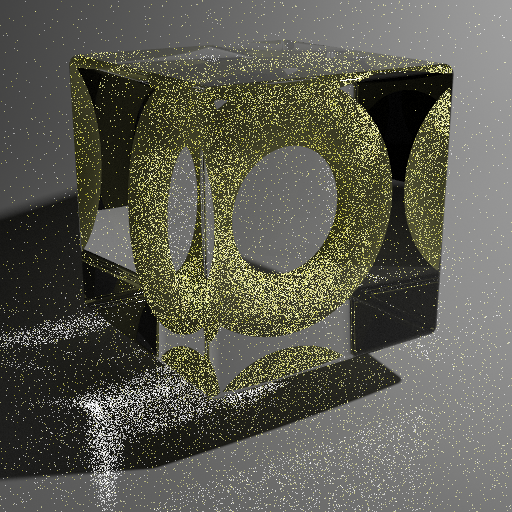
\includegraphics[height=1.4in]{img/PM-0-PT.png}
		\caption{PT}
	\end{subfigure}%
	~
	\begin{subfigure}{0.24\textwidth}
		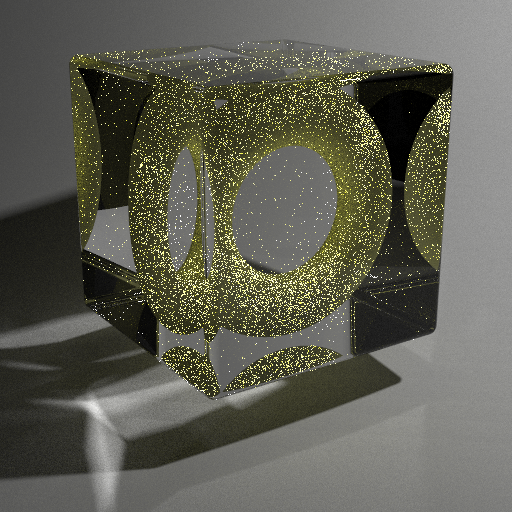
\includegraphics[height=1.4in]{img/PM-0-BDPT.png}
		\caption{BDPT}
	\end{subfigure}%
	~
	\begin{subfigure}{0.24\textwidth}
		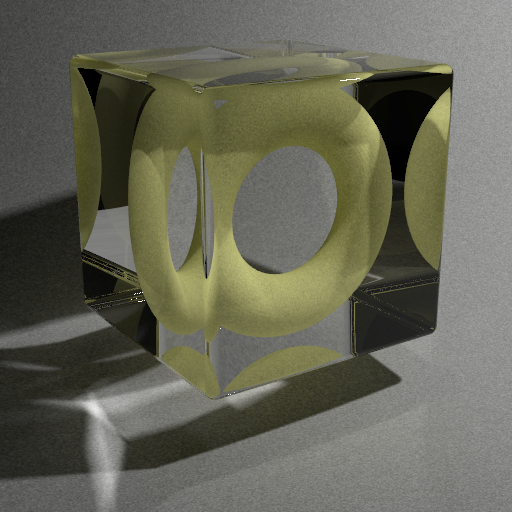
\includegraphics[height=1.4in]{img/PM-0-PM.png}
		\caption{Photon Mapping}
	\end{subfigure}%
	~
	\begin{subfigure}{0.24\textwidth}
		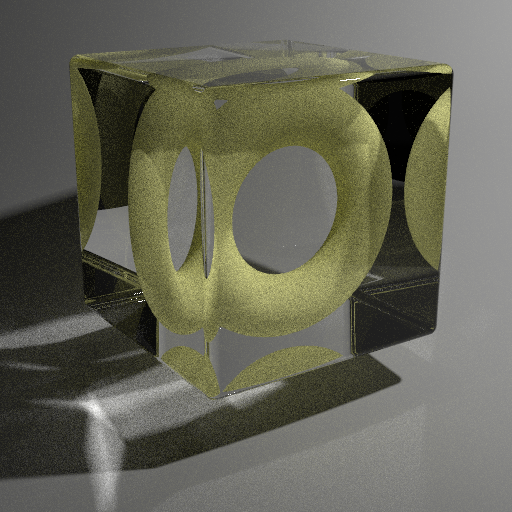
\includegraphics[height=1.4in]{img/PM-0-reference.png}
		\caption{Reference}
	\end{subfigure}
	\caption[Photon Mapping Comparison]{A comparison of different techniques. Scene: diffuse torus in a specular box. The reference image is generated using path tracing with $51,500$ samples per pixel. Other three images were rendered with same amount of time. Notice how path tracing fails to efficiently capture the caustics in image (a). BDPT did capture caustics efficiently, however, it fails to efficiently capture specular-diffuse-specular paths. (Images courtesy of \citeauthor{jensen1996global} and \citeauthor{hachisuka2008progressive})}
	\label{fig:PM:compare}
\end{figure}

\lettrine{T}{raditional} ray tracing and Monte Carlo ray tracing techniques are both gathering based techniques.
The irradiance and radiance caching fall in this category as well.
Shooting based techniques, like \text{light tracing} \cite{dutre1993lighttrace}, a.k.a.\ \textit{particle tracing}, faithfully represents the physical process that is really going on in real world: light travels from light sources to eyes.
However, pure light tracing algorithm is generally considered inefficient for the same reason we briefly mentioned in Chapter \ref{chap:GI}.
BDPT, as a typical hybrid method, inherit good features from both gathering methods and shooting methods.
However, for the notoriously difficult lighting situations, specular-diffuse-specular paths, BDPT performs poorly.
A comparison of photon mapping with other techniques is shown in \figurename \ref{fig:PM:compare}.

The core motivation for photon mapping is to distribute illumination in the scene and render with this pre-calculated data.
This pre-calculated illumination can be used in several ways, as we will discuss in detail in this chapter.
In section \ref{sec:PM:overview} we present the photon mapping algorithm overview.
We discuss about the data used in photon mapping, i.e.\ photons, and the data structure, i.e.\ photon map, in section \ref{sec:PM:data}.
Section \ref{sec:PM:render} is about how to use the photon map during rendering.

\section{Photon Mapping Overview}
\label{sec:PM:overview}
Irradiance caching, as discussed in the previous chapter, pre-calculates and stores illumination information from a gathering point of view, i.e.\ eye-driven.
Photon Mapping is working the other way around from a shooting point of view, i.e.\ light-driven.

\subsection{The Algorithm}
\label{sec:PM:overview:algorithm}
The algorithm used in photon mapping is a two-pass method, as shown in \textcolor{blue}{Algorithm \ref{alg:PM:overview}}.
In the first pass, photons are emitted from light sources according to light source properties.
At each bounce of photon-surface interactions, certain actions are taken according to both photon status and surface property.
Actions include keeping bouncing, being terminated by \textit{Russian roulette} or creating a photon record and storing it in the photon map.

\begin{algorithm}[t]
	\caption[Photon Mapping]{Pseudo code for Photon Mapping}
	\addtocontents{loa}{\vskip 4pt}
	\label{alg:PM:overview}
	\begin{algorithmic}[1]
		\Procedure{PhotonMapping}{}
		\State \textbf{photonMap} $\gets \emptyset$
		\State \textsc{PhotonMappingFirstPass}(\textbf{scene}, \textbf{photonMap})
		\State \textsc{PhotonMappingSecondPass}(\textbf{scene}, \textbf{photonMap})
		\EndProcedure
	\end{algorithmic}
\end{algorithm}

In the second pass, ray tracing is used to produce final render.
Rays from the camera traverse through the scene.
Scattering events are categorized as situations where accurate computation is needed or where approximate estimate is enough.
If first bounce happens at specular or highly glossy surfaces, accurate computation is needed, in which case traditional Monte Carlo method is used to sample a ray.
Importance sampling is used by jointly sampling BRDF and incoming flux.
For bounces at diffuse surfaces, illumination information is estimated using photon \textit{density estimation}.

\subsection{The Formulation}
\label{sec:PM:overview:formulation}
Recall in section \ref{sec:GI:foundation:transport} and \ref{sec:GI:formulation:equation}, where we discussed the definition of radiance and the rendering equation.
Since photon maps store incoming power, it is necessary that we reformulate the rendering equation in a corresponding form.
Substituting the radiance term in the hemispherical rendering equation \ref{eq:renderEquation:hemisphere} with equation \ref{eq:radiance}, we get
\begin{gather}
\begin{aligned}
	L(x \rightarrow \Theta) &= L_{e}(x \rightarrow \Theta) + L_{s}(x \rightarrow \Theta) \\
	&= L_{e}(x \rightarrow \Theta) + \int\limits_{\Omega_{x}} f_{s}(\Theta, x, \omega) L(x \leftarrow \omega) \left | \cos(N_{x}, \omega)\right | d\omega\\
	&= L_{e}(x \rightarrow \Theta) + \int\limits_{\Omega_{x}} f_{s}(\Theta, x, \omega) \frac{d^2 \Phi(x, \omega)}{d \omega d A \left| \cos(N_{x}, \omega)\right|} \left| \cos(N_{x}, \omega)\right| d\omega\\
	&= L_{e}(x \rightarrow \Theta) + \int\limits_{\Omega_{x}} f_{s}(\Theta, x, \omega) \frac{d^2 \Phi(x, \omega)}{d A}.
\end{aligned}
\label{eq:PM:formulation}
\end{gather}

This equation will be used later in section \ref{sec:PM:render:densityEstimate}.

\section{Photon and Photon Map}
\label{sec:PM:data}
Photon is originally a concept in Physics.
It is used as a elementary particle of electromagnetic radiation.
The use of term \textit{photon} and \textit{photon map} in global illumination was first introduced by \citeauthor{jensen1995photon} in \citeyear{jensen1995photon} \cite{jensen1995photon} to distinguish the technique from the term \textit{illumination map}, which stores illumination information as texture maps.

\subsection{Photon}
\label{sec:PM:data:photon}
Like in irradiance caching, each photon record stores information about both geometry and illumination.
Geometry information includes spatial position and incident direction.
The incident direction is here because we still need it to use the BSDF.
Incident direction does not have to be accurate.
In the original paper the hemisphere is subdivided into $256 \times 256$ cells.
Surface normal is not needed because when using photons, we assume that photons within certain radius to a query point have same surface normal.

Illumination information can be a vector-valued spectrum color.
Apart from these, since each photon is stored as a node in the data structure, we need to store a flag to indicate spatial split information for the \textit{k-d tree} (see section \ref{sec:PM:data:map}).

A demonstrating photon record node in code would look like:
\begin{lstlisting}
	struct {
	  Point3D p;
	  Vector3D incidentDir;
	  RGBColor flux;
	  Flag flag;
	} photonRecord;
\end{lstlisting}

\subsection{Photon Tracing}
\label{sec:PM:data:photonTracing}
This section gives the process of the first pass, of which the steps are summarized in \textcolor{blue}{Algorithm \ref{alg:PM:firstPass}}.

\begin{algorithm}[t]
	\caption[Photon Mapping First Pass]{Pseudo code for Photon Mapping first pass.}
	\addtocontents{loa}{\vskip 4pt}
	\label{alg:PM:firstPass}
	\begin{algorithmic}[1]
		\Procedure{PhotonMappingFirstPass}{\textbf{scene}, \textbf{photonMap}}
		\State emit photons from light sources
		\State trace photons in \textbf{scene}
		\ForAll{\textbf{photon} in photons}
		\If{\textbf{photon} hits a specular surface}
		\State compute reflect/refract direction according to to perfect reflection/refraction
		\State scale photon flux by the reflectivity/refractivity of the surface
		\ElsIf{\textbf{photon} hits a glossy surface}
		\State compute outgoing direction by sampling the BSDF
		\State scale photon flux by the \textit{albedo} of the surface
		\Else
		\State create a photon record and store it in \textbf{photonMap}
		\State \textsc{RussianRoulette}(\textbf{photon})
		\If{\textbf{photon} not terminated}
		\State compute outgoing direction by sampling the BSDF
		\State scale photon flux by the \textit{albedo} of the surface
		\EndIf
		\EndIf
		\EndFor
		\EndProcedure
	\end{algorithmic}
\end{algorithm}

\subsubsection*{Photon Emission}
Photons, as defined in its Physics origin, carry a certain amount of energy $P_i$.
This energy is a fraction of the energy $P_l$ emitted by the light source $l$ per unit time.
Therefore, the power of a light can be considered as the amount of photons emitted per unit time $P_l = \sum P_i$.
It is naturally to define the initial energy of a photon by $P_i = \frac{P_l}{N}$ if energy is uniformly distributed among $N$ photons.

Photons emitted from different light sources have different properties.
The distribution of directions is one major property.
Usually this is identical to the behavior of lights in the traditional rendering process.
For scenes with many lights, the problem of balancing between lights could be solved by distributing the fixed amount of photons among lights according to their potential contributions.

\subsubsection*{Photon Scattering}
When photons are emitted from light sources, each one is traced until termination.
This process is identical to light tracing in BDPT, particle tracing or reversed ray tracing, where items being traced all behave according to the basic assumptions of lights mentioned in Chapter \ref{chap:GI}.

When a photon hits a specular surface, it is scattered in the direction that is uniquely determined by perfect reflection/refraction.
The outgoing photon should carry a fraction of the original energy that is scaled by the reflectivity/refractivity of the specular surface.
No photon record node is created at such scattering events.

When a photon hits a glossy surface, the photon is only reflected or absorbed but no record is created.
This is because arbitrary non-diffuse BSDFs usually have somewhat concentrated scattering lobes and can be inefficient if used with cached illumination.
This has the same reasoning behind irradiance caching.
Since usually in photon mapping, millions of photon records are stored in the photon map, adopting the technique of radiance caching would cost too much memory.

When a photon hits a diffuse surface, a photon record is created and stored as a node in the data structure.
Up until now, the photon can still bounce or be absorbed.
This is determined by Russian roulette.
The direction of the outgoing photon, if not absorbed, is randomly selected in the upper hemisphere, just like what a diffuse surface would do to scatter incident rays.
The energy of the outgoing photon is scaled by the surface \textit{albedo}.

\subsubsection*{Photon Storing}
When a photon record is created, it is inserted into the photon map.
For each photon we traced, multiple records can be created, as long as it hits diffuse surfaces and survives Russian roulette.
Notice that photons are accumulated on surfaces and areas that are receiving more light energy should receive more photons.
Therefore the distribution of illumination is in fact a map of density in the scene.
Thus we need a data structure that can efficiently answer range queries and find $k$ nearest neighbors.

\subsection{Photon Map}
\label{sec:PM:data:map}
By the same reasoning in \ref{sec:IC:data:structure}, the data structure behind photon maps should be separate from the scene geometry structure.

The original photon mapping algorithms only generate photon records in the first pass, and uses the map as a static structure.
Thus no progressive update of the structure is needed.

Girds are not suitable because photon records are distributed rather non-uniformly in the scene.
Octree, as used in irradiance caching is not ideal for range queries.

The original photon mapping algorithm uses a \textit{k}-d tree, where $k=3$ in this case.
In a \textit{k}-d tree, each node stores a photon record and two pointers to two subtrees.
The two subtrees can be left/right, front/back/ or top/bottom, depending on the flag of the record.
For a balanced \textit{k}-d tree, the query time is $O$(log$n$) where $n$ is the number of photons.
With the advantage in range search, a balanced \textit{k}-d tree can answer $k$ nearest neighbors problem in $O$($k+$log$n$) time.

Another suitable data structure is the Voronoi diagram.
However, Voronoi diagram uses $O(n^2)$ memory, which is not practical for a map with millions of photon records.

\section{Rendering with Density Estimation}
\label{sec:PM:render}
This section gives the process of the second pass, of which the steps are summarized in \textcolor{blue}{Algorithm \ref{alg:PM:secondPass}}.

\begin{algorithm}
	\caption[Photon Mapping Second Pass]{Pseudo code for Photon Mapping second pass.}
	\addtocontents{loa}{\vskip 4pt}
	\label{alg:PM:secondPass}
	\begin{algorithmic}[1]
		\Procedure{PhotonMappingSecondPass}{\textbf{scene}, \textbf{photonMap}}
		\State trace rays from image plane
		\If{hit diffuse surfaces after first bounce}
		\State calculate radiance using \textsc{DensityEstimate}
		\Else
		\State calculate radiance using Monte Carlo ray tracing
		\EndIf
		\EndProcedure
	\end{algorithmic}
\end{algorithm}

\subsection{Density Estimation}
\label{sec:PM:render:densityEstimate}
Recall in equation \ref{eq:PM:formulation}, the scattered radiance term is reformulated in a form that directly exploits incoming flux.
Since in the first pass, photons are accumulated on surfaces, we can use the density of photon distribution to estimate radiance at a surface point.
This is done by \textit{density estimation}.

In density estimation, the radiance to compute is approximated by locating $N$ nearest photons, summing their illumination information $\Delta \Phi_i$ and dividing by an area $\Delta A$.
Thus the scattered radiance term in equation \ref{eq:PM:formulation} can be written as
\begin{gather*}
\begin{aligned}
	L_s (x \rightarrow \Theta) &= \int\limits_{\Omega_{x}} f_{s}(\Theta, x, \omega_i) \frac{d^2 \Phi(x, \omega_i)}{d A}\\
	&\approx \sum_{i=1}^{N} f_{s}(\Theta, x, \omega_i) \frac{\Delta \Phi_i(x, \omega_i)}{\Delta A}
\end{aligned}
\end{gather*}
where
\begin{itemize}
	\item[-] $\Delta \Phi_i(x, \omega_i)$ is the flux stored in photon $i$, the incident point is assumed to be $x$
	\item[-] $\Delta A = \pi r^2$ is the area determined by the furthest photon of the $N$ nearest neighbor photons.
\end{itemize}
That is
\begin{equation}
	\label{eq:PM:densityEstimate}
	L_s (x \rightarrow \Theta) \approx \frac{1}{\pi r^2} \sum_{i=1}^{N} f_{s}(\Theta, x, \omega_i) \Delta \Phi_i(x, \omega_i)
\end{equation}

This process is illustrated in \figurename \ref{fig:PM:densityEstimate}.
The density estimation process is given in \textcolor{blue}{Algorithm \ref{alg:PM:densityEstimate}}.

\begin{algorithm}[b]
	\caption[Density Estimate]{Pseudo code for Density Estimate}
	\addtocontents{loa}{\vskip 12pt}
	\label{alg:PM:densityEstimate}
	\begin{algorithmic}[1]
		\Procedure{DensityEstimate}{$x$, $\Theta$, $N$, \textbf{photonMap}}
			\State locate $N$ nearest photon records in \textbf{photonMap}
			\State $r\gets$ distance to the $N$-th record
			\State $L\gets$ \textbf{0}
			\ForAll{photon record \textbf{p} in \textbf{photonMap}}
				\State $\omega_p \gets$ \texttt{p.incidentDir}
				\State $\Phi_p \gets$ \texttt{p.flux}
				\State $L \mathrel{{+}{=}} f_s(\Theta, x, \omega_p) \times \Phi_p$
			\EndFor
			\State \Return $\frac{L}{\pi r^2}$
		\EndProcedure
	\end{algorithmic}
\end{algorithm}

\begin{figure}[t]
	\centering
	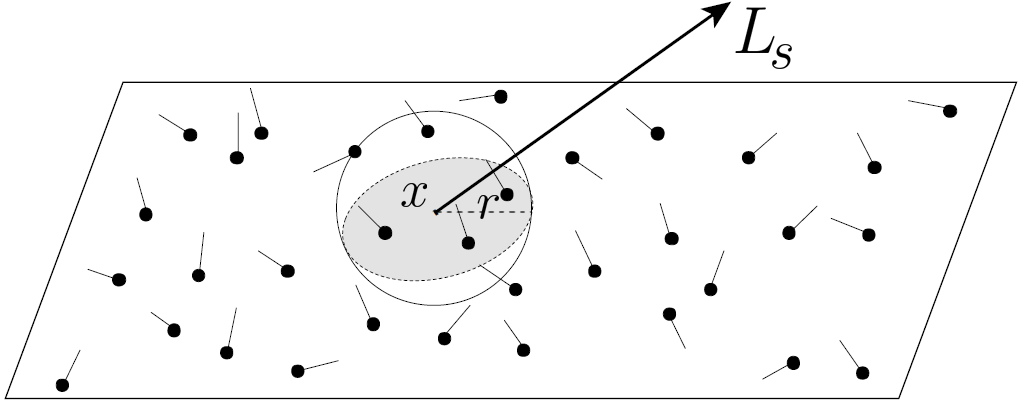
\includegraphics[width=4.0in]{img/PM-density.PNG}
	\caption[Density Estimation]{An illustration of density estimation. The process can be considered as growing a sphere until $N$ photons are located. (Image courtesy of \citeauthor{jensen1996global})}
	\label{fig:PM:densityEstimate}
\end{figure}

\subsection{Rendering}
\label{sec:PM:render:render}
Rendering is categorized into accurate computation and approximate evaluation.
This is based on how important each region is.

\subsubsection*{Accurate Computation}
For direct illumination, where human eyes can be extremely sensitive to errors, accurate computation is used.
As mentioned in section \ref{sec:PM:data:photonTracing}, no photon records are created at specular and glossy surfaces.
Thus for specular and glossy scatterings, accurate computation is used.
These situations correspond to line 6 in \textcolor{blue}{Algorithm \ref{alg:PM:secondPass}}.

\subsubsection*{Approximate Evaluation}
For scattering events between diffuse surfaces, approximate evaluation is used.
This is in fact the majority of indirect illumination.
Caustics is handled using a dedicated photon map, which will be discussed in section \ref{sec:PM:more:classes}.
This corresponds to line 4 in \textcolor{blue}{Algorithm \ref{alg:PM:secondPass}}.

\subsubsection*{Filtering}
During density estimation, illumination effects like caustics could be blurred because of the kernel density estimator nature.
This can be solved by using filtering techniques.
Two filters giving good results are the cone filter and the Gaussian filter.
The cone filter gives each photon to be used a weight according to the distance to query point.
The weight is given as
\begin{equation*}
	w_{cone} = 1- \frac{d_p}{kr}
\end{equation*}
where $k\geq 1$ is a user specified constant and $r$ is the distance to the $N$-th photon record as mentioned in equation \ref{eq:PM:densityEstimate}.

The Gaussian filter assigns weights as
\begin{equation*}
	w_{Gaussian} = \alpha \left[ 1-\frac{1-e^{-\beta \frac{d_p^2}{2r^2}}}{1-e^{-\beta}} \right]
\end{equation*}
where empirically $\alpha = 1.818$ and $\beta = 1.953$.

\section{Miscellaneous Photon Maps}
\label{sec:PM:more}
In previous sections, we discussed a na{\"i}ve way of rendering using photon maps.
In fact, photon maps can be used in many other ways.
In this section, we discuss the usage of photon maps.

\subsection{Classifying Photons}
\label{sec:PM:more:classes}
\subsubsection*{Caustics Photons}
Caustics photons are photons that arrive at diffuse surfaces after being scattered by specular or highly glossy surfaces.
Caustics effects are difficult for traditional Monte Carlo ray tracing, as shown in \figurename \ref{fig:PM:compare} (a).
Caustics effects via specular surfaces are even harder for Monte Carlo ray tracing and BDPT, as shown in \figurename \ref{fig:PM:compare} (b).
Since the way we used photon maps in previous section limits the advantage of photons, it is necessary that we dedicate a separate photon map for caustics.

To distinguish this new photon map with previously defined photon map, the new photon map containing only caustic photons is called \textit{caustic photon map} and the original photon map containing all sorts of photons is called \textit{global photon map}.
Notice we still construct the global photon map in the first pass.

To construct a caustic photon map, photons are emitted towards specular and highly glossy surfaces in the scene.
Since the caustic photon map is directly visualized to give caustic effects, we usually need higher quality than the global photon map.
During rendering, the caustic component can be separated and rendered alone.
Notice despite caustics are directly visible, we still use approximate evaluation to compute it instead of using traditional Monte Carlo ray tracing.

\subsubsection*{Shadow Photons}
As discussed in previous sections, photon records accumulated on surfaces indicate how much illumination is distributed.
It is natural to conclude that shadow regions will accumulate less photons than directly illuminated regions.
During the computation of direct illumination, shadow ray visibility tests take a big share of the computation time.
Often in a scene, regions are either fully illuminated or fully in shadow.
The penumbra regions are usually limited.
Based on this observation, we would like to take advantage of photon maps and distinguish penumbra regions from fully illuminated and fully shadowed regions.

Shadow photons are extensions to regular photons.
Unlike regular photons records, a shadow photon record is created by tracing photons through all geometries in the scene without scattering, and only create record after first intersections.
Each shadow photon should be given a flag indicating the light source from which it is emitted and a flag indicating that it is a shadow photon.
The creation of shadow photons is illustrated in \figurename \ref{fig:PM:shadowPhoton}.

\begin{figure}
	\centering
	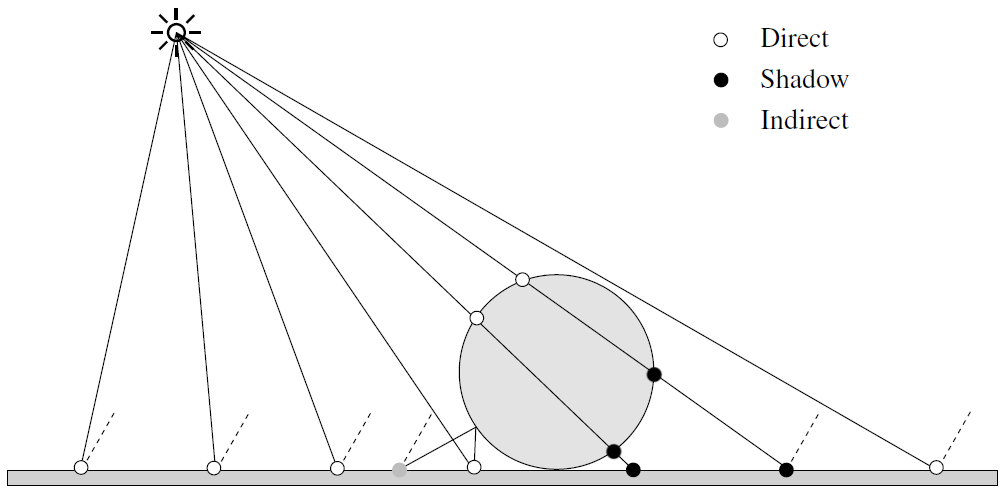
\includegraphics[width=4.0in]{img/PM-shadowPhoton.png}
	\caption[Shadow Photon Creation]{Shadow photon records are created by tracing photons from lights through all geometries without scattering. Only events after first intersections create shadow photon records. (Image courtesy of \citeauthor{jensen1995photon})}
	\label{fig:PM:shadowPhoton}
\end{figure}

Recall that for direct illumination and specular-reflected/refracted illumination we are still using Monte Carlo ray tracing.
The only region that a shadow ray pays off is in the penumbra region.
To exploit shadow photons, we simply gather few photon records like we did in density estimation.
If all of them are direct illuminated photon records, this region is very likely to be a directly illuminated region.
If all of them are shadow photons, this region is for sure a shadow region.
If a combination of direct illuminated photon records and shadow photon records happens, this region is then a penumbra region, and we can start tracing shadow rays.

\subsection{Working with Irradiance Caching}
\label{sec:PM:more:withIC}
Both irradiance caching and photon mapping are trying to cache illumination information before real rendering.
\citeauthor{christensen1999faster} observed that many photon map query for diffuse inter-reflections in the rendering pass of photon mapping can be simplified by precomputing irradiance values at photon records \cite{christensen1999faster}.

As we know from the previous chapter, the computation of irradiance value can be costly.
A photon map usually contains millions of photon records, thus it is impractical to compute irradiance value for all photon records.
\citeauthor{christensen1999faster} proposed to only compute for a selected set of all photon records.

Selected photon records are augmented with a computed irradiance value and surface normal information.
During the rendering phase, only the nearest photon record with precomputed irradiance value is needed.
To make results more accurate, it is better to select a record with similar surface normal as the query point.
The results rendered with this technique is shown in \figurename \ref{fig:PM:PMIC}.

\begin{figure}[!ht]
	\begin{subfigure}{0.24\textwidth}
		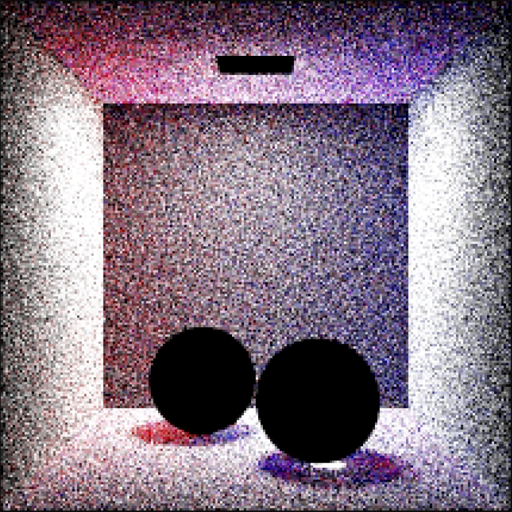
\includegraphics[height=1.4in]{img/PM-PMIC-0.png}
		\caption{ }
	\end{subfigure}%
	~
	\begin{subfigure}{0.24\textwidth}
		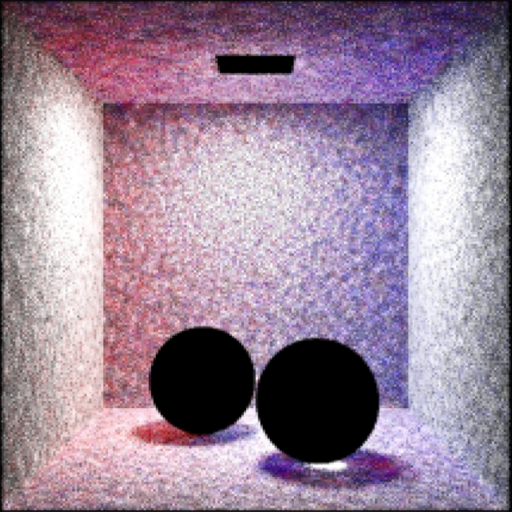
\includegraphics[height=1.4in]{img/PM-PMIC-1.png}
		\caption{ }
	\end{subfigure}%
	~
	\begin{subfigure}{0.24\textwidth}
		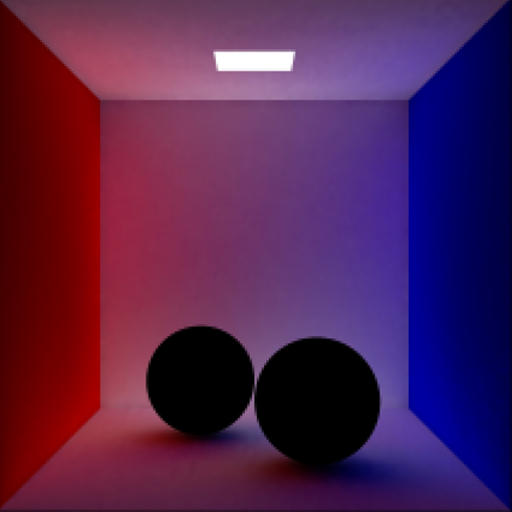
\includegraphics[height=1.4in]{img/PM-PMIC-2.png}
		\caption{ }
	\end{subfigure}%
	~
	\begin{subfigure}{0.24\textwidth}
		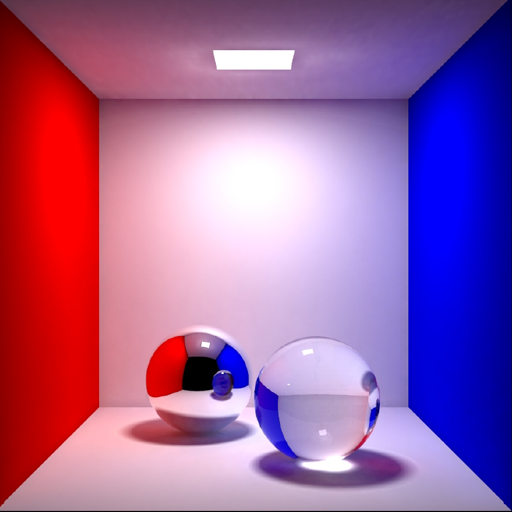
\includegraphics[height=1.4in]{img/PM-PMIC-3.png}
		\caption{ }
	\end{subfigure}
	\caption[Photon Mapping and Irradiance Caching]{The Cornell box scene rendered using photon mapping with precomputed irradiance. (a) Visualization of the global photon map. (b) Visualization of precomputed irradiance. (c) Soft indirect illumination term. (d) Final render with global illumination. (Images courtesy of \citeauthor{christensen1999faster})}
	\label{fig:PM:PMIC}
\end{figure}

\subsection{Working as Importance}
\label{sec:PM:more:importance}
As we discussed in section \ref{sec:GI:formulation:MC}, it is almost impossible to get the optimal distribution to importance sample a function without any \textit{a priori} knowledge of the function.
With photon mapping, we are distributing illumination information across the scene, and cache the information in a data structure.
Intuitively, this information can be exploited as a guidance.
Recall in section \ref{sec:GI:formulation}, where we solve the integral in the rendering equation
\begin{gather*}
\begin{aligned}
	L_s &= \int_{\Omega_x} f_s(\Theta, x, \omega) L(x \leftarrow \omega) \left| \cos (N_x, \omega) \right| d\omega \\
	&= \int_{\Omega_x} \frac{f_s(\Theta, x, \omega) L(x \leftarrow \omega) \left| \cos (N_x, \omega) \right|}{p(x, \omega)} p(x, \omega) d\omega
\end{aligned}    
\end{gather*}
using a Monte Carlo estimator
\begin{gather*}
\begin{aligned}
	\widehat{L}_s &= \frac{1}{N} \sum_{i=1}^{N} \frac{f_s(\Theta, x, \omega_i) L(x \leftarrow \omega_i) \left| \cos (N_x, \omega_i) \right|}{p(x, \omega_i)}\\
	&= \frac{1}{N} \sum_{i=1}^{N} \frac{f_s(\Theta, x, \omega_i) d^2 \Phi(x, \omega_i) / dA}{p(x, \omega_i)}.
\end{aligned}
\end{gather*}

Notice the equations are given in a flux-based formulation, which is what a photon map can provide.
To importance sample this integral, the PDF is ideally
\begin{equation}
\label{eq:PM:importance}
	p(x, \omega) \propto \frac{f_s(\Theta, x, \omega) d^2 \Phi(x, \omega)}{dA}.
\end{equation}

With this formulation, it is now clear that the photon map we calculated can work as an \textit{a priori} knowledge to guide sampling.
\citeauthor{jensen1995importance} first proposed to use pre-calculated photon map as an importance sampling guidance \cite{jensen1995importance}.
To exploit photon map in importance sampling, BSDF and flux information need to be jointly sampled.
A simple way to sample flux information by \citeauthor{jensen1995importance} is to stratify the hemisphere into cells, and build a histogram containing flux information.
By uniformly sampling the cumulative histogram, we can easily get an importance sampled direction according to flux information.
\figurename \ref{fig:PM:importance} gives a comparison of traditional path tracing and photon map driven importance sampled path tracing.

\begin{figure}[b]
	\centering
	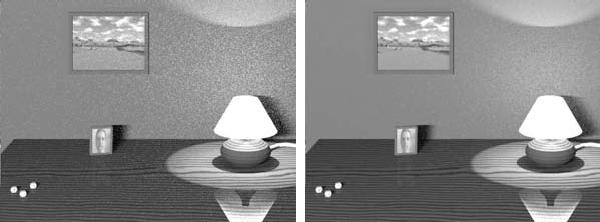
\includegraphics[width=4.5in]{img/PM-importance.png}
	\caption[Photon Driven Importance Sampling]{Left: traditional path tracing. Right: path tracing with photon map driven importance sampling. Notice the obvious variance reduction. (Images courtesy of \citeauthor{jensen1995importance})}
	\label{fig:PM:importance}
\end{figure}

%%%%%%%%%%%%%%%%%%%%%%%%%%%%%%%%%%%%%%%%%%%%%%%%%%%%%%%%%%%%%%%%%%%%%%%%%%%%%%%%%%%%%%%%%%%%%%%%%%%%%%%%%%%%%%%%%%%%%%%%%%%%%%%%%%%%%%%%%%%%%%%%%%%%%%%%%%%%

\chapter{Visibility Caching}
\label{chap:vis_cache}

\begin{figure}[!ht]
	\begin{subfigure}{0.30\textwidth}
		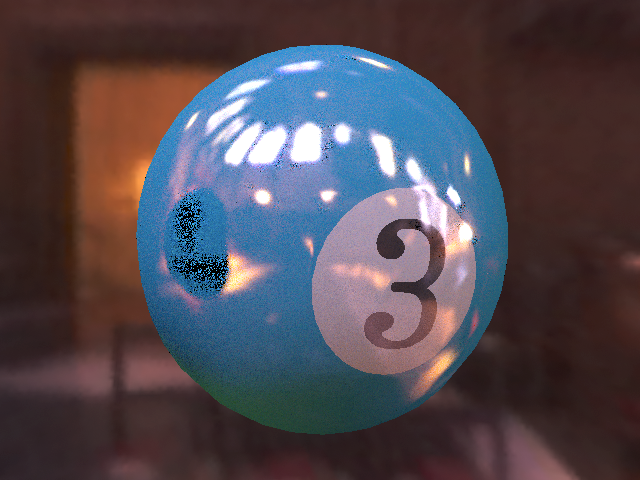
\includegraphics[height=1.37in]{img/VC-0-variance.png}
		\caption{Variance due to visibility}
	\end{subfigure}%
	~
	\begin{subfigure}{0.38\textwidth}
		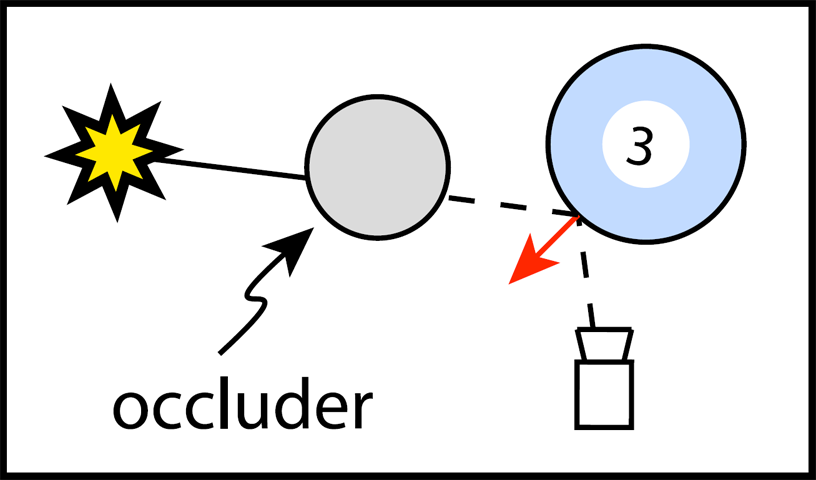
\includegraphics[height=1.37in]{img/VC-0-scene.png}
		\caption{Scene setup}
	\end{subfigure}%
	~
	\begin{subfigure}{0.30\textwidth}
		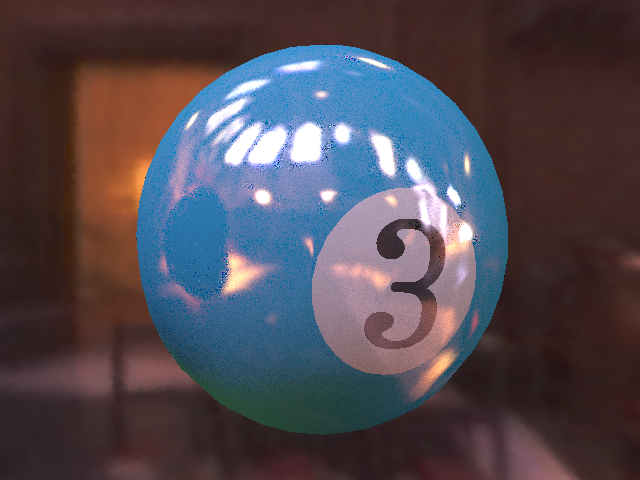
\includegraphics[height=1.37in]{img/VC-0-reference.png}
		\caption{Reference}
	\end{subfigure}
	\caption[Variance Due to Visibility]{Variance caused by visibility. (a) Variance can be obviously seen in the reflection part, where a light source is occluded by another object. (b) The scene setup for the render. (c) The reference image. Notice the difference in corresponding part. (Images courtesy of \citeauthor{clarberg2008VisCorrelation})}
	\label{fig:VC:intro}
\end{figure}

\lettrine{R}{ecall} in previous chapters, all we did was working around the rendering equation.
In irradiance caching, we cache the incoming radiance from all directions, which corresponds to the term $\int L(x \leftarrow \omega) \left| \cos (N_x, \omega) \right| d\omega$ in equation \ref{eq:renderEquation:hemisphere}.
In radiance caching, with similar spirit as in irradiance caching, we cache incoming radiance as well as incoming distribution, which makes radiance caching compatible with glossy surfaces.
In photon mapping, we work with a Radiosity spirit and use photons to solve the flux term in equation \ref{eq:PM:formulation}, which is an equivalent expression of the rendering equation in another form.

With slight reference to equation \ref{eq:renderEquation:threePoint}, we can find that visibility, as a non-deterministic term, is not exploited yet.
On the one hand, in real situations, visibility does introduce variance.
Imagine for example in a penumbra region, we sample a point on a light source.
The chances are that the sample point on the light source is occluded.
In this case, a black pixel will be returned if no further actions are taken.
\figurename \ref{fig:VC:intro} shows one such situation.

On the other hand, visibility tests are expensive.
Usually in ray tracing, an accompany acceleration structure is built to accelerate ray-object intersections.
To find intersections, a ray must be traversed through the acceleration structure.
Rays are categorized into \textit{intersection rays} and \textit{shadow rays}, and corresponding intersections are called \textit{closest hit} and \textit{any hit} \cite{smits2005efficiency}.
Intersection rays contribute by providing critical information that the rendering equation need and can not be simplified.
Shadow rays, recall in section \ref{sec:PM:more:classes}, tend to show correlation.
According to many research, shadow rays take up a significant portion of all rays.

In this chapter, we discuss visibility caching, which aims at the visibility term in the rendering equation.
Visibility caching is not as old as previous schemes, and still maturing.
In section \ref{sec:VC:vTerm} we present situations where visibility tests are used.
We study the correlation of visibility in section \ref{sec:VC:correlation}, which provides theoretical premise for following content.
We discuss ways to represent visibility in section \ref{sec:VC:represent}.
Section \ref{sec:VC:structure} is about the data structure to hold visibility caches.
We discuss different ways of using visibility caches in section \ref{sec:VC:render}.

\section{Visibility Tests}
\label{sec:VC:vTerm}
As just mentioned, visibility tests are shadow ray queries in the acceleration structure.
A shadow ray is a ray formed by two fixed points.
The input of a visibility test is a shadow ray $r_s(\mathbf{o}, \vec{d}, t_0)$ with a fixed starting point $\mathbf{o}$ and a finite and fixed $t_0$ value in direction $\vec{d}$.
If during the acceleration structure traversal, there is any hit that gives a smaller $t$ value than $t_0$, then shadow ray $r_s$ is occluded and two points are not mutually visible.
The output of a visibility test is thus a boolean value.

The above process in the pre-ray tracing era is handled by the \textit{z-buffer} technique in rasterization.

\subsection{Sampling Lights}
\label{sec:VC:vTerm:sampleLight}
Visibility tests can happen in many situations in the scope of rendering.
One of the major situation is in sampling lights.
In fact this is the situation where it gets the name \textit{shadow ray}.
In traditional ray tracing, we cast a shadow ray to a light source to determine if a point is in shadow region.
In unidirectional path tracing with \textit{next event estimation}, we not only sample the BSDF, but also lights, see \figurename \ref{fig:GI:MIS}.
In \textit{many-light rendering}, shadow rays connect shading points to VPLs, see section \ref{sec:imp_cache:algorithm:IR}.

\subsection{Connecting Vertices in BDPT}
\label{sec:VC:vTerm:BDPT}
In BDPT, for each sample within a pixel, two sub-paths are generated.
An eye sub-path $\{p_1, p_2, \dots p_x\}$ and a light sub-path $\{q_y, \dots q_1, q_0\}$ are constructed from the camera and a light source with length $x$ and $y$ respectively, where $p_i$ is an eye sub-path vertex and $q_j$ is a light sub-path vertex.

To construct a final path that connects the eye sub-path and the light sub-path, visibilities between vertices from two sides are tested and the contribution of each connection strategy is combined using MIS (see section \ref{sec:GI:trend}).
In some literature, these rays are referred to as \textit{visibility rays} to better describe their functionality and distinguish them from shadow rays.
This process is shown in \figurename \ref{fig:VC:visTest:bdpt}.

\begin{figure}
	\centering
	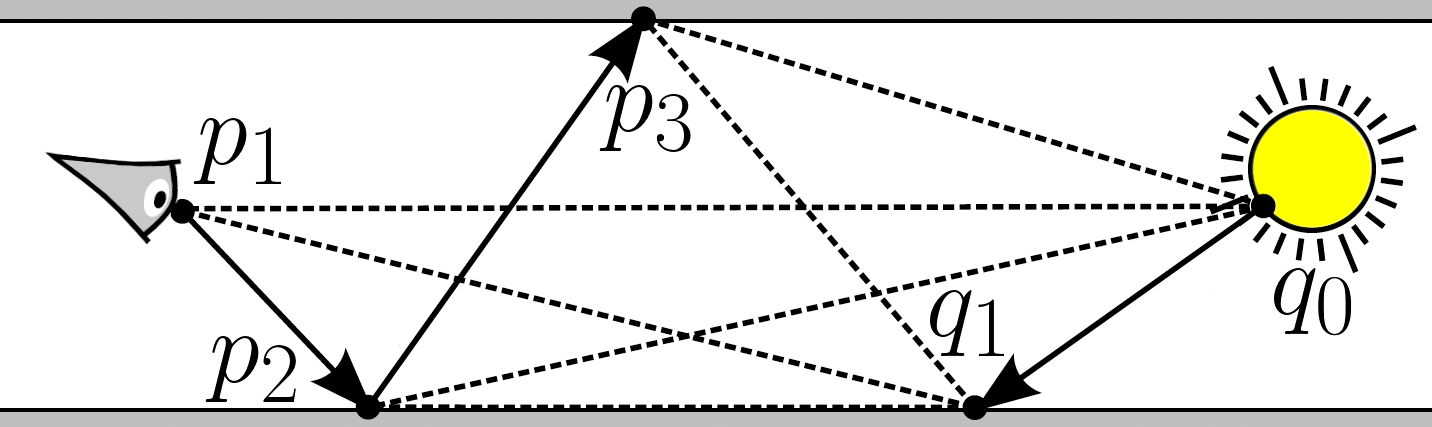
\includegraphics[width=3.0in]{img/VC-1-BDPT.png}
	\caption[Visibility Tests in BDPT]{An illustration of visibility tests in BDPT. A eye sub-path of length $3$ and a light sub-path of length $2$. Dotted lines mean the visibility tests.}
	\label{fig:VC:visTest:bdpt}
\end{figure}

\section{Visibility Correlation}
\label{sec:VC:correlation}
Recall in section \ref{sec:PM:more:classes}, where we introduced shadow photons.
Intuitively, a significant portion of scene surfaces share similar hemispherical visibility with their vicinity.
In \citeyear{clarberg2008VisCorrelation}, \citeauthor{clarberg2008VisCorrelation} measured visibility correlation and proposed a robust algorithm to exploit this correlation \cite{clarberg2008VisCorrelation}.
There are mainly three components that are affecting visibility correlation, viz.\ distance, normal difference and surface offset, as shown below.

\begin{figure}[!ht]
	\begin{subfigure}{0.33\textwidth}
		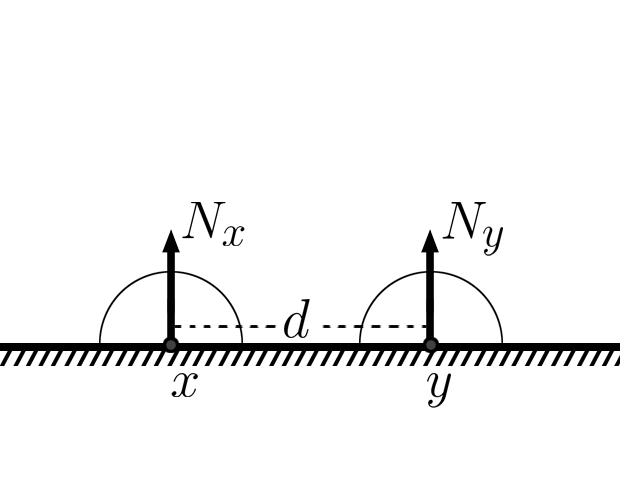
\includegraphics[height=1.4in]{img/VC-2-distance.png}
		\caption{Distance}
	\end{subfigure}%
	~
	\begin{subfigure}{0.33\textwidth}
		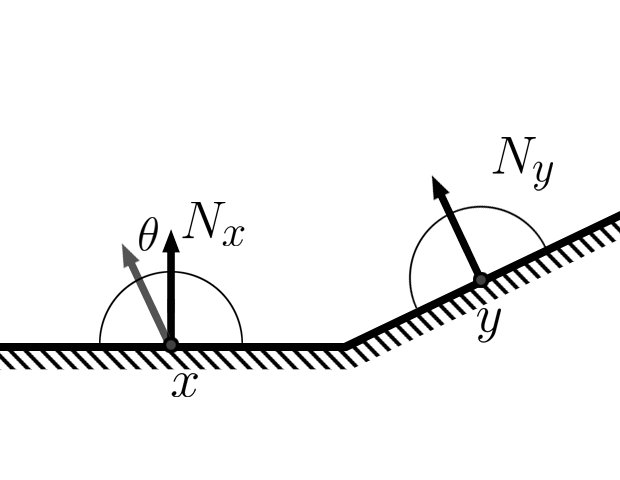
\includegraphics[height=1.4in]{img/VC-2-normal.png}
		\caption{Normal difference}
	\end{subfigure}%
	~
	\begin{subfigure}{0.33\textwidth}
		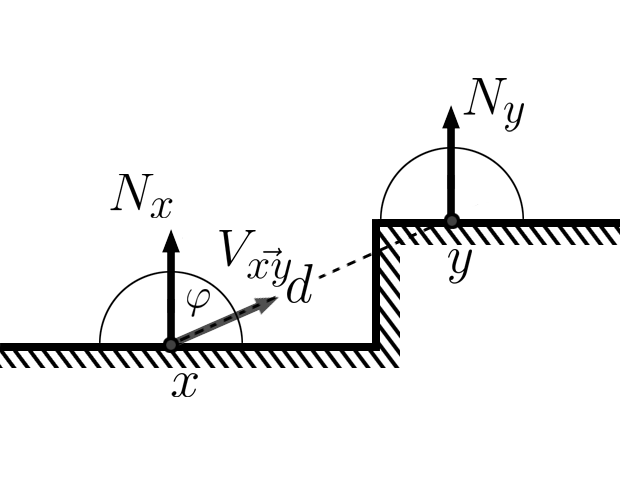
\includegraphics[height=1.4in]{img/VC-2-displace.png}
		\caption{Surface offset}
	\end{subfigure}%
\end{figure}

\citeauthor{clarberg2008VisCorrelation} setup experiments measuring the relationship between average correlation as a function of distance and normal difference $\bar{\rho}(d, \theta)$.
During the experiments, environmental light is used so that an outgoing direction $\omega$ can be used to indicate illumination from the same light source, i.e.\ at point $x$ and $y$, if $V_x(x, \omega) = V_y(y, \omega)$, point $x$ and $y$ are receiving same illumination from direction $\omega$.
The results of one example scene from \cite{clarberg2008VisCorrelation} are shown in \figurename \ref{fig:VC:correlation}.

\begin{figure}
	\begin{subfigure}{0.5\textwidth}
		\centering
		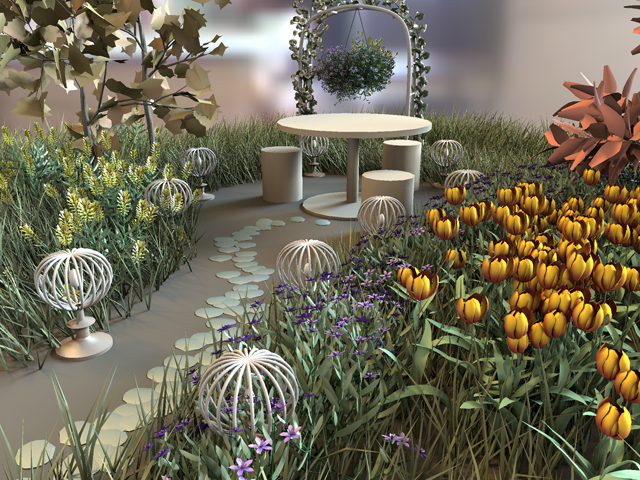
\includegraphics[height=1.7in]{img/VC-2-correlate1.png}
		\caption{The \textit{garden} scene}
	\end{subfigure}%
	\begin{subfigure}{0.5\textwidth}
		\centering
		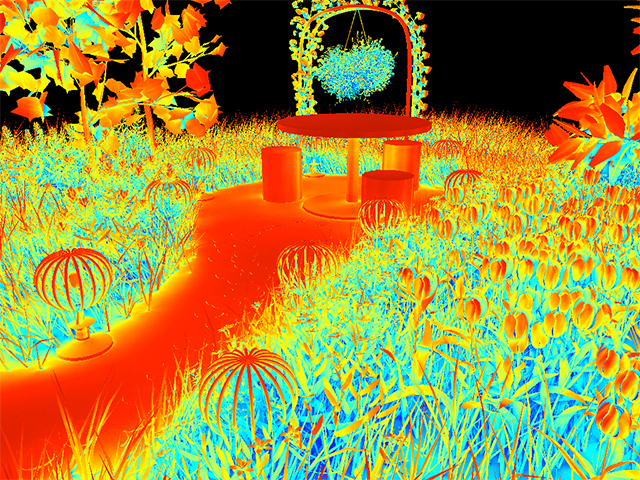
\includegraphics[height=1.7in]{img/VC-2-correlate2.png}
		\caption{Visibility correlation visualization}
	\end{subfigure}
	
	\begin{subfigure}{1.\textwidth}
		\centering
		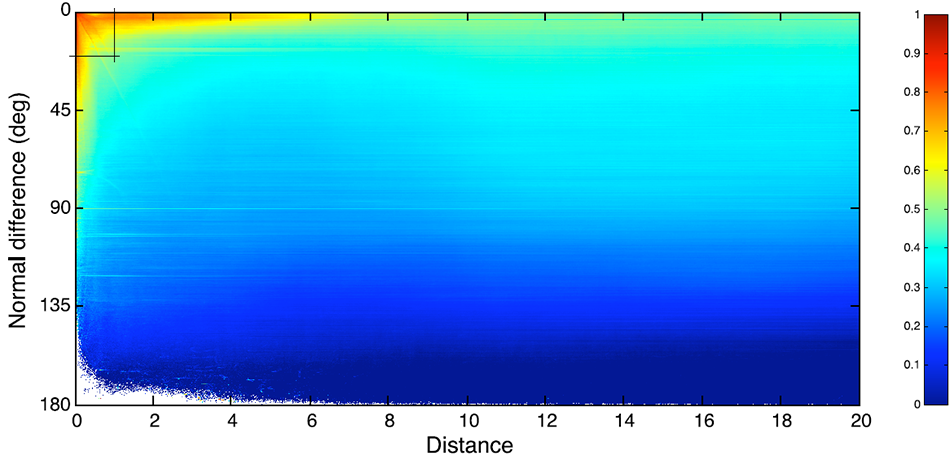
\includegraphics[height=2.5in]{img/VC-2-correlate3.png}
	\end{subfigure}
	\caption[Visibility Correlation]{Visibility correlation in a complex scene. Scene: the \textit{garden}. The average correlation is a function of distance and normal difference. The results are clamped to $\left[ 0, 1\right]$, where $1$ means strongly positively correlated, $0$ means not correlated. (Images courtesy of \citeauthor{clarberg2008VisCorrelation})}
	\label{fig:VC:correlation}
\end{figure}

As can be seen from the results, visibility is often highly correlated over large smooth surfaces \cite{clarberg2008VisCorrelation}.
For flat areas like the walk path on the ground, correlation is very strong, while for complex areas like the grass, correlation is negligible.
Thus it is possible to exploit this correlation in global illumination.

\section{Visibility Representation}
\label{sec:VC:represent}
Visibility is extremely direction dependent, thus we need a representation that preserves directional information.
Intuitively, the starting point is the upper or lower hemisphere, or full sphere when participating media exists.

Another representation is point-point mutual visibility.
However, this representation require huge amount of memory and expensive lookups, especially as scene grows complex.

In this section we present several visibility representations, which are mostly based on hemi-spherical or spherical visibility.

\subsection{Shadow Maps}
\label{sec:VC:represent:SM}
\textit{Shadow map} is originally used to determine if a point in scene is lit by a specific light source.
The method was proposed by \citeauthor{williams1978SM} in \citeyear{williams1978SM} \cite{williams1978SM}.
Shadow maps and its variants are considered to be the \textit{de facto} standard technique to solve shadow problems in rasterization.

The observation that shadow mapping based on is the fact that every point visible from a light is lit by the light, and those invisible lie in the shadow region of this light.
This observation does not take specular surfaces into consideration, which makes sense because in rasterization reflections and refractions are not solved the way we solve them in ray tracing.
The process of creating a shadow map is conceptually simple, a point on the light source is used as a view point, then the scene seen from this viewpoint is rendered to an image.
This can be a unidirectional view, or a omni directional view, with difference being the opening angle of the view frustum.

The scene is not rendered as a full colored representation to the viewpoint, but a map of depth values, i.e.\ distance of visible point to the view point.
When using this shadow map during rendering, the distance to the light source from the point to be shaded is checked and compare to the depth value stored in corresponding pixel of the shadow map.
This process is illustrated in \figurename \ref{fig:VC:shadowMaps}.
For more details of shadow mapping techniques, refer to the original paper \cite{williams1978SM} and the book \citetitle{eisemann2011real} \cite{eisemann2011real}.

\begin{figure}
	\centering
	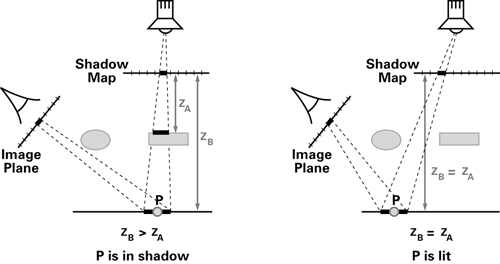
\includegraphics[width=4.0in]{img/VC-3-shadowMap.png}
	\caption[Shadow Mapping]{An illustration of shading with shadow map. Left: depth value of point \textbf{p} from the light source is larger than the stored value in corresponding SM pixel, thus in shadow. Right: depth value of point \textbf{p} from the light source equals stored value in corresponding shadow map pixel, thus lit. (Images courtesy of NVIDIA)}
	\label{fig:VC:shadowMaps}
\end{figure}

The depth value corresponds to the $t$ value of a ray in ray tracing, which is a very convenient coincidence.
We can use shadow maps with the same spirit and render the (hemi-)spherical view of the scene into depth/distance values.
For this step, we can use multiple techniques.
Rasterization can be fast for its efficient hardware implementation.
Ray casting, on the other hand, provides similar results but less rapid.
Since all we need for this visibility shadow map is the depth/distance value of direct visible surface points, rasterization is a good option, as is the case in \cite{ulbrich2013progressive}.

The pseudo code for creating visibility caches using shadow map as visibility representation is shown in \textcolor{blue}{Algorithm} \ref{alg:VC:createCache}.
The procedure \textsc{DistributePoints} shares same spirit as the pre-pass in (ir)radiance caching and photon mapping.
Records are only created at non-specular surfaces.
The procedure \textsc{RenderDepth} renders the corresponding view into a shadow map, either a rasterizer or a ray caster can be used here .

\begin{algorithm}
\caption[Create Visibility Caches]{Pseudo code to create visibility caches}
\addtocontents{loa}{\vskip 4pt}
\label{alg:VC:createCache}
\begin{algorithmic}[1]
	\Procedure{CreateVisCache}{$\mathbf{scene}$, \textbf{visibilityMap}}
		\State $\mathbf{P} \gets$ \textsc{DistributePoints}($\mathbf{scene}$, \textit{non-specular})
		\ForAll{$\mathbf{p}_i$ in $\mathbf{P}$}
			\State $r_i \gets \varnothing$
			\State $r_i.p \gets \mathbf{p}_i$
			\State $r_i.n \gets \mathbf{p}_i.n$
			\If{$\mathbf{p}$ in participating media}
				\State $r_i.map \gets$ \textsc{RenderDepth}($\mathbf{p}_i$, \textit{sphereical-view})
			\Else
				\State $r_i.map \gets$ \textsc{RenderDepth}($\mathbf{p}_i$, \textit{hemisphereical-view})
			\EndIf
			\State Store $r_i$ in \textbf{visibilityMap}
		\EndFor
	\EndProcedure
\end{algorithmic}
\end{algorithm}

\subsection{Variants of Shadow Maps and Others}
\label{sec:VC:represent:xSMs}

\subsubsection*{Imperfect Shadow Maps}
\textit{Imperfect Shadow Maps} (ISM), is a technique proposed by \citeauthor{ritschel2008ISM} to work with VPL based global illumination algorithms \cite{ritschel2008ISM}.
VPL based instant radiosity methods, as global illumination techniques using rasterization, benefit greatly from hardware implementations.
Despite this advantage, it is still impractical to render a regular shadow map for each VPL.
On the one hand, accurate visibility is not necessary for indirect illumination to be physically plausible.
On the other hand, a regular shadow map for each VPL is inefficient both memory-wise and lookup-wise.

In short, an ISM is a low resolution shadow map, e.g.\ $32\times 32$.
The core idea is to distribute a point set to crudely represent the scene.
The points in the point set are VPLs.
For each point in the point set, an ISM is rendered and later used to approximate visibility in the indirect illumination computation.

Though initially proposed to solve indirect illumination, where for many applications accurate visibility is not necessary to produce physically plausible images, ISMs are used for direct illumination as well.
This will introduce obvious errors, such as holes, due to its low resolution.
This problem is solved by using a pull-push correction.
An example scene rendered with ISM is shown in \figurename \ref{fig:VC:ISM}.

\begin{figure}
	\centering
	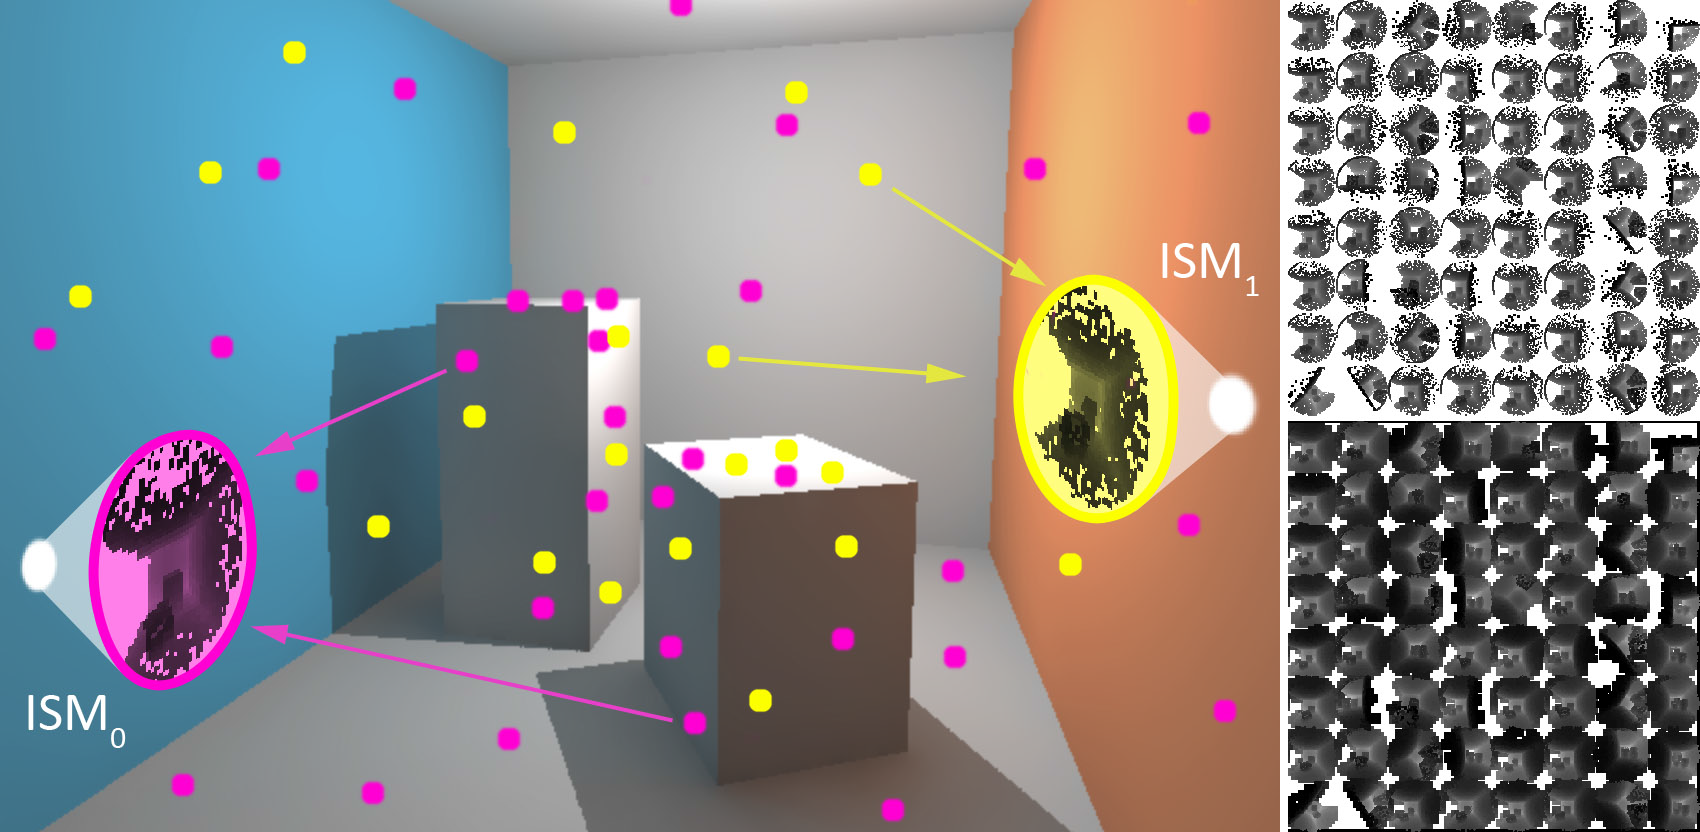
\includegraphics[width=4.0in]{img/VC-3-ISM.png}
	\caption[Imperfect Shadow Maps]{A scene rendered using imperfect shadow maps. Two ISMs are shown as a demonstration in the left image, with corresponding colored dots contributing to the ISM. All ISMs used are shown to the right, with the top image presenting ISMs rendered without pull-push, the bottom image with pull-push. (Images courtesy of \citeauthor{ritschel2008ISM})}
	\label{fig:VC:ISM}
\end{figure}

There are many improvements toward ISM.
\citeauthor{ritschel2011making} makes ISM view adaptive by placing more sample points near camera viewpoint, instead of uniformly distribute samples through out the scene \cite{ritschel2011making}.
\citeauthor{hollander2011ManyLODs} proposed a \textit{ManyLoDs} algorithm to compute desired data, e.g.\ a shadow map, from many views using the scene acceleration structure \cite{hollander2011ManyLODs}.
The process resembles a node cut style traversal scheme, like the \textit{light cuts} algorithm.
This improvement is more beneficial for GPUs where many ISMs need to be computed in parallel.

\subsubsection*{Octahedral Representation}
Other than regular (hemi)spherical representations, octahedral map is also frequently used to represent data.
\citeauthor{von2016efficient} use an octahedral map to represent visibility in volume rendering \cite{von2016efficient}, where a visibility grid is set up and in each of the eight faces, a sweeping plane algorithm is used to sweep through all grids and accumulate the visibility throughput.
Both the use of octahedral map and sweeping scheme make the algorithm efficient for their case.
An example of octahedral map is shown in \figurename \ref{fig:VC:octahedra}.

\begin{figure}[t]
	\begin{subfigure}{0.5\textwidth}
		\centering
		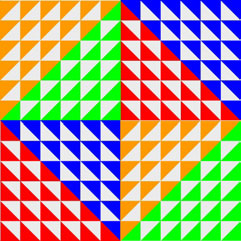
\includegraphics[height=1.2in]{img/VC-3-octa-1.png}
		\caption{A 2D representation of an octahedral map}
	\end{subfigure}%
		\begin{subfigure}{0.5\textwidth}
		\centering
		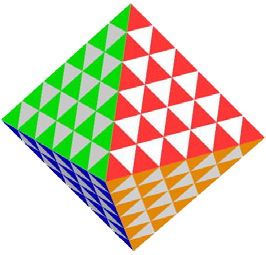
\includegraphics[height=1.2in]{img/VC-3-octa-2.png}
		\caption{The octahedral map in 3D view}
	\end{subfigure}
	\caption[Octehadral Maps]{An example of octahedral map.}
	\label{fig:VC:octahedra}
\end{figure}

\subsubsection*{Cluster-based Representation}
\citeauthor{popov2013adaptive} proposed to cluster scene surfaces and use inter-cluster visibility to approximate the point-point visibility tests \cite{popov2013adaptive}.
The assumption is that points belong to the same cluster share exactly same visibility.
A hash map is used to store cluster caches.
The scheme is shown in \figurename \ref{fig:VC:cluster}.

\begin{figure}[b]
	\centering
	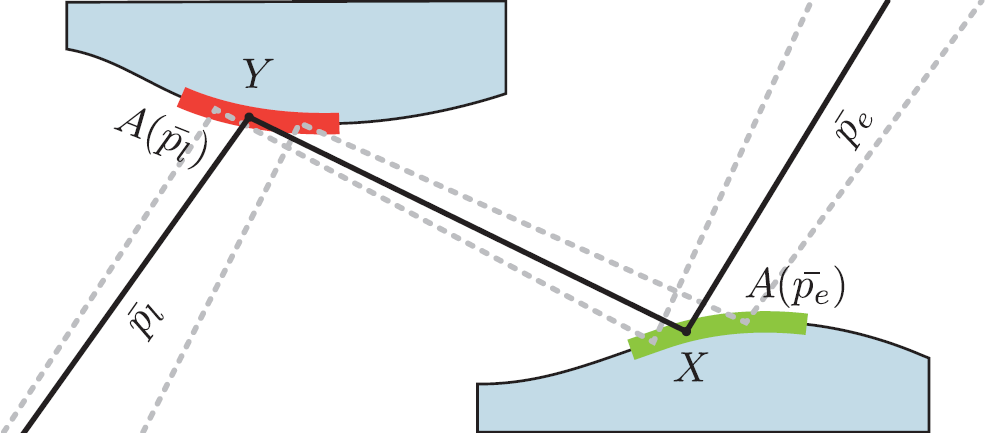
\includegraphics[width=3.0in]{img/VC-3-cluster.png}
	\caption[Clustered Visibility]{Paths containing vertices in the same clusters share same visibility. (Image courtesy of \citeauthor{popov2013adaptive})}
	\label{fig:VC:cluster}
\end{figure}

\section{Visibility Query Structure}
\label{sec:VC:structure}
Recall in previous chapters, where we talked about requirements for a data structure to be eligible.
For the case of visibility caches, we still face the same issue.
Thus, from the experience of previous caching techniques, the suitable data structure for visibility caching is a \textit{k}-d tree.

\section{Using the Visibility Cache}
\label{sec:VC:render}
When using the visibility cache, we are again facing the problem when we did with photon mapping: whether we want to directly use the cache in the computation or we want to use it as a guidance for importance sampling.
For direct illumination, the scheme we represent and cache the visibility would not benefit much since we are not using rasterization during rendering.
For indirect illumination, as mentioned previously, visibility can be approximated by interpolating caches.

\subsection{Indirect Illumination}
\label{sec:VC:render:indirect}
To use visibility cache, we need to restrict usable caches to be within a certain range.
In other words, we need to use the scheme of irradiance caching to locate cache records within an acceptable range, instead of the scheme of photon mapping.

When we have the records, we need to assign each record a weight according to the distance, normal difference and displacement.
With slight reference to the illustrations in section \ref{sec:VC:correlation} ,the weight function is given by
\begin{equation}
	w(x,y) = \left(1-\frac{\textup{arccos}(\left|N_x\cdot N_y\right|)}{\pi}\right)\left( 1-\frac{d/d_{max}}{1+5d/d_{max}} \right ) \sqrt{1-\left|N_x \cdot V_{\vec{xy}} \right|}
\end{equation}
where:
\begin{itemize}
	\item[-] $1-\frac{\textup{arccos}(\left|N_x\cdot N_y\right|)}{\pi}$ is the normal difference
	\item[-] $1-\frac{d/d_{max}}{1+5d/d_{max}}$ is the spatial difference, where $d$ is the distance between point $x$ and $y$
	\item[-] $\sqrt{1-\left|N_x \cdot V_{\vec{xy}} \right|}$ is the surface offset, $V_{\vec{xy}}$ is the unit vector pointing from $x$ to $y$.
\end{itemize}

The process of using the visibility cache for visibility approximation is shown in \figurename \ref{fig:VC:useCache} and \textcolor{blue}{Algorithm} \ref{alg:VC:useCache}.
Notice that the returned value is an weighted average of distance.
The rest of the rendering process is identical to whatever techniques applicable and will not be repeated here.

\begin{figure}[t]
	\centering
	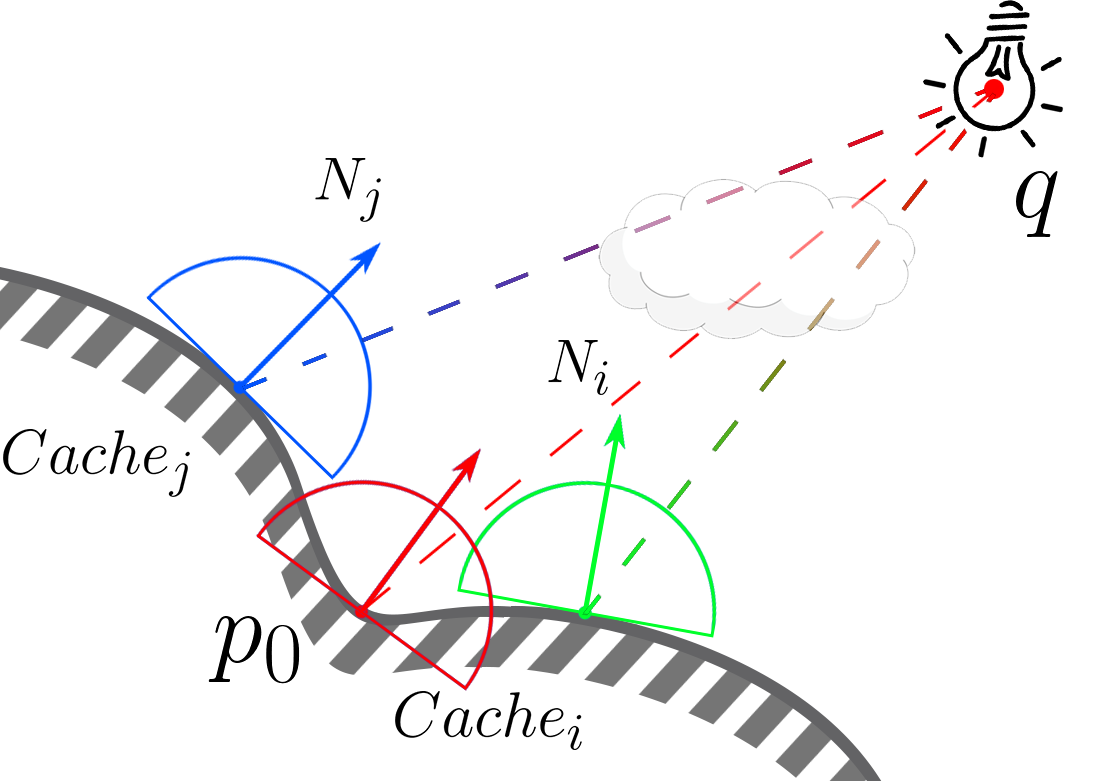
\includegraphics[width=2.5in]{img/VC-3-query.png}
	\caption[Use Visbility Cache]{An illustration of using the visibility cache. For query point $\mathbf{p}_0$ and $\mathbf{q}$, two cache records $Cache_i$ and $Cache_j$ are located. The approximated visibility is returned as the weighted sum of results from $Cache_i$ and $Cache_j$.}
	\label{fig:VC:useCache}
\end{figure}

\begin{algorithm}
	\caption[Use Visibility Caches]{Pseudo code to use visibility caches}
	\addtocontents{loa}{\vskip 12pt}
	\label{alg:VC:useCache}
	\begin{algorithmic}[1]
		\Procedure{UseVisCache}{$\mathbf{p}_0$, $\mathbf{q}$, \textbf{visibilityMap}}
		\State $\mathbf{P} \gets$ \textsc{LocateRecords}($\mathbf{p}_0$)
		\State $V\gets 0$
		\ForAll{$\mathbf{p}_i$ in $\mathbf{P}$}
		\State $w_i \gets$ \textsc{WeightRecord}($\mathbf{p}_0$, $\mathbf{p}_i$)
		\State $v_i\gets$ \textsc{QueryMap}($\mathbf{p}_i.map$, $\mathbf{q}$) 
		\State $V\mathrel{{+}{=}}v_i\times w_i$
		\EndFor
		\State \Return $V$
		\EndProcedure
	\end{algorithmic}
\end{algorithm}

\subsection{Direct Illumination}
\label{sec:VC:render:direct}
\citeauthor{clarberg2008VisCorrelation} uses \textit{control variates} technique to formulate the rendering equation with the cached visibility as a control variable.
As we discovered in section \ref{sec:VC:correlation} that visibility correlation does exist, the following equation can be formulated
\begin{gather*}
\begin{aligned}
	\widehat{L}_o &= \frac{1}{N} \sum_{i=1}^{N}\frac{L_i f_s G V}{p(\omega_i)} \\
	&= \frac{1}{N} \sum_{i=1}^{N}\frac{L_i f_s G V - \alpha L_i f_s G \widetilde{V}}{p(\omega_i)} + \alpha \int L_i f_s G \widetilde{V} d\omega
\end{aligned}
\end{gather*}
where  $\widetilde{V}$ is the approximated visibility term using the visibility cache.
This estimator is unbiased.
If $V$ and $\widetilde{V}$ are indeed correlated, this estimator will cause no more, if no less, variance than the original one.

To exploit this feature, the core idea is to augment the lighting-reflection product sampling and perform lighting-visibility-reflection joint sampling, i.e.\ $p \propto L_i f_s G \widetilde{V}$.
\citeauthor{clarberg2008VisCorrelation} uses environmental maps as light source, which makes this joint sampling more practical than with unstructured lights.
This reduces variance as expected, refer to \cite{clarberg2008VisCorrelation} for more details.
%%%%%%%%%%%%%%%%%%%%%%%%%%%%%%%%%%%%%%%%%%%%%%%%%%%%%%%%%%%%%%%%%%%%%%%%%%%%%%%%%%%%%%%%%%%%%%%%%%%%%%%%%%%%%%%%%%%%%%%%%%%%%%%%%%%%%%%%%%%%%%%%%%%%%%%%%%%%

\chapter{Importance Caching}
\label{chap:imp_cache}

\begin{figure}[!ht]
	\begin{subfigure}{0.5\textwidth}
		\centering
		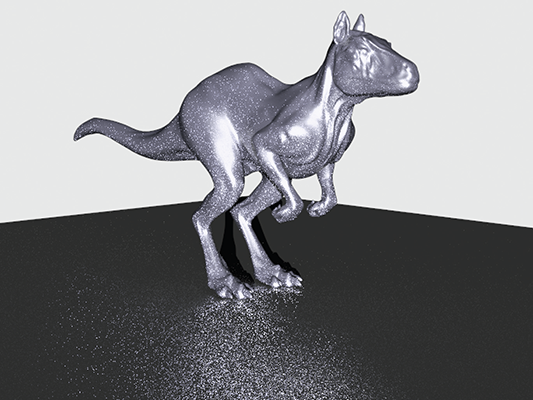
\includegraphics[height=2.2in]{img/IMP_0-1.png}
		\caption{Uniform sampling the hemisphere}
	\end{subfigure}%
	\begin{subfigure}{0.5\textwidth}
		\centering
		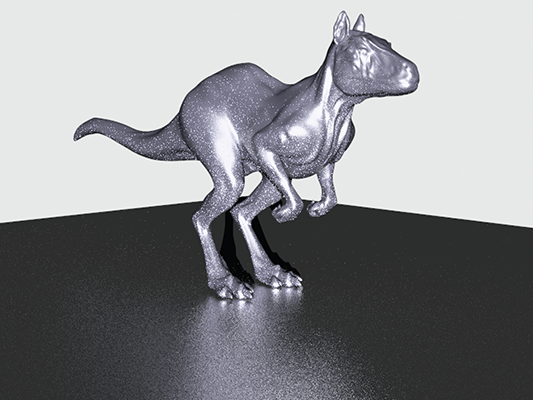
\includegraphics[height=2.2in]{img/IMP_0-2.png}
		\caption{Importance sampling the BRDF}
	\end{subfigure}
	\caption[Importance of Importance Sampling]{A comparison of same time rendering of w/o importance sampling and w/ importance sampling. Notice the obvious difference in the variance level on the ground. (Images courtesy of \citeauthor{PBRT3e})}
	\label{fig:IMP:importance}
\end{figure}
\lettrine{U}{p} until now, we have explored techniques to pre-calculate various terms in the rendering equation (equations \ref{eq:renderEquation:hemisphere}, \ref{eq:renderEquation:threePoint} and \ref{eq:renderEquation:dirIndir}), from irradiance to radiance, from flux to visibility.
These terms all either directly contribute to the final render or indirectly contribute by acting as a guidance for importance sampling.
\figurename \ref{fig:IMP:importance} shows an example of importance sampling the BRDF, which is an analytical term in the rendering equation.
In a sense, if we are using pre-calculated values for importance sampling purposes, we are actually performing importance caching.

\citeauthor{georgiev2012importance} first proposed the technique of \textit{importance caching} in \citeyear{georgiev2012importance} \cite{georgiev2012importance}.
This chapter will build mostly on top of his work.
In this chapter, we discuss techniques to \textit{explicitly cache importance}.
We talk more about importance itself in section \ref{sec:imp_cache:importance} to get a better sense of the importance of \textit{importance}.
In section \ref{sec:imp_cache:algorithm}, we present the algorithm overview of this caching scheme.
We discuss the representations of importance and ways to calculate them in section \ref{sec:imp_cache:represent}, and briefly talk about the accompanied data structure in section \ref{sec:imp_cache:data_structure}.
We finally talk about ways to use this cache in rendering and present applications of similar techniques in different contexts in section \ref{sec:imp_cache:use_cache}.

\section{All About Importance}
\label{sec:imp_cache:importance}
Importance, as we briefly discussed in section \ref{sec:GI:formulation:MC}, is a term to indicate how much a region contributes to the final result.
The more contribution there is, the higher the importance.
From a statistical perspective, importance sampling is about determining certain properties of one distribution using another distribution.
In our case, global illumination, where we are using Monte Carlo integration techniques to solve the equation, we want to sample as proportional to the final contribution as possible.

Most of the time, importance sampling for a 1-D variable in rendering is done by using a random number $\xi$ that is uniformly distributed in range $[0,1]$ to inversely sample a CDF, which is constructed by accumulating a desired PDF.
In discrete cases, corresponding terms are \textit{cumulative mass function}, CMF and \textit{probability mass function}, PMF.

Recall in previous chapters when we use certain terms as importance, we are all dealing with discrete cases.
We build certain PMFs, and consequently CMFs, from finitely many cache records, and normalize the resulting histogram-like information.
In BSDF importance sampling, we sample according to the analytical expression of function, i.e.\ $p \propto f_s$.
In photon driven importance sampling (see section \ref{sec:PM:more:importance}), we pick $p \propto f_s d^2 \Phi / dA$, where $\Phi$ is the information cached in a photon map.
In visibility caching for direct illumination (see section \ref{sec:VC:render:direct}), we pick $p \propto L f_s G \widetilde{V}$, where $\widetilde{V}$ is the information cached in a visibility cache.

It is now clear that we can use any term that appears in the rendering equation as a guidance for importance sampling, analytical or not.
Now we categorize samples using statistical jargon.
We consider those samples that are sampled with decent probability as positive, those with low probability as negative.

\begin{figure}[!ht]
	\begin{subfigure}{0.25\textwidth}
		\centering
		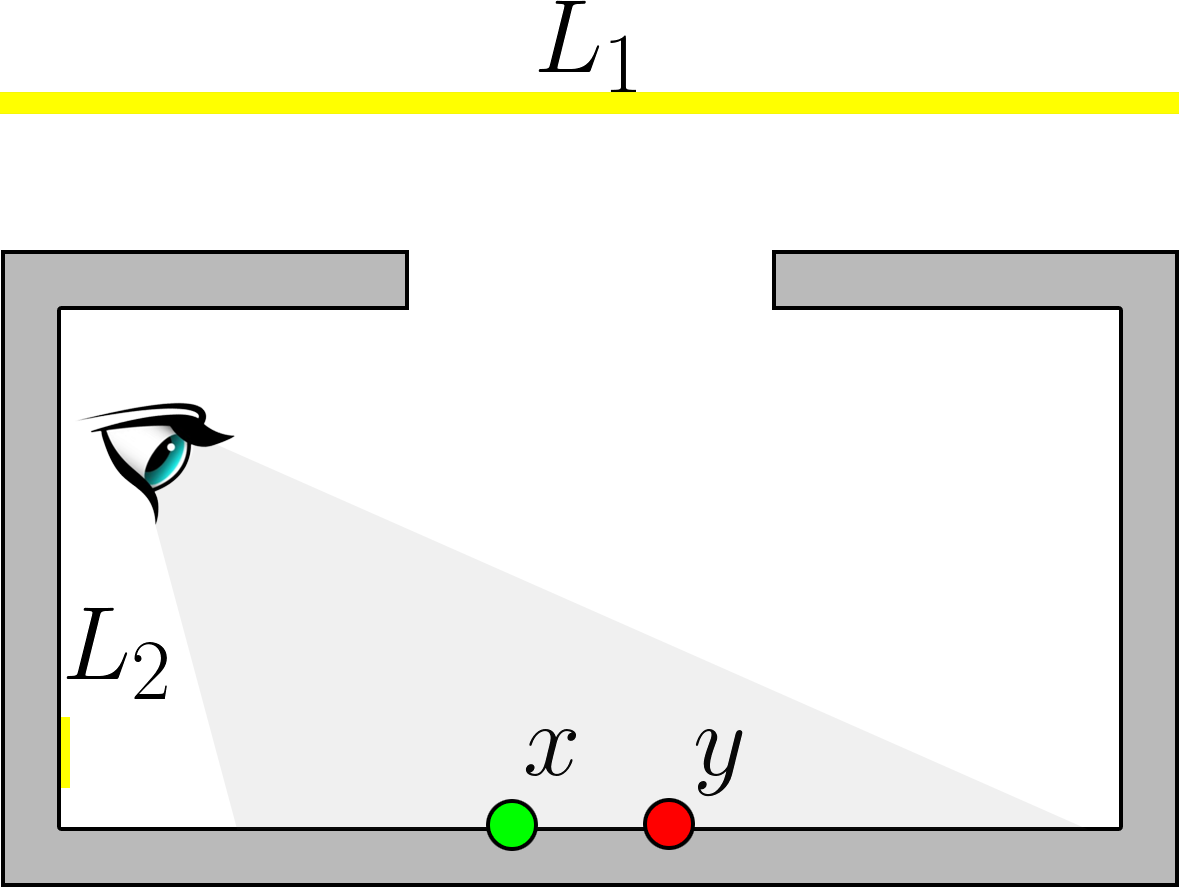
\includegraphics[height=1.1in]{img/IMP_1_1.png}
		\caption{Scene setup}
		\label{fig:IMP:sampleClasses:a}
	\end{subfigure}%
	\begin{subfigure}{0.25\textwidth}
		\centering
		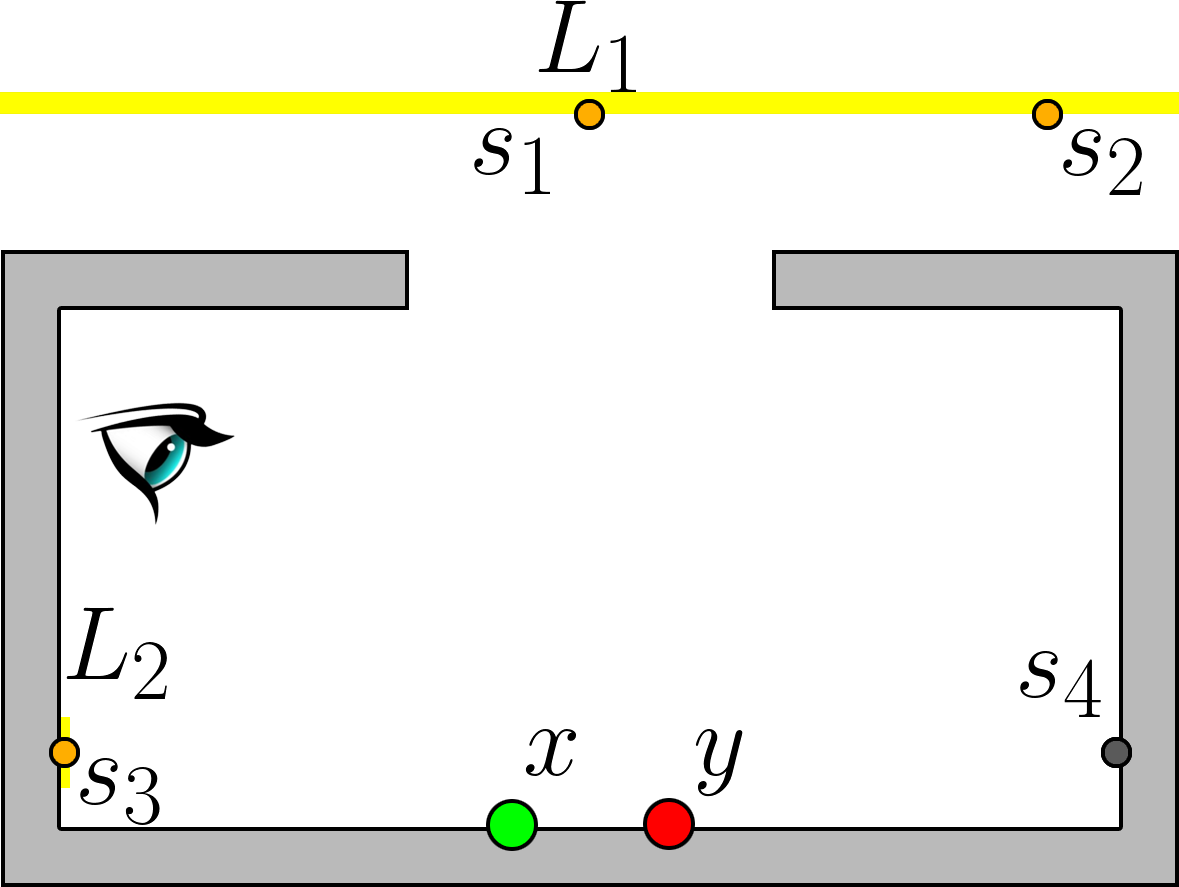
\includegraphics[height=1.1in]{img/IMP_1_2.png}
		\caption{Four samples}
		\label{fig:IMP:sampleClasses:b}
	\end{subfigure}%
	\begin{subfigure}{0.25\textwidth}
		\centering
		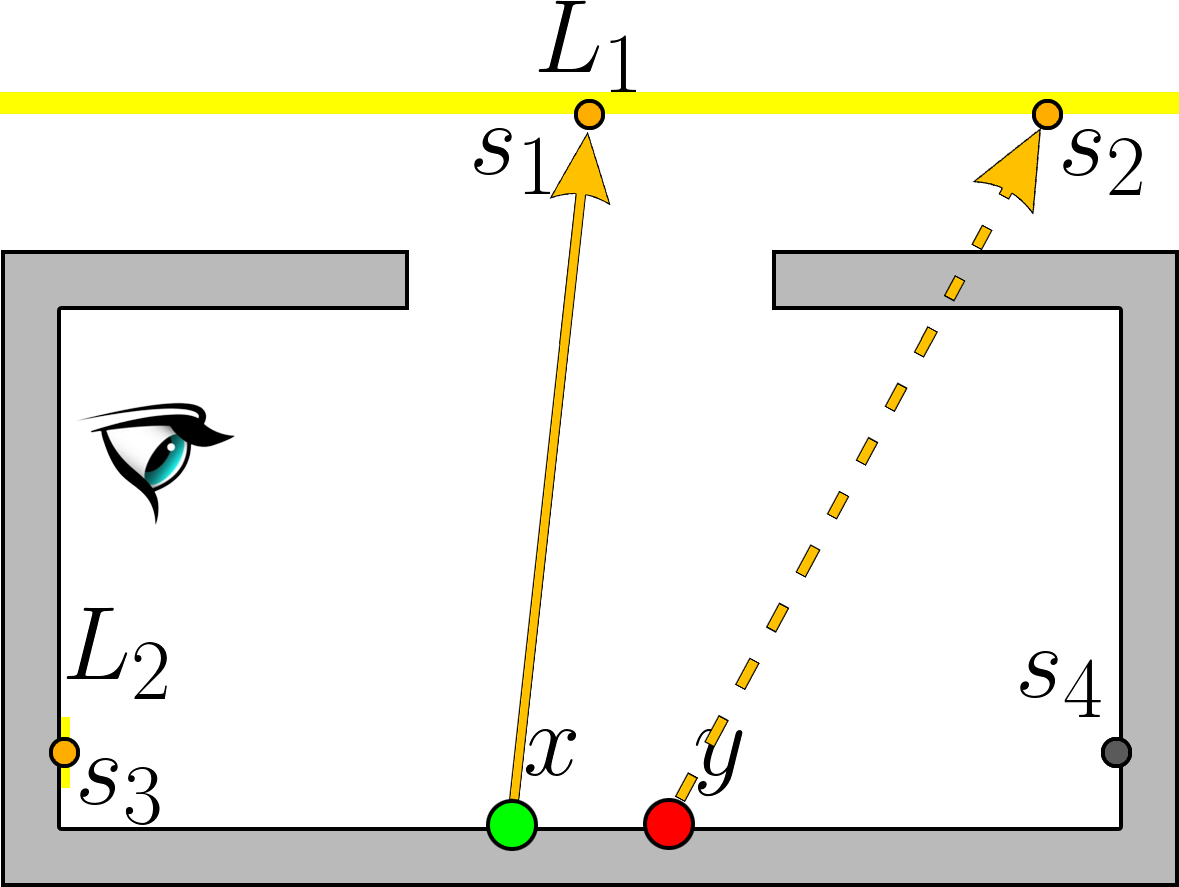
\includegraphics[height=1.1in]{img/IMP_1_3.png}
		\caption{TP and FP}
		\label{fig:IMP:sampleClasses:c}
	\end{subfigure}%
	\begin{subfigure}{0.25\textwidth}
		\centering
		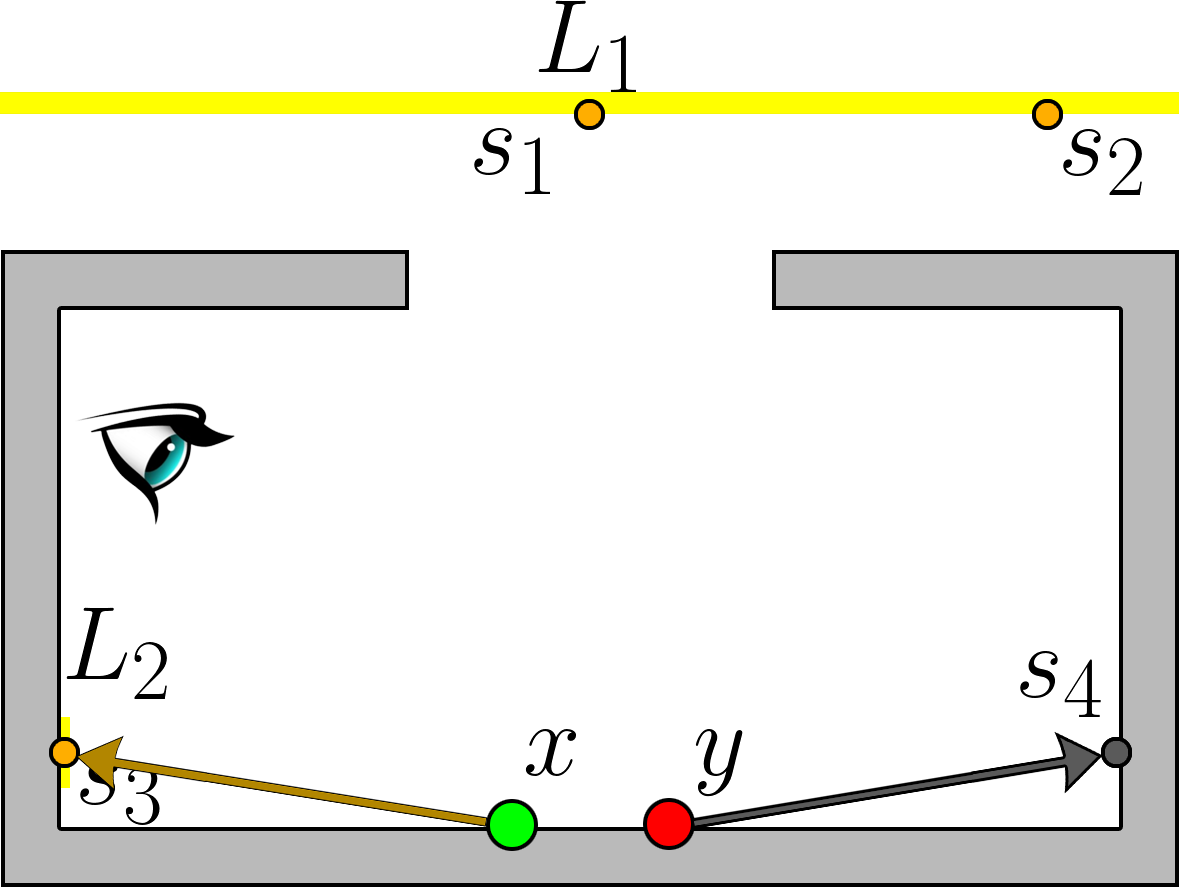
\includegraphics[height=1.1in]{img/IMP_1_4.png}
		\caption{TN and FN}
		\label{fig:IMP:sampleClasses:d}
	\end{subfigure}
	\caption[Classifying Samples]{(a) Two area lights, two shading points. The bigger light $L_1$ lies outside the box, the smaller light $L_2$ lies inside the box but close to ground. Viewpoint is inside the box. Two shading points $x$ and $y$ located in the frustum. (b) Four samples. $s_1$ and $s_2$ lie on $L_1$, $s_1$ is visible to $x$ and $y$ but $s_2$ is occluded to both. $s_3$ lies on $L_2$. $s_4$ lies in the box, close to ground, but not shaded (due to limited depth). (c) Yellow arrow: true positive. Yellow dotted arrow: false positive. (d) Dark yellow arrow: false negative. Grey arrow: true negatives.}
	\label{fig:IMP:sampleClasses}
\end{figure}

\subsubsection*{True Positives}
True positive samples refer to those samples that are sampled with a decent probability according to a PDF and turn out to make decent contribution.
One example is shown in \figurename \ref{fig:IMP:sampleClasses:c}.
Intuitively, TP samples are desirable samples.
\subsubsection*{False Positives}
False positive samples refer to those samples that are sampled with decent probability but turns out to contribute little to the final result.
This kind of sample is usually the source of dark pixels in the noise.
One example is shown in \figurename \ref{fig:IMP:sampleClasses:c}, where $s_2$ is sampled with good probability but is occluded.
\subsubsection*{True Negatives}
True negative samples refer to those samples that are sampled with a low probability and turn out to contribute very little to the final image.
This kind of samples usually would not cause huge amount of variance, since the low contribution will be divided by the low probability. 
One example of such sample is shown in \figurename \ref{fig:IMP:sampleClasses:d}.
TN samples are acceptable samples.
\subsubsection*{False Negatives}
False negatives refer to those samples that are sampled with a low probability but turn out to have decent contribution.
This kind of samples is the main source of the bright spots in the noise, as the decent contribution will be divided by the very low probability and the variance will explode.
One example is shown in \figurename \ref{fig:IMP:sampleClasses:d}, where $s_3$ is sampled with very low probability but turn out to have decent contribution.

As discussed above, the majority of the excessive noise that we can perceive comes from false samples.
False negative samples are particularly undesirable.
To avoid this, we would like an importance sampling technique that could better handle all cases in general.
Next, we present the importance caching algorithm proposed by \citeauthor{georgiev2012importance} to attach this problem.

\section{Algorithm Overview}
\label{sec:imp_cache:algorithm}
The original algorithm by \citeauthor{georgiev2012importance} was designed in the context of \textit{Many-light rendering}, of which \textit{instant radiosity} algorithm by \citeauthor{keller1997VPL} \cite{keller1997VPL} is a major choice.
We first briefly present instant radiosity and many-light rendering in section \ref{sec:imp_cache:algorithm:IR}, and then discuss a importance driven distribution of \textit{virtual point light}s, VPLs, in section \ref{sec:imp_cache:algorithm:distribute}.
In section \ref{sec:imp_cache:algorithm:cacheRender} we briefly overview the rest of the algorithm.

\subsection{Instant Radiosity and Many-light Rendering}
\label{sec:imp_cache:algorithm:IR}
Many-light rendering is a bidirectional global illumination technique that was pioneered by instant radiosity.
The idea is to use finite amount of virtual lights to simulate otherwise infinitely many light samples.
Instant radiosity is a two-pass algorithm, of which a general overview of instant radiosity algorithm goes as follows.

In the first pass, sample certain amount of points on light sources and perform light tracing into the scene.
At each non-specular bounce, create a VPL with its illumination property determined by incoming radiance and surface property.
Certain amount of VPLs are created on light sources as well.
Stop light tracing at certain depth.
In the second pass, trace rays from the camera into the scene.
At first non-specular hits, connecting shading points with all VPLs.
The resulting radiance is the sum of contributions from all $N$ VPLs, and the formulation is given as
\begin{equation}
	\widehat{I}_{ml}(\textbf{x}_i) = \sum_{k=1}^{N}L(\textbf{x}_i \leftarrow \textbf{v}_k) f_s(\textbf{x}_{i-1} \leftarrow \textbf{x}_i \leftarrow \textbf{v}_k) G(\textbf{x}_i \leftarrow \textbf{v}_k) V(\textbf{x}_i \leftrightarrow \textbf{v}_k)
	\label{eq:IMP:ML}
\end{equation}

The nature of using finite amount of direct illumination to approximate global illumination makes many-light rendering a viable choice for many interactive applications.
Few of the advantages thereof include scalability and easy implementation on graphics hardwares using rasterization.
However, many-light rendering does have its limitation.
The most obvious limitation is that it is a biased technique.
Another exemplary disadvantage is the strong correlated sampling as a consequence of reusing a same set of VPLs.
Please refer to the \textit{STAR} report on the same topic by \citeauthor{dachsbacher2014scalable} for more details about instant radiosity and many-light rendering \cite{dachsbacher2014scalable}.

For the purpose of a better algorithm overview, the pseudo code for importance caching is now given in \textcolor{blue}{Algorithm} \ref{alg:IMP:impCache}.
Detailed pseudo code is given in respective sections later.

\begin{algorithm}[b]
	\caption[Importance Caching]{Pseudo code for Importance Caching}
	\addtocontents{loa}{\vskip 4pt}
	\label{alg:IMP:impCache}
	\begin{algorithmic}[1]
		\Procedure{ImportanceCaching}{\textbf{scene}}
			\State \textbf{V} $\gets$ \textsc{DistributeVPL}(\textbf{scene})
			\State \textbf{IC} $\gets$ \textsc{BuildImpCache}(\textbf{scene}, \textbf{V})
			\State \textsc{FinalRender}(\textbf{scene}, \textbf{V}, \textbf{IC})
		\EndProcedure
	\end{algorithmic}
\end{algorithm}

\subsection{Importance-driven VPL Distribution}
\label{sec:imp_cache:algorithm:distribute}
In standard instant radiosity, VPLs are distributed using light tracing.
For a fixed amount of records, this will result in evenly distributed VPLs according to true illumination distribution.
However, this might not be optimal.
For scenes with difficult visibility, the majority of VPLs will probably lie outside the visible region seen from the camera.

Importance-driven VPL distribution was proposed by \citeauthor{georgiev2010simple} as an extension to standard VPL distribution process \cite{georgiev2010simple}.
The extension is to first run few pilot VPL distributions and render a low resolution image to get an estimate of average VPL contribution $\Phi_v$.
Next, during the light tracing pass of VPL distribution, rather than simply accept a bounce $v_i$ as a VPL, a Russian roulette is used to determine whether current record $v_i$ is accepted or not.
The acceptance probability $p_i$ is determined by $p_i = \textup{min}\left\{ \frac{\Phi_i}{\Phi_v} + \epsilon, 1 \right\}$, where $\Phi_i$ is the contribution of current candidate to $v_i$ the image plane as one big pixel and $\epsilon$ is a tiny value to avoid zero probability.
If records are rejected, current random walk of light tracing will simply be terminated.
Otherwise, flux carried by the accepted records will be divided by $p_i$ as what other techniques do when using Russian roulette to ensure unbiasedness.

The process is summarized in \textcolor{blue}{Algorithm} \ref{alg:IMP:DistribVPL} and \figurename \ref{fig:IMP:buildCacheRender:a}.

\begin{algorithm}[t]
	\caption[VPL Distribution]{Pseudo code for VPL distribution}
	\addtocontents{loa}{\vskip 4pt}
	\label{alg:IMP:DistribVPL}
	\begin{algorithmic}[1]
		\Procedure{DistributeVPL}{\textbf{scene}}
			\State $V \gets \emptyset$
			\State $V_p \gets$ Run a few pilot VPL distributions
			\State $\Phi_v \gets$ Average contribution for each VPL in $V_p$
			\State \textit{Start light tracing, for each sample:}
			\While{Random walk not terminated}
				\If{Hit non specular surface}
					\State $\Phi_i \gets$ Calculate contribution of current $v_i$
					\State $p_i = \textup{min}\left\{ \frac{\Phi_i}{\Phi_v} + \epsilon, 1 \right\}$
					\If{\textsc{RussianRoulette}($p_i$)}
						\State $v_i$.flux $\mathrel{{\div}{=}} p_i$
						\State $V \xleftarrow{insert}$ Create a VPL using updated $v_i$
						\State Continue random walk
					\Else
						\State Terminate random walk
					\EndIf
				\Else
					\State Continue random walk
				\EndIf
			\EndWhile
			\State \Return $V$
		\EndProcedure
	\end{algorithmic}
\end{algorithm}

\subsection{Caching Importance and Final Rendering}
\label{sec:imp_cache:algorithm:cacheRender}
The idea of importance caching in the context of many-light rendering is to evaluate exact contribution at a sparse set of points in scene and cache them in a first pass.
In the second pass, at each shading point, the importance distribution of current point is approximated by interpolating valid importance cache records nearby.
When the approximated importance distribution is available, we can importance sample this distribution and continue with regular Monte Carlo rendering.
This whole process is illustrated in \figurename \ref{fig:IMP:buildCacheRender}.
Next, we discuss the exact representations for importance, reasoning behind them and ways to calculate them.
\begin{figure}[!ht]
	\begin{subfigure}{0.25\textwidth}
		\centering
		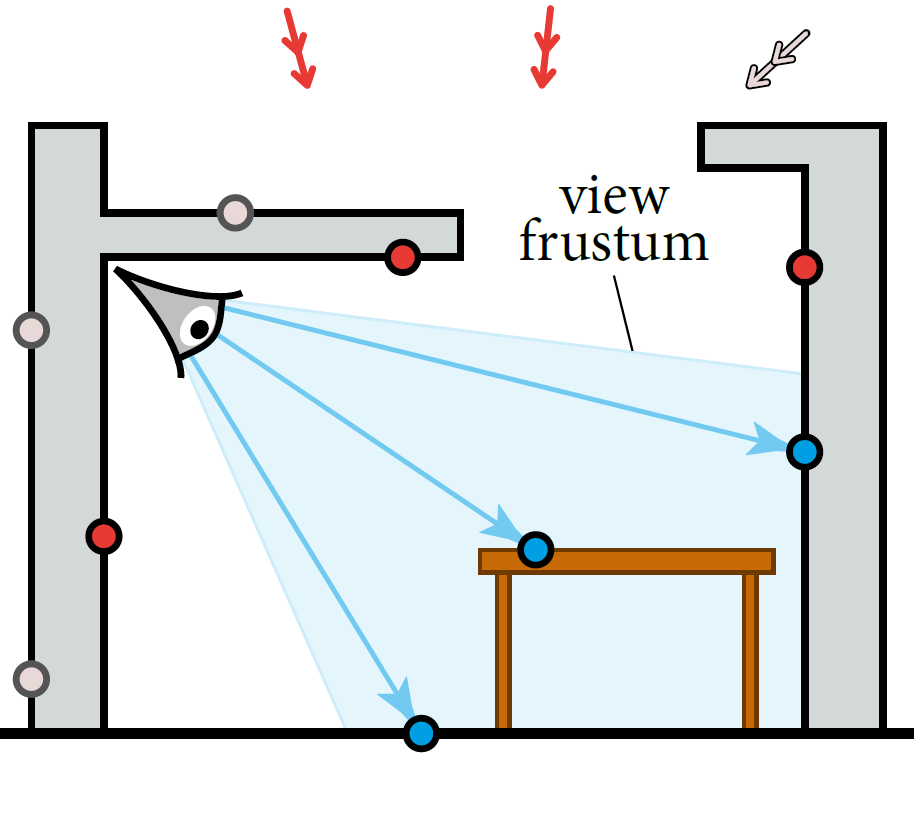
\includegraphics[height=1.3in]{img/IMP_2_1.png}
		\caption{}
		\label{fig:IMP:buildCacheRender:a}
	\end{subfigure}%
	\begin{subfigure}{0.25\textwidth}
		\centering
		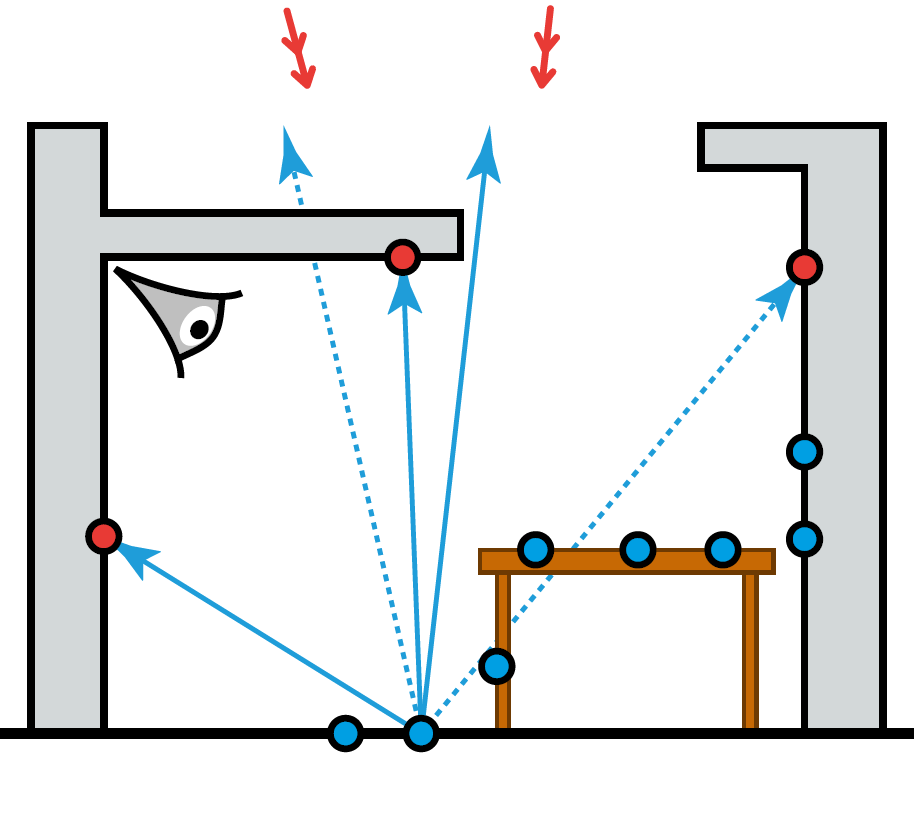
\includegraphics[height=1.3in]{img/IMP_2_2.png}
		\caption{}
	\end{subfigure}%
	\begin{subfigure}{0.25\textwidth}
		\centering
		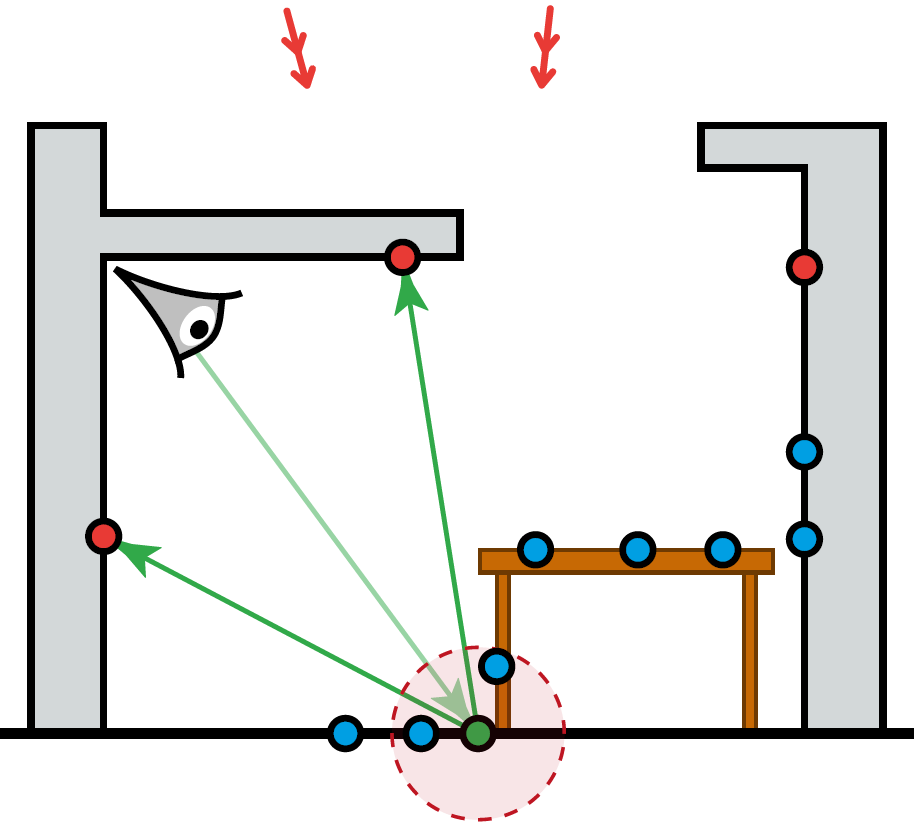
\includegraphics[height=1.3in]{img/IMP_2_3.png}
		\caption{}
	\end{subfigure}%
	\begin{subfigure}{0.25\textwidth}
		\centering
		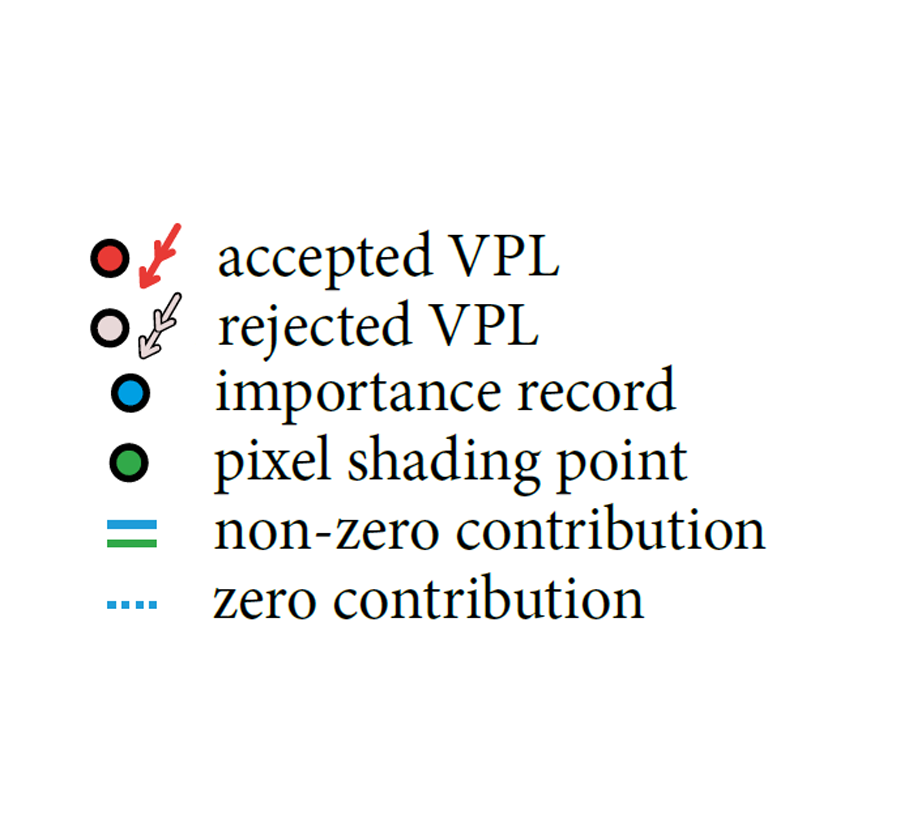
\includegraphics[height=1.3in]{img/IMP_2_4.png}
		%\caption{}
	\end{subfigure}
	\caption[Building and Using Importance Cache]{(a) Importance-driven VPL distribution. Red dots are accepted VPLs. (b) Evaluate contributions from all VPLs at each sample of a sparse set of points, blue points. Create importance records at these points. (c) Rendering with importance cache. At each shading point, green point, locate usable importance cache records, blue points within the circle. Importance sample according to the interpolation of these cache records. (Images courtesy of \citeauthor{georgiev2012importance})}
	\label{fig:IMP:buildCacheRender}
\end{figure}

\section{Importance Representation}
\label{sec:imp_cache:represent}
From what we discussed above, we can see that an importance cache is a normalized histogram, with each bin representing the contribution ratio of a respective VPL.
Intuitively, this contribution is the true and full contribution of each VPL, i.e.\ $L_i f_s G_i V_i$.
However, due to the interpolation nature, which assumes smooth variation and strong correlation, this scheme might fail to work well at discontinuities.
To robustly handle these difficult cases, which are common, it might be helpful to think differently.
Recall in section \ref{sec:imp_cache:importance}, we want TP and TN, FP is ok, but FN is hardly desirable.
As we will shortly find out, a combination of the four terms in $L_i f_s G_i V_i$ makes result more robust.

\begin{figure}[t]
	\begin{subfigure}{0.25\textwidth}
		\centering
		\includegraphics[height=1.4in]{img/IMP_3_1.png}
		\caption{}
		\label{fig:IMP:represent:a}
	\end{subfigure}%
	\begin{subfigure}{0.25\textwidth}
		\centering
		\includegraphics[height=1.4in]{img/IMP_3_2.png}
		\caption{}
		\label{fig:IMP:represent:b}
	\end{subfigure}%
	\begin{subfigure}{0.25\textwidth}
		\centering
		\includegraphics[height=1.4in]{img/IMP_3_3.png}
		\caption{}
		\label{fig:IMP:represent:c}
	\end{subfigure}%
	\begin{subfigure}{0.25\textwidth}
		\centering
		\includegraphics[height=1.4in]{img/IMP_3_4.png}
		\caption{}
		\label{fig:IMP:represent:d}
	\end{subfigure}
	\caption[Four Distributions]{Four cases for importance distribution. (a) Full distribution. (b) Un-occluded distribution. (c) Bounded distribution. (d) Conservative distribution. (Images courtesy of \citeauthor{georgiev2012importance})}
	\label{fig:IMP:represent}
\end{figure}

\subsection{$\boldsymbol{F}$: Full Distribution}
\label{sec:imp_cache_represent:F}
Full distribution is, by its name, the full contribution of each VPL, i.e.\ for each VPL, we compute $\boldsymbol{F} \mathrel{{:}{=}} L f_s G V$.
This distribution performs best in cases where surfaces vary smoothly and the occlusion situation remains pretty much the same.
See \figurename \ref{fig:IMP:represent:a}, where two importance cache records $\mathbf{r}_1$ and $\mathbf{r}_2$ capture the true illumination at $\mathbf{x}$.

\subsection{$\boldsymbol{U}$: Un-occluded Distribution}
\label{sec:imp_cache_represent:U}
Discontinuities, as mentioned earlier, happen quite often.
The main source of discontinuities is occlusion changes.
See the case in \figurename \ref{fig:IMP:represent:b}, where both $\mathbf{r}_1$ and $\mathbf{r}_2$ see $\mathbf{v}_1$ but not $\mathbf{v}_2$, which is the other way around for $\mathbf{x}$.
In this case, if we sample according to full distribution, we will get a false positive, which is less desirable.
Thus it would be helpful to take occlusion out of consideration, to some extent.
The un-occluded distribution is the contribution of each VPL without considering the visibility term, i.e.\ $\boldsymbol{U} \mathrel{{:}{=}} L f_s G$.

\subsection{$\boldsymbol{B}$: Bounded Distribution}
\label{sec:imp_cache_represent:B}
Sometimes for a shading point, nearby cache records will give low probabilities to some VPLs that are actually making a decent amount of contribution.
This is the case of false negatives, which we want the least.
One of such cases is caused by the geometry term, for which $G_{\mathbf{r}} < G_{\mathbf{x}}$, where $\mathbf{r}$ is cache record and $\mathbf{x}$ is a shading point.
See the example in \figurename \ref{fig:IMP:represent:b}, for which case if we sample $\mathbf{v}_1$ according to the distributions gathered from $\mathbf{r}_1$ and $\mathbf{r}_2$, resulting value will explode due to the very small probability.

False negatives caused by geometry term is handled by $\boldsymbol{B}$, the bounded distribution, which act as an extension to $\boldsymbol{U}$.
For each record $\mathbf{r}_j$, we assign a valid region of influence with a radius $r_j$.
Within the region, there are variations in position and normal orientation.
Among all the range, we calculate the maximum value for the geometry term, $G_j$.
Recall in equation \ref{eq:renderEquation:threePoint}, $G = V \frac{|\cos\theta \cos\phi|}{d^2}$.
We take out the visibility term $V$ as we did for $\boldsymbol{U}$, and the maximum geometry term is defined as
\begin{equation*}
	G^{max} (\mathbf{r}_j, \mathbf{v}_k)= \frac{|\cos\theta_j^{min} \cos\theta_k^{min}|}{(d^{min})^2}
\end{equation*}
where term $\theta_j^{min}$, $\theta_k^{min}$ and $d^{min}$ is defined in \figurename \ref{fig:IMP:represent:bound}.
For virtual lights with a surface point form, see \figurename \ref{fig:IMP:represent:bound:b}.
For virtual lights with a directional light form, see \figurename \ref{fig:IMP:represent:bound:a}, where the gray arrow indicate the surface normal within influence region that has the smallest angle with the virtual light.

\begin{figure}[t]
	\begin{subfigure}{0.5\textwidth}
		\centering
		\includegraphics[height=1.6in]{img/IMP_3B_1.png}
		\caption{}
		\label{fig:IMP:represent:bound:a}
	\end{subfigure}%
	\begin{subfigure}{0.5\textwidth}
		\centering
		\includegraphics[height=1.6in]{img/IMP_3B_2.png}
		\caption{}
		\label{fig:IMP:represent:bound:b}
	\end{subfigure}
	\caption[Bounded Distribution]{Bounded distribution between cache record $\mathbf{r}_j$ and VPL $\mathbf{v}_k$. (a) For case when the virtual light is a virtual directional/ray light. The gray line indicate the surface with the smallest normal angle within the influence region of cache record $\mathbf{r}_j$. (b) For case when the virtual light is a point light on surface. (Images courtesy of \citeauthor{georgiev2012importance})}
	\label{fig:IMP:represent:bound}
\end{figure}

The bounded distribution is then defined as $\boldsymbol{B} \mathrel{{:}{=}} L f_s G^{max}$.
Now, for cases like \figurename \ref{fig:IMP:represent:b}, for cache record $\mathbf{r}_2$, VPL $\mathbf{v}_1$ will be assigned a decent share of importance.
Consequently $\mathbf{v}_1$ will be sampled with a decent probability at $\mathbf{x}$, thus avoiding the explosive noise.
In practice, $\boldsymbol{B}$ can help find VPLs with small contributions.

\subsection{$\boldsymbol{C}$: Conservative Distribution}
\label{sec:imp_cache_represent:C}
For the worst case scenario, no records can provide useful information to a shading point.
Such a case is shown in \figurename \ref{fig:IMP:represent:d}, where non of the cache records are relevant for $\mathbf{x}$, much like the case in \figurename \ref{fig:IMP:represent:b}.
However, if sampled in the way as in un-occluded distribution, $\mathbf{v}_2$ and $\mathbf{v}_3$ are still very likely to be sampled while the only true option is $\mathbf{v}_1$.

For such cases with complex visibility, it is worth the expense to add another distribution that is uniform for all VPLs.
The conservative distribution, $\boldsymbol{C}$, is thus defined as $\boldsymbol{C} \mathrel{{:}{=}} \frac{1}{\textup{card}(VPLs)}$.

Now, the process of representing and calculating caches is clear.
The whole process is summarized in \textcolor{blue}{Algorithm} \ref{alg:IMP:buildCache}, where line 2 is pretty much identical to methods in previous chapters when we distribute points through out the scene.

\begin{algorithm}[b]
\caption[Build Importance Cache]{Pseudo code for building Importance Cache}
\addtocontents{loa}{\vskip 12pt}
\label{alg:IMP:buildCache}
\begin{algorithmic}[1]
	\Procedure{BuildImpCache}{\textbf{scene}, \textbf{V}}
		\State $\boldsymbol{R} \gets$ distribute cache candidates on non-specular surfaces in \textbf{scene}
		\ForAll{cache candidate \textbf{r} in $\boldsymbol{R}$}
			\State $f_s \gets$ surface BSDF at \textbf{r}
			\ForAll{VPL \textbf{v} in \textbf{V}}
				\State $L\gets$ radiance contribution from \textbf{v} to \textbf{r}
				\State $G\gets \frac{|\cos\theta_{\textbf{r}} \cos\theta_{\textbf{v}}|}{d^2}$
				\State $G^{max}\gets\frac{|\cos\theta_{\textbf{r}}^{min} \cos\theta_{\textbf{v}}^{min}|}{(d^{min})^2}$
				\State $V\gets$ shadow ray visibility test between \textbf{v} and \textbf{r}
				\State $\mathbf{r}$.$\boldsymbol{F} \gets L f_s G V$
				\State $\mathbf{r}$.$\boldsymbol{U} \gets L f_s G$
				\State $\mathbf{r}$.$\boldsymbol{B} \gets L f_s G^{max}$
				\State $\mathbf{r}$.$\boldsymbol{C} \gets \frac{1}{\textup{card}(V)}$
			\EndFor
		\EndFor
		\State \Return $\boldsymbol{R}$
	\EndProcedure
\end{algorithmic}
\end{algorithm}

\section{Data Structure}
\label{sec:imp_cache:data_structure}
Since the importance caching algorithm is actually a three-pass algorithm, two structures will be needed to hold data from the first two passes.
For the first pass, where VPLs are distributed according to visual importance, the end result for later use is to answer indexed queries.
For this reason, data structure for VPLs does not need to handle tasks such as range queries or nearest neighbors.
Thus, an indexed array suffices to be the data structure for VPLs.

For the second pass, where importance cache records are created and stored, the end result will need to answer range queries and nearest neighbor searches.
Given the experience we had from previous chapters, a \textit{k}-d tree is a perfect choice.

\section{Using the Importance Cache}
\label{sec:imp_cache:use_cache}
The core idea of using importance sampling for many-light rendering is that sometime there might be too many virtual lights, explicitly evaluating them one by one is prohibitively expensive.
Thus using our cached importance as a guidance, we importance sample a smaller set of whole VPLs.
The estimator from equation \ref{eq:IMP:ML} for this process is given as
\begin{equation}
	\widehat{I}_{ml} \approx \sum_{k=1}^{M} \frac{L(\textbf{x}_i \leftarrow \textbf{v}_k) f_s(\textbf{x}_{i-1} \leftarrow \textbf{x}_i \leftarrow \textbf{v}_k) G(\textbf{x}_i \leftarrow \textbf{v}_k) V(\textbf{x}_i \leftrightarrow \textbf{v}_k)}{p(\textbf{v}_k|\textbf{x}_i)} = \widehat{I}_{ic}
	\label{eq:IMP:IC}
\end{equation}
where $M<N$, representing the number of Monte Carlo samples used to approximate the full set of VPLs.

Before we can make proper use of existing caches, we need to locate them in the query structure.
A similar weighting function as equation \ref{eq:IC:weight} is used, and the metric is defined as
\begin{equation}
	d(\textbf{x}, \textbf{r}_j) =  \left \| \textbf{x} - \textbf{r}_j \right \| + \lambda \sqrt{1 - n_{\textbf{x}} \cdot n_{\textbf{r}_j}}.
\end{equation}
where $\lambda$ is a user specified value to balance preference for distance or normal difference.

So far in each cache record, there are four distributions, with each one being a normalized histogram comprising $N_{VPL}$ bins.
One way to use these information is to interpolate.
We can assign each record a weight according to their spatial distance and normal difference.
However, this style of combination works on one dimensional values, in our case we are facing with an importance distribution matrix, see \figurename \ref{fig:IMP:records}.

\citeauthor{georgiev2012importance} proposed a \textit{bilateral combination} technique to take advantage of the strengths of each record \cite{georgiev2012importance}.
We next briefly present the method.
At last, we discuss the application of similar spirit in the context of PT \cite{bashford2012significance} and BDPT \cite{popov2015probabilistic}.

\begin{figure}[b]
	\centering
	\includegraphics[height=1.4in]{img/IMP_5a.png}
	\caption[Importance Distribution Matrix]{Three importance cache records located near a shading point, with four distributions in a matrix layout. The goal of combining these distributions is to preserve their ability to handle unique cases as mentioned in the previous section. (Images courtesy of \citeauthor{georgiev2012importance})}
	\label{fig:IMP:records}
\end{figure}

\subsection{Bilateral Combination of Cache Distributions}
\label{sec:imp_cache:use_cache:combine}
The bilateral combination is a two step operation on the distribution matrix.
In the first step, an MIS estimator is used to combine cache records in rows.
The rest four distributions in the combined one column distribution is then combined using another heuristic for final use.
\subsubsection*{Column Combination}
For all four rows, viz.\ $1: \boldsymbol{F}$, $2: \boldsymbol{U}$, $3: \boldsymbol{B}$ and $4: \boldsymbol{C}$, the MIS estimator for row $i \in \{1, 2, 3, 4\} $ is given as
\begin{equation}
	\widehat{I}_{mis} (\textbf{x}_o, \textbf{x}, i) = \sum_{j=1}^{M} \frac{1}{n_i}\sum_{k=1}^{n_i}w_{i,j}^{col}(\textbf{x}_o, \textbf{x}, v_{i,j,k})\frac{L(\textbf{x}\leftarrow v_{i,j,k}) f_s(\textbf{x}_o \leftarrow \textbf{x}\leftarrow v_{i,j,k}) G(\textbf{x}\leftarrow v_{i,j,k}) V(\textbf{x}\leftrightarrow v_{i,j,k})}{p(v_{i,j,k}|\textbf{x})}
	\label{eq:IMP:column01}
\end{equation}
where $M$ is the number of cache records, $n_i$ is number of samples that remains constant across rows, $\textbf{x}$ is current scattering point and $\textbf{x}_o$ is the out going point, i.e.\ viewed from $\textbf{x}_o$.

The weight function uses the balanced heuristic from \cite{veach1995MIS}, which is given in the form of 
\begin{equation*}
	w_{i,j}^{col}(\textbf{x}_o, \textbf{x}, v_{i,j,k}) = \frac{p_{i,j}(\textbf{x}_o, \textbf{x}, v_{i,j,k})}{\sum_{l=1}^{M}p_{i,l}(\textbf{x}_o, \textbf{x}, v_{i,l,k})},
\end{equation*}
thus equation \ref{eq:IMP:column01} can be reduced to
\begin{equation}
	\widehat{I}_{mis} (\textbf{x}_o, \textbf{x}, i) = \frac{1}{n_i} \sum_{k=1}^{n_i} \frac{L(\textbf{x}\leftarrow v_{i,k}) f_s(\textbf{x}_o \leftarrow \textbf{x}\leftarrow v_{i,k}) G(\textbf{x}\leftarrow v_{i,k}) V(\textbf{x}\leftrightarrow v_{i,k})}{p(v_{i,k}|\textbf{x})}.
\label{eq:IMP:column02}
\end{equation}

\subsubsection*{Row Combination}
Now we have for each row an estimated value, viz.\ $\widehat{I}_{mis} (\textbf{x}_o, \textbf{x}, \boldsymbol{F})$, $\widehat{I}_{mis} (\textbf{x}_o, \textbf{x}, \boldsymbol{U})$, $\widehat{I}_{mis} (\textbf{x}_o, \textbf{x}, \boldsymbol{B})$ and $\widehat{I}_{mis} (\textbf{x}_o, \textbf{x}, \boldsymbol{C})$.
All we need to do is to combine these four values into one.

Weighted combination of four values can easily break the advantages each distribution has for handling specific situations.
See \figurename \ref{fig:IMP:combination:a}, where a combination using balanced heuristic $p_b$ results in significant amount of variance.
Thus it is better to take a step further and divide the whole domain and pick one suitable distribution for a specific situation instead of weighting all four distribution in the same way through out the domain.

\subsubsection*{$\alpha$-max Heuristic}
\citeauthor{georgiev2012importance} proposed a $\alpha$-max heuristic to solve this problem.
The $\alpha$-max heuristic is expressed as
\begin{equation}
	w_s^\alpha(x) = \begin{cases}
	1, & \text{ if } w_i^\alpha(x) = 0, \textup{for } 1 \leq i < s, \textup{ and } p_s(x)\geq \underset{s<i\leq m}{max} \alpha_i p_i(x)\\ 
	0, & \text{ otherwise, } 
	\end{cases}
\end{equation}
where $x$ is sampled according to $p_s$ and $\alpha_i\in (0,1]$ is a confidence value associated with current distribution.

The $\alpha$-max heuristic assigns probability according to which distribution has the highest value, thus reduce variance.
Intuitively, this will partition the domain into several sub-domains, with each one dominated by one distribution.
See \figurename \ref{fig:IMP:combination:b}.

Few results of using importance caching from the original paper \cite{georgiev2012importance} are shown in \figurename \ref{fig:IMP:results}.

\begin{figure}[t]
	\begin{subfigure}{0.5\textwidth}
		\centering
		\includegraphics[height=1.2in]{img/IMP_5b_1.png}
		\caption{}
		\label{fig:IMP:combination:a}
	\end{subfigure}%
	\begin{subfigure}{0.5\textwidth}
		\centering
		\includegraphics[height=1.2in]{img/IMP_5b_2.png}
		\caption{}
		\label{fig:IMP:combination:b}
	\end{subfigure}
	\caption[Bilaterial Combination of Distributions]{(a) $p_b$ is the result of balance heuristic, note the level of variance due to the averaging operation. A uniform distribution $p_u$ ruins all the effort. (b) The $\alpha$-max heuristic. The domain is partitioned into three parts, with each part only using the distribution with the max probability. Notice the variance reduction. (Images courtesy of \citeauthor{georgiev2012importance})}
	\label{fig:IMP:combination}
\end{figure}

\begin{figure}
	\centering
	\includegraphics[width=\textwidth]{img/IMP_5c.png}
	\caption[Importance Caching Results]{Some results rendered using importance caching. The image is rendered using $35$ VPLs per pixel. Different columns represent different strategies. Notice how the strength of each strategy is demonstrated in specific situations. The reference image is rendered using $\boldsymbol{FUBC}^\alpha$ in $1000$ seconds, the rest images all use $20$ seconds. (Images courtesy of \citeauthor{georgiev2012importance})}
	\label{fig:IMP:results}
\end{figure}

\subsection{Similar Applications in PT and BDPT}
\label{sec:imp_cache:use_cache:bdpt}
\citeauthor{bashford2012significance} proposed to store the information of sampling BRDF and cosine term as \textit{significance cache}, and use this significance cache to guide later scattering event \cite{bashford2012significance}.
The cache is represented as reflection lobe.
Results show improved performance at difficult visibility scenarios and reduced variance comparing to regular sampling methods.
While this method could also be categorized as \textit{path guiding}, of which one popular way is to use photon map as a driver, this way of guiding paths shares the same spirit as importance sampling using importance cache.

\citeauthor{popov2015probabilistic} proposed to use importance caching for the vertex connections in BDPT \cite{popov2015probabilistic}.
The method first trace light paths and eye paths into the scene.
Then pick a uniformly distributed set of eye path and evaluate importance at each eye vertex of all pre-generated light paths and create a cache record with corresponding values stored in a normalized PMF.
During rendering, eye paths are generated as usual.
When performing eye-light sub-path connections, at each eye vertex, nearby cache records are located and a combined PMF is calculated via interpolation.
A importance sampled light path is picked by sampling according to this interpolated PMF.
Results show significant improvement on variance reduction and speed up comparing to standard BDPT.

While various methods exist to make smarter choices when picking samples, what they have in common is to match probability with contribution.
Caching, as a reliable technique, provides a glimpse of what the target might look like.
Even though directly using caches results in correlation, using them as a hint guarantees unbiasedness.
We cannot emphasize the importance of importance sampling, as it will always be the goal for Monte Carlo based rendering.

%%%%%%%%%%%%%%%%%%%%%%%%%%%%%%%%%%%%%%%%%%%%%%%%%%%%%%%%%%%%%%%%%%%%%%%%%%%%%%%%%%%%%%%%%%%%%%%%%%%%%%%%%%%%%%%%%%%%%%%%%%%%%%%%%%%%%%%%%%%%%%%%%%%%%%%%%%%%

\chapter{Conclusion}
\label{chap:conclusion}
\lettrine{I}{n} this survey, we studied various caching schemes in the field of global illumination.
We studied irradiance caching and radiance caching, as they are the pioneering caching technique in this field.
We studied photon mapping, of which the original algorithm essentially uses a caching scheme.
We studied visibility caching, which tries to solve issues related to visibility tests.
Finally we explored caching techniques that explicitly targeting at importance.

In each part, we present the problem, the formulation and theoretical foundations of using caches.
We studied representation for the data to cache as well as data structures to hold these cache records.
We studied different ways to make use of cached data.

It is very difficult to make a definite conclusion for caching techniques or for global illumination.
Here we quote \citeauthor{AdvancedGI} from the book \citetitle{AdvancedGI} to conclude this survey, \textit{the quest for realism and speed has not yet come
to an end} \cite{AdvancedGI}.

%%%%%%%%%%%%%%%%%%%%%%%%%%%%%%%%%%%%%%%%%%%%%%%%%%%%%%%%%%%%%%%%%%%%%%%%%%%%%%%%%%%%%%%%%%%%%%%%%%%%%%%%%%%%%%%%%%%%%%%%%%%%%%%%%%%%%%%%%%%%%%%%%%%%%%%%%%%%
% End of content
\printbibliography
\addcontentsline{toc}{chapter}{Bibliography}

\end{document}